

% ----------------------------------------------------------------------
%                   LATEX TEMPLATE FOR PhD THESIS
% ----------------------------------------------------------------------

% based on Harish Bhanderi's PhD/MPhil template, then Uni Cambridge
% http://www-h.eng.cam.ac.uk/help/tpl/textprocessing/ThesisStyle/
% corrected and extended in 2007 by Jakob Suckale, then MPI-CBG PhD programme
% and made available through OpenWetWare.org - the free biology wiki


%: Style file for Latex
% Most style definitions are in the external file PhDthesisPSnPDF.
% In this template package, it can be found in ./Latex/Classes/
\documentclass[twoside, 12pt]{thesis}


%: Macro file for Latex
% Macros help you summarise frequently repeated Latex commands.
% Here, they are placed in an external file /Latex/Macros/MacroFile1.tex
% An macro that you may use frequently is the figuremacro (see introduction.tex)
\newcommand{\comment}[1]{}
\newcommand{\myparagraph}[1]{\paragraph{#1}\mbox{}\\}
\newcommand{\pw}[4]{
	\begin{cases}\displaystyle
		#1 & \mbox{#2},\\ 
		#3 & \mbox{#4}
	\end{cases}
}

\newcommand{\cref}[1]{Chap.~\ref{#1}}
\newcommand{\Cref}[1]{Chapter~\ref{#1}}
\newcommand{\sref}[1]{Sec.~\ref{#1}}
\newcommand{\Sref}[1]{Section~\ref{#1}}
\newcommand{\aref}[1]{App.~\ref{#1}}
\newcommand{\Aref}[1]{Appendix~\ref{#1}}
\newcommand{\fref}[1]{Fig.~\ref{#1}}
\newcommand{\Fref}[1]{Figure~\ref{#1}}
\newcommand{\tref}[1]{Tab.~\ref{#1}}
\newcommand{\Tref}[1]{Table~\ref{#1}}
\newcommand{\pgref}[1]{p.~\pageref{#1}}
\newcommand{\Pgref}[1]{page~\pageref{#1}}



\def\eqrefs#1#2{(\protect\ref{#1}--\protect\ref{#2})}

\newcommand{\alert}[1]{\textcolor{red}{#1}}
\newcommand{\PN}[1][N]{\ensuremath{\text{P}_{#1}}}
\newcommand{\MCPN}[1][N]{\ensuremath{\text{MCP}_{#1}}}
\newcommand{\SN}[1][N]{\ensuremath{\text{S}_{#1}}}
\newcommand{\SPN}[1][N]{\ensuremath{\text{SP}_{#1}}}
\newcommand{\Oh}{\ensuremath{\mathcal{O}}}

\newcommand{\R}[1][]{\mathbb{R}^{#1}}
\newcommand{\mat}[1]{\mathbf{#1}}
\newcommand{\src}{q}

\newcommand{\sla}{\ensuremath{\shortleftarrow}}
\newcommand{\sra}{\ensuremath{\shortrightarrow}}

\newcommand{\br}{\ensuremath{\mathbf{r}}}
\newcommand{\bv}{\ensuremath{\mathbf{v}}}
\newcommand{\bn}{\ensuremath{\mathbf{n}}}
\newcommand{\be}{\ensuremath{\mathbf{e}}}
\newcommand{\bJ}{\ensuremath{\mathbf{J}}}

\newcommand{\bomega}{\mathbf{\Omega}}
\newcommand{\Sphere}{\ensuremath{S_2}}
\newcommand{\Emin}{\ensuremath{E_{\text{min}}}}
\newcommand{\Emax}{\ensuremath{E_{\text{max}}}}

\newcommand{\der}[3][]{\ensuremath{\frac{\text{d}^{#1}{#2}}{\text{d} {#3}^{#1}}}}
\newcommand{\pd}[3][]{\ensuremath{\frac{\partial^{#1}#2}{\partial #3^{#1}}}}
\newcommand{\grad}{\nabla}
\newcommand{\gradcomp}[1]{\nabla_{\!#1}}
\newcommand{\lapv}{\nabla^2}
\newcommand{\lap}{\nabla^2}

\renewcommand{\d}[1]{\ensuremath{\text{d}#1\,}}
\newcommand{\intE}[4][]{\int_{#2}^{#3}#4\,\d{E#1}}
\newcommand{\intEg}[3]{\int_{E^{#1}}^{E^{#2}}#3\,\d{E}}
\newcommand{\intA}[2][]{\int_{\Sphere}#2\,\d{\bomega#1}}
\newcommand{\intX}[2][X]{\int_{#1}#2\,\d{x}}

\newcommand{\sumg}{\sum_{{g'\neq g}}}
\newcommand{\summ}[2]{\sum_{#1}^{#2}}
\newcommand{\suma}[3][l]{\summ{#1=#2}{#3}}

\newcommand{\abs}[1]{\ensuremath{\left\vert#1\right\vert}}
\newcommand{\norm}[2][]{\ensuremath{\lVert#2\rVert_{#1}}}

\newcommand{\pX}[1][]{\partial X^{#1}}
\newcommand{\pV}[1][]{\partial V}
\newcommand{\VV}{V}

\newcommand{\polar}{\vartheta}
\newcommand{\azimuthal}{\varphi}
\newcommand{\sint}{\sin \polar}
\newcommand{\sinp}{\sin \azimuthal}
\newcommand{\cost}{\cos \polar}
\newcommand{\cosp}{\cos \azimuthal}
\newcommand{\db}{\ensuremath{\d\xi}}

\newcommand{\Lp}[1][p]{L^{#1}}
\newcommand{\Hp}[1][p]{H^{#1}}
\newcommand{\Id}{\ensuremath{I}}
\newcommand{\Dom}[1]{\mathcal{D}(#1)}

\newcommand{\Y}[2]{Y_{#1}^{#2}}
\renewcommand{\P}[2]{P_{#1}^{#2}}
\newcommand{\YY}[1][n]{\mathbf{Y}_{#1}}
\newcommand{\Yc}[2]{\bar{Y}_{#1}^{#2}}
\newcommand{\YYc}[1][n]{\bar{\mathbf{Y}}_{#1}}

\newcommand{\PP}[1][n]{\mathbb{P}^{(#1)}}
\newcommand{\PPP}[2][n]{P^{(#1)}_{#2}}
\renewcommand{\AA}[1][n]{\mathbb{A}^{(#1)}}
\newcommand{\AAA}[2][n]{A^{(#1)}_{#2}}
\newcommand{\BB}[1][n]{\mathbb{B}^{(#1)}}
\newcommand{\BBB}[2][n]{B^{(#1)}_{#2}}
\newcommand{\CC}[1][n]{\mathbb{C}^{(#1)}}
\newcommand{\CCC}[2][n]{C^{(#1)}_{#2}}


\newcommand{\kron}[2]{\delta_{#1#2}}
\newcommand{\Sym}[1]{\left[#1\right]_{\mbox{\scriptsize sym}}}
\newcommand{\eye}{\mathbb{I}}
\newcommand{\detr}[1][n]{\mathscr{D}_{#1}}
\newcommand{\contr}[1][n]{\cdot}%\underset{#1}{\cdot}}
\newcommand{\perm}[1]{\pi(#1)}

\newcommand{\angmom}[2]{\ensuremath{\phi_{#1}^{#2}}}
\newcommand{\fmom}[1][n]{\Phi_{#1}}
\newcommand{\qmom}[1][n]{Q_{#1}}
\newcommand{\Sa}[2][]{\Sigma^{#1}_{#2}}
\newcommand{\mst}{\underline{\sigma_t}}
%\newcommand{\Sym}[2]{\mathscr{S}^{(#1)}\left[#2\right]}

\newcommand{\angflux}{\ensuremath{\psi}}

\DeclareMathOperator{\sgn}{sgn}
\DeclareMathOperator{\esssup}{ess\,sup\,}
\DeclareMathOperator{\argmin}{argmin\,}
\DeclareMathOperator{\diag}{diag\,}
\DeclareMathOperator{\col}{col\,}
\DeclareMathOperator{\trace}{tr\,}

\usepackage{colortbl}
\newlength\celldim \newlength\fontheight \newlength\extraheight
\setlength\celldim{2em}
\settoheight\fontheight{A}
\setlength\extraheight{\celldim - \fontheight}

\newcolumntype{A}{ >{\centering } p{1em}  <{\rule[-.5\extraheight]{0pt}{\extraheight+\fontheight}}}
\newcolumntype{B}{ >{\centering } p{11em}  <{\rule[-.5\extraheight]{0pt}{\extraheight+\fontheight}}}
\newcolumntype{C}{ >{\centering } p{11em} <{\rule[-.5\extraheight]{0pt}{\extraheight+\fontheight}}}
\newcolumntype{D}{ >{\centering } p{4em}  <{\rule[-.5\extraheight]{0pt}{\extraheight+\fontheight}}}
\newcommand{\nl}{\tabularnewline\hline}




%: ----------------------------------------------------------------------
%:                  TITLE PAGE: name, degree,..
% ----------------------------------------------------------------------
% below is to generate the title page with crest and author name

\title{Mathematical Modeling\\ of Neutron Transport}



% ----------------------------------------------------------------------
% The section below defines www links/email for author and institutions
% They will appear on the title page of the PDF and can be clicked
\ifpdf
  \author{\href{mailto:mhanus@kma.zcu.cz}{Milan Hanu{\v s}}}
%  \cityofbirth{born in XYZ} % uncomment this if your university requires this
%  % If city of birth is required, also uncomment 2 sections in PhDthesisPSnPDF
%  % Just search for the "city" and you'll find them.
  \collegeordept{\href{http://www.kma.zcu.cz}{Department of Mathematics}}
  \university{\href{http://www.zcu.cz}{University of West Bohemia, Pilsen}}

  % The crest is a graphics file of the logo of your research institution.
  % Place it in ./0_frontmatter/figures and specify the width
  \crest{
\includegraphics[width=4cm]{logo}}
  
% If you are not creating a PDF then use the following. The default is PDF.
\else
  \author{Milan Hanu{\v s}}
  \collegeordept{Department of Mathematics}
  \university{University of West Bohemia, Pilsen}
  \crest{
\includegraphics[width=4cm]{logo}}
\fi

\renewcommand{\submittedtext}{Thesis}
\supervisor{Doc. Ing. Marek Brandner, Ph.D.}
\degree{Doctor of Philosophy (Ph.D.)}
\degreedate{07/2012}


% ----------------------------------------------------------------------
       
% turn of those nasty overfull and underfull hboxes
\hbadness=10000
\hfuzz=50pt

 
%: --------------------------------------------------------------
%:                  FRONT MATTER: dedications, abstract,..
% --------------------------------------------------------------

\begin{document}

%\language{english}

% sets line spacing
\renewcommand\baselinestretch{1.2}
\baselineskip=18pt plus1pt


%: ----------------------- generate cover page ------------------------

 

% command to print the title page with above variables
\maketitle

%: ----------------------- cover page back side ------------------------
% Your research institution may require reviewer names, etc.
% This cover back side is required by Dresden Med Fac; uncomment if needed.

%\newpage
%\vspace{10mm}
%1. Reviewer: Name

%\vspace{10mm}
%2. Reviewer: 

%\vspace{20mm}
%Day of the defense:

%\vspace{20mm}
%\hspace{70mm}Signature from head of PhD committee:



%: ----------------------- abstract ------------------------

% Your institution may have specific regulations if you need an abstract and where it is to be placed in the document. The default here is just after title.


% Thesis Abstract -----------------------------------------------------

\begin{alwayssingle} \pagestyle{empty}
  \begin{center}
  \vspace*{1.5cm}
  {\Large \bfseries  Abstract}
  \end{center}
  \vspace{0.5cm}
\begin{quote}

The subject of this work is computational modeling of neutron transport relevant to economical and safe operation of
nuclear facilities. The general mathematical model of neutron transport is provided by the linear Boltzmann's transport
equation\comment{This first-order partial differential equation with integral terms describes the dependence of neutron
field on six phase-space variables (position, direction, energy)} and the thesis begins with its precise mathematical
formulation and presentation of known conditions for its well-posedness.

\comment{High-dimensionality and complicated structure of the equation for real-world problems preclude analytical
solution and present serious difficulties when a computational solution is attempted. Several dimension-reduction
techniques thus need to be employed along with appropriate numerical solution schemes. This is the subject of the}
In the following part, we study approximation methods for the transport equation, starting with the classical
discretization of energetic dependence and followed by the review of two most widely used methods for approximating 
directional dependence (the $\SN$ and $\PN$ methods). While these methods are usually presented independently of each 
other, we show that they can be put into a single framework of Hilbert space projection techniques. This fact is then
used in conjunction with the results of the first part to rigorously prove rotational invariance of the $\PN$
equations and to analyze convergence of the basic iterative scheme for solving the $\SN$ equations. This part of the
thesis is concluded by the description of a finite element method for the final discretization of spatial dependence and a discussion of the solution of the resulting system of
algebraic equations.

The main new results are contained in the following two chapters focusing on the simplified $\PN$ approximation, which
is a computationally more convenient albeit not as mathematically well-founded variant of the $\PN$ approximation. We
prove well-posedness of the weak form of the $\SPN[3-7]$ equations and present a new way of deriving the equations from
an alternative set to the $\PN$ equations, obtained from special linear combination of
spherical harmonics.% (the so-called Maxwell-Cartesian spherical harmonics, hence the abbreviation $\MCPN$ for this
% approximation), u%tilizing its tensor structure. Algebraic manipulations allowing to obtain the $\SPN[3]$-equivalent equations from the
%$\MCPN[3]$ set in an interior of a homogeneous region are explicitly given in \sref{sec:mcp3_red}.

The final part of the thesis contains numerical examples of the $\SN$ and $hp$-adaptive $\SPN$ calculations using a
neutronics framework that has been implemented by the author to the $hp$-adaptive finite element library Hermes2D. The $\SPN[1]$
(or diffusion) model also serves as a basis of a real-world reactor calculation suite co-developed by the author for the
purposes of ``Project TA01020352 -- Increasing utilization of nuclear fuel through optimization of an inner fuel cycle and
calculation of neutron-physics characteristics of nuclear reactor cores''. An example benchmark used to test the code
concludes the thesis.
 

\vspace*{1cm}
%\begin{quote}
{\large \bfseries  Keywords:}

The neutron diffusion approximation, whereby the NTE is reduced to a second-order elliptic PDE (or, when energy
dependence is taken into account implicitly, a weakly coupled non-symmetric system of second-order PDEs with
positive-definite symmetric part -- the so-called \textit{multigroup neutron diffusion approximation}), also forms the

\end{quote}

\clearpage
\selectlanguage{czech}
  \begin{center}
  \vspace*{1.5cm}
  {\Large \bfseries  Abstrakt}
  \end{center}
  \vspace{0.5cm}
\begin{quote}

Práce se zabývá matematickým a numerickým modelováním transportu neutronů, se zaměřením na výpočty neutronových
charakteristik jaderných reaktorů. Obecný matematický model transportu neutronů je reprezentován lineární Boltzmannovou
transportní rovnicí. Práce začíná její přesnou matematickou formulaci a přehledem\linebreak výsledků týkajících se její
řešitelnosti ve druhé kapitole. Následující kapitoly jsou zaměřeny na přibližné metody řešení této rovnice.

Po stručném popisu klasické diskretizace energetické závislosti je hlavní část třetí kapitoly věnována aproximaci
směrové závislosti pomocí dvou stěžejních metod -- metody diskrétních ordinát ($\SN$) a metody sférických harmonických
funkcí ($\PN$). Zatímco obvykle jsou tyto metody formulovány nezávisle, v práci je ukázáno, jak je lze obě popsat pomocí
jednotného rámce jako projekci na podprostor Hilbertova prostoru funkcí definovaných na sféře. Této skutečnosti je
posléze využito při důkazu rotační invariantnosti $\PN$ rovnic a při konvergenční analýze základní iterační
metody pro řešení $\SN$ soustavy.
Třetí kapitola je zakončena popisem aplikace metody konečných prvků na finální diskretizaci prostorové závislosti.

Hlavní nové výsledky této práce se týkají metody zjednodušených sférických harmonických funkcí ($\SPN$), jež představuje
výpočetně efektivní aproximaci metody $\PN$. Ve čtvrté kapitole je standardním \linebreak způsobem odvozena slabá
formulace $\SPN$ rovnic a dokázána její korektnost pro $N = 3,5,7$. V páté kapitole je pak odvozena
nová soustava parciálních diferenciálních rovnic odpovídající $\PN$ aproximaci ($\MCPN$ aproximace). Na příkladu $\MCPN[3]$ aproximace je ukázáno, jak lze využít
tenzorovou strukturu těchto rovnic k transformaci na soustavu ekvivalentní s $\SPN[3]$ aproximací.

V šesté kapitole je popsána implementace $\SN$ a $\SPN$ aproximací do knihovny Hermes2D a na několika
příkladech ukázány základní vlastnosti těchto aproximací.  Speciální pozornost je věnována implementaci nespojité
Galerkinovy metody (pro $\SN$ aproximaci)%, umožňující využít speciální způsob asemblace soustav PDR v knihovně
% Hermes2D, v níž je každá neznámá funkce aproximována na vlastním konečně-prvkovém prostoru. 
a modifikaci standardního indikátoru chyby pro
$hp$-adaptivitu v Hermes2D pro $\SPN$ aproximaci. Práce je ukončena ukázkou řešení standardního 3D benchmarku pomocí
mnohagrupového difúzního kódu, který autor na základě zkušeností s vývojem neutronických modulů v knihovně Hermes2D
vyvinul pro účely projektu ``TA01020352 -- Zvýšení využití jaderného paliva pomocí optimalizace vnitřního palivového
cyklu a výpočtu neutronově-fyzikálních charakt. aktivních zón jaderných reaktorů''.



  \vspace*{1cm}
{\large \bfseries  Klíčová slova:}

%\begin{quote}

The neutron diffusion approximation, whereby the NTE is reduced to a second-order elliptic PDE (or, when energy
dependence is taken into account implicitly, a weakly coupled non-symmetric system of second-order PDEs with
positive-definite symmetric part -- the so-called \textit{multigroup neutron diffusion approximation}), also forms the


\end{quote}

\end{alwayssingle}\selectlanguage{english}


% ---------------------------------------------------------------------- 


% The original template provides and abstractseparate environment, if your institution requires them to be separate. I think it's easier to print the abstract from the complete thesis by restricting printing to the relevant page.
% \begin{abstractseparate}
%   
% Thesis Abstract -----------------------------------------------------

\begin{alwayssingle} \pagestyle{empty}
  \begin{center}
  \vspace*{1.5cm}
  {\Large \bfseries  Abstract}
  \end{center}
  \vspace{0.5cm}
\begin{quote}

The subject of this work is computational modeling of neutron transport relevant to economical and safe operation of
nuclear facilities. The general mathematical model of neutron transport is provided by the linear Boltzmann's transport
equation\comment{This first-order partial differential equation with integral terms describes the dependence of neutron
field on six phase-space variables (position, direction, energy)} and the thesis begins with its precise mathematical
formulation and presentation of known conditions for its well-posedness.

\comment{High-dimensionality and complicated structure of the equation for real-world problems preclude analytical
solution and present serious difficulties when a computational solution is attempted. Several dimension-reduction
techniques thus need to be employed along with appropriate numerical solution schemes. This is the subject of the}
In the following part, we study approximation methods for the transport equation, starting with the classical
discretization of energetic dependence and followed by the review of two most widely used methods for approximating 
directional dependence (the $\SN$ and $\PN$ methods). While these methods are usually presented independently of each 
other, we show that they can be put into a single framework of Hilbert space projection techniques. This fact is then
used in conjunction with the results of the first part to rigorously prove rotational invariance of the $\PN$
equations and to analyze convergence of the basic iterative scheme for solving the $\SN$ equations. This part of the
thesis is concluded by the description of a finite element method for the final discretization of spatial dependence and a discussion of the solution of the resulting system of
algebraic equations.

The main new results are contained in the following two chapters focusing on the simplified $\PN$ approximation, which
is a computationally more convenient albeit not as mathematically well-founded variant of the $\PN$ approximation. We
prove well-posedness of the weak form of the $\SPN[3-7]$ equations and present a new way of deriving the equations from
an alternative set to the $\PN$ equations, obtained from special linear combination of
spherical harmonics.% (the so-called Maxwell-Cartesian spherical harmonics, hence the abbreviation $\MCPN$ for this
% approximation), u%tilizing its tensor structure. Algebraic manipulations allowing to obtain the $\SPN[3]$-equivalent equations from the
%$\MCPN[3]$ set in an interior of a homogeneous region are explicitly given in \sref{sec:mcp3_red}.

The final part of the thesis contains numerical examples of the $\SN$ and $hp$-adaptive $\SPN$ calculations using a
neutronics framework that has been implemented by the author to the $hp$-adaptive finite element library Hermes2D. The $\SPN[1]$
(or diffusion) model also serves as a basis of a real-world reactor calculation suite co-developed by the author for the
purposes of ``Project TA01020352 -- Increasing utilization of nuclear fuel through optimization of an inner fuel cycle and
calculation of neutron-physics characteristics of nuclear reactor cores''. An example benchmark used to test the code
concludes the thesis.
 

\vspace*{1cm}
%\begin{quote}
{\large \bfseries  Keywords:}

The neutron diffusion approximation, whereby the NTE is reduced to a second-order elliptic PDE (or, when energy
dependence is taken into account implicitly, a weakly coupled non-symmetric system of second-order PDEs with
positive-definite symmetric part -- the so-called \textit{multigroup neutron diffusion approximation}), also forms the

\end{quote}

\clearpage
\selectlanguage{czech}
  \begin{center}
  \vspace*{1.5cm}
  {\Large \bfseries  Abstrakt}
  \end{center}
  \vspace{0.5cm}
\begin{quote}

Práce se zabývá matematickým a numerickým modelováním transportu neutronů, se zaměřením na výpočty neutronových
charakteristik jaderných reaktorů. Obecný matematický model transportu neutronů je reprezentován lineární Boltzmannovou
transportní rovnicí. Práce začíná její přesnou matematickou formulaci a přehledem\linebreak výsledků týkajících se její
řešitelnosti ve druhé kapitole. Následující kapitoly jsou zaměřeny na přibližné metody řešení této rovnice.

Po stručném popisu klasické diskretizace energetické závislosti je hlavní část třetí kapitoly věnována aproximaci
směrové závislosti pomocí dvou stěžejních metod -- metody diskrétních ordinát ($\SN$) a metody sférických harmonických
funkcí ($\PN$). Zatímco obvykle jsou tyto metody formulovány nezávisle, v práci je ukázáno, jak je lze obě popsat pomocí
jednotného rámce jako projekci na podprostor Hilbertova prostoru funkcí definovaných na sféře. Této skutečnosti je
posléze využito při důkazu rotační invariantnosti $\PN$ rovnic a při konvergenční analýze základní iterační
metody pro řešení $\SN$ soustavy.
Třetí kapitola je zakončena popisem aplikace metody konečných prvků na finální diskretizaci prostorové závislosti.

Hlavní nové výsledky této práce se týkají metody zjednodušených sférických harmonických funkcí ($\SPN$), jež představuje
výpočetně efektivní aproximaci metody $\PN$. Ve čtvrté kapitole je standardním \linebreak způsobem odvozena slabá
formulace $\SPN$ rovnic a dokázána její korektnost pro $N = 3,5,7$. V páté kapitole je pak odvozena
nová soustava parciálních diferenciálních rovnic odpovídající $\PN$ aproximaci ($\MCPN$ aproximace). Na příkladu $\MCPN[3]$ aproximace je ukázáno, jak lze využít
tenzorovou strukturu těchto rovnic k transformaci na soustavu ekvivalentní s $\SPN[3]$ aproximací.

V šesté kapitole je popsána implementace $\SN$ a $\SPN$ aproximací do knihovny Hermes2D a na několika
příkladech ukázány základní vlastnosti těchto aproximací.  Speciální pozornost je věnována implementaci nespojité
Galerkinovy metody (pro $\SN$ aproximaci)%, umožňující využít speciální způsob asemblace soustav PDR v knihovně
% Hermes2D, v níž je každá neznámá funkce aproximována na vlastním konečně-prvkovém prostoru. 
a modifikaci standardního indikátoru chyby pro
$hp$-adaptivitu v Hermes2D pro $\SPN$ aproximaci. Práce je ukončena ukázkou řešení standardního 3D benchmarku pomocí
mnohagrupového difúzního kódu, který autor na základě zkušeností s vývojem neutronických modulů v knihovně Hermes2D
vyvinul pro účely projektu ``TA01020352 -- Zvýšení využití jaderného paliva pomocí optimalizace vnitřního palivového
cyklu a výpočtu neutronově-fyzikálních charakt. aktivních zón jaderných reaktorů''.



  \vspace*{1cm}
{\large \bfseries  Klíčová slova:}

%\begin{quote}

The neutron diffusion approximation, whereby the NTE is reduced to a second-order elliptic PDE (or, when energy
dependence is taken into account implicitly, a weakly coupled non-symmetric system of second-order PDEs with
positive-definite symmetric part -- the so-called \textit{multigroup neutron diffusion approximation}), also forms the


\end{quote}

\end{alwayssingle}\selectlanguage{english}


% ---------------------------------------------------------------------- 

% \end{abstractseparate}


%: ----------------------- tie in front matter ------------------------

\frontmatter
% Thesis Acknowledgements ------------------------------------------------


%\begin{acknowledgementslong} %uncommenting this line, gives a different acknowledgements heading
\begin{acknowledgements}      %this creates the heading for the acknowlegments

I would like to thank my supervisor Marek Brandner, for all his support and guidance throughout the course of 
my Ph.D. studies. My thanks also belong to all members of our TACR-PAMG team, especially to the ``Himalaya
Expedition group'' Roman, Hanka and Zby{\v n}{\' a}k, who influenced my thinking in so many ways both direct and
indirect. In particular, I would like to thank Roman for explaining to me many of his great ideas (not only about
traveling or homebrewing). Having said so, I cannot fail to mention how Hanka took care of us when we were so deeply
immersed in discussing those ideas, for which I (and Roman certainly too) am so grateful.

I would also like to thank all the great people whom I had an honor to work with during my Ph.D. studies and were
not mentioned above. Namely to Luk{\' a}{\v s} Korous, with whom I spent so many productive days working on Hermes,
Pavel {\v S}ol{\' i}n for inviting me to Nevada to work on Hermes and him and his lovely wife D{\' a}{\v s}a for
letting me stay in their house during that visit, and Vyacheslav G. Zimin for
showing me and Roman the meaning of Russian hospitality during our research visit to the International Science \&
Technology Center in Moscow. Special thanks go to Ryan G. McClarren from the Texas A\&M University in College Station who made it
possible for me to meet the transport theory experts (including himself) and made each of my visits a smooth and
enjoyable experience.

Last but certainly not least, I would like to express my deep gratitude to my family, who have always supported me in
any way they could.

\vfill{}
I acknowledge the financial support of 
TA\v{C}R (Technologick\'{a} Agentura \v{C}esk\'{e} Republiky)
grant TA01020352 and Department of the Navy Grant N62909-11-1-7032 during the preparation of this work.

\end{acknowledgements}
%\end{acknowledgmentslong}

% ------------------------------------------------------------------------





%: ----------------------- contents ------------------------

\setcounter{secnumdepth}{3} % organisational level that receives a numbers
\setcounter{tocdepth}{2}    % print table of contents for level 3
\tableofcontents            % print the table of contents
% levels are: 0 - chapter, 1 - section, 2 - subsection, 3 - subsection


%: ----------------------- list of figures/tables/todos ------------------------

\listoffigures	% print list of figures
\listoftables  % print list of tables

%\todototoc
%\listoftodos


%: ----------------------- glossary ------------------------

% Tie in external source file for definitions: /0_frontmatter/glossary.tex
% Glossary entries can also be defined in the main text. See glossary.tex
%% this file is called up by thesis.tex
% content in this file will be fed into the main document

% Glossary entries are defined with the command \nomenclature{1}{2}
% 1 = Entry name, e.g. abbreviation; 2 = Explanation
% You can place all explanations in this separate file or declare them in the middle of the text. Either way they will be collected in the glossary.

% required to print nomenclature name to page header
\markboth{\MakeUppercase{\nomname}}{\MakeUppercase{\nomname}}


% ----------------------- contents from here ------------------------

% chemicals
\nomenclature{DAPI}{4',6-diamidino-2-phenylindole; a fluorescent stain that binds strongly to DNA and serves to marks the nucleus in fluorescence microscopy} 
\nomenclature{DEPC}{diethyl-pyro-carbonate; used to remove RNA-degrading enzymes (RNAases) from water and laboratory utensils}
\nomenclature{DMSO}{dimethyl sulfoxide; organic solvent, readily passes through skin, cryoprotectant in cell culture}
\nomenclature{EDTA}{Ethylene-diamine-tetraacetic acid; a chelating (two-pronged) molecule used to sequester most divalent (or trivalent) metal ions, such as calcium (Ca$^{2+}$) and magnesium (Mg$^{2+}$), copper (Cu$^{2+}$), or iron (Fe$^{2+}$ / Fe$^{3+}$)}



 

%\begin{multicols}{2} % \begin{multicols}{#columns}[header text][space]
%\begin{footnotesize} % scriptsize(7) < footnotesize(8) < small (9) < normal (10)

%\printnomenclature[1.5cm] % [] = distance between entry and description
%\label{nom} % target name for links to glossary
    
%\end{footnotesize}
%\end{multicols}



%: --------------------------------------------------------------
%:                  MAIN DOCUMENT SECTION
% --------------------------------------------------------------

% the main text starts here with the introduction, 1st chapter,...
\mainmatter

\renewcommand{\chaptername}{} % uncomment to print only "1" not "Chapter 1"


%: ----------------------- subdocuments ------------------------

  \chapter{Introduction}

Computer simulation of radiative transfer of energy is an important task in many engineering and research areas, as
diverse as biomedicine, astrophysics, optics or nuclear engineering. In nuclear engineering, the area of primary
interest in this work, there are two main goals of evaluating computer models of radiative transfer. The first is
to simulate short-term transient behavior of nuclear devices under given initial conditions such as geometry and material
configuration. The second is to determine under which conditions such devices (in this case typically nuclear reactor
cores) will be capable of long-term, stable operation satisfying certain safety, technical and economical limitations,
with only a minimal human intervention. Repeated calculations of the second type form the basis for designing new
nuclear reactors or optimizing fuel reloading of existing ones. Optimization of fuel reloading schemes for nuclear
reactors is the topic of a major research and development project that is being investigated at author's department
\footnote{Project TA01020352 -- Increasing utilization of nuclear fuel through optimization of an inner fuel cycle and
calculation of neutron-physics characteristics of nuclear reactor cores. Principal investigators: R. {\v C}ada
(University of West Bohemia) and J. Rataj (Czech Technical University). \label{ftn:TACR}}.
Author's participation in this project during the course of his doctoral studies involved the development of a
neutron-physical calculation module, employed by the overall optimization suite to evaluate fitness of its candidate
configurations. This fact largely influenced the direction for development and analysis of mathematical models and
numerical methods described in this thesis.

All forms of radiative transfer are governed by physical laws that can be abstracted by a single mathematical model,
represented by the Boltzmann transport equation. In nuclear reactors, the effects of neutron-induced reactions dominate
those caused by other types of particles and we will therefore consider the transport equation for neutrons in this
thesis, even though it has the same form for other types of non-charged particles, such as photons. While the short-term
transient simulations require accurate solution methods for the time-dependent NTE, a quasi-steady state solution (a
sequence of steady state calculations) is generally sufficient to capture slow changes in core configuration and
material characteristics during its long-term stable operation.
Author's work focus on the latter application domain further narrows scope of this thesis to the \textit{steady state
neutron transport equation}, shortly NTE \index{NTE}. It is worth recalling, however, that many common numerical methods
for solving transport problems involve repeated execution of methods designed for steady-state problems.

\paragraph{Numerical modelling of neutron transport}
We will introduce the NTE in Chap. \ref{chap:nte-review} as an integro-differential equation in 6 dimensions.
This high dimensionality requires either the use of direct simulation of neutrons and using statistical methods to obtain the
required physical quantities (the Monte Carlo approach) or a deterministic approach involving multiple discretizations.
As the second approach is still preferable in terms of overall efficiency, we choose it as a basis for our methods and
study classical discretization methods for the NTE in Chap. \ref{chap:nte-methods}. We will focus on some of
their intrinsic properties that have important consequences for their practical use. Although these properties are
generally known, they are usually described in an intuitive manner, so we will try to uncover their roots in the
mathematical structure of the corresponding equations.

\paragraph{The $\MCPN$ approximation and its relation to the $\SPN$ approximation} 
One of the traditional discretization methods that converts the 6-dimensional integro-differential NTE into a system of
familiar 3-dimensional partial differential equations (PDEs\nomenclature[Z]{PDE}{Partial differential equation}) is the
\textit{method of spherical harmonics}, denoted $\PN$\nomenclature[Z]{\PN}{Method of spherical harmonics of order
$N$}\nomenclature[Z]{\SN}{Method of discrete ordinates of order $N$}. This method is recalled and its properties are
studied in Chap. \ref{chap:nte-methods} and a new alternative set (equivalent to the original $\PN$ set) is developed in
Chap. \ref{chap:mcpn}. From this set, it is possible to directly derive another traditional approximation of neutron
transport -- the \textit{simplified spherical harmonic method}, or $\SPN$ \nomenclature[Z]{\SPN}{Method of simplified spherical
harmonics of order $N$} -- which is the subject of the second part of Chap. \ref{chap:mcpn}. So far, the author has only
been able to derive in this way the $\SPN$ equations in an interior of a homogeneous region, so in order to obtain a
practical solution method, the usual $\SPN$ interface and boundary conditions will be applied. As a result, the standard
$\SPN$ method is obtained, so the contribution of Chap. \ref{chap:mcpn} is rather theoretical, showing a new way of
arriving at the $\SPN$ equations (and an alternative form of the classical $\PN$ equations).

The $\SPN$ method (particularly the $\SPN[3]$) already simplifies the NTE to the extent that it is applicable to
day-by-day whole-core calculations on usual workstations with a few computational cores or small-scale parallel machines
with tens to a few hundred cores, which are typical machines available to nuclear engineering
companies\footnote{\label{sjsexp}from personal experience of the author coming out of the long-term collaboration with
the Czech nuclear engineering company {\v S}koda JS; more generally, see the discussion in \cite[Sec.
2.4]{Sanchez7}}. As is well known and will be recalled in \ref{chap:SPN}, when the $\SPN[3]$ method is applied to the
typical reactor core calculations, its solution captures most of the features of the true solution of the NTE. Combined
with its efficiency that allows this method to be used ``off the desk'' (without the need of submitting the job to some
supercomputing center, waiting for it to come to the front of an execution queue and gathering the results) makes it
attractive for physicists to quickly test their empirical approximations used throughout their production code, which is
usually based on the strongest transport approximation -- the diffusion approximation.

\myparagraph{Finite element framework for 2D neutron diffusion or transport problems}
The neutron diffusion approximation, whereby the NTE is reduced to a second-order elliptic PDE (or, when energy
dependence is taken into account implicitly, a weakly coupled non-symmetric system of second-order PDEs with
positive-definite symmetric part -- the so-called \textit{multigroup neutron diffusion approximation}), also forms the
basis of our neutronics module for the optimization code\footnote{Note that the $\SPN[1]$ model is actually equivalent
to the neutron diffusion equation.}
However, to obtain the final discrete algebraic system of equations, it uses the finite element method. 
This distinguishes it from the majority of other codes used for similar purposes, which are usually based on the so-called \textit{nodal method}\footnote{See e.g.
\cite{opt1,opt2,opt3} for the specific application area of core reloading optimization; some other nodal codes widely
employed in various whole-core calculations are tabulated in \cite{mox-bench}. One of the two Czech standardized codes
for reactor calculations -- ANDREA \cite{ANDREA} -- also falls into this category (the other -- MOBY-DICK
\cite{MOBYDICK} -- is based on a finite-difference method on a structured mesh)\label{ftn:nodal}}.
Generally speaking, a nodal method is a coarse mesh finite volume method iteratively combined with fine-level correction steps, specially tailored to the
neutron diffusion (or recently $\SPN$) model and reactor core domain (i.e., typically, coarse level cells
correspond to real fuel assemblies and the correction consists of analytic solution of the diffusion equation in a
geometrically simple homogeneous region). Its advantage is the speed and overall efficiency, but it is greatly limited
in geometrical flexibility. Because of the way the nodal equations are derived, it also requires the
\textit{homogenization} procedure to represent each coarse cell by a single set of material coefficients and the 
corresponding \textit{dehomogenization} procedure to reconstruct the fine structure of the solution needed for further 
computations\footnote{We note that in our verification examples in Chap. \cref{chap:coupled}, we also use homogenized
input data (provided as part of the benchmarks) and we expect such data to be used also during the optimization runs for the
sake of efficiency; however, it is not the \textit{requirement} of the code.} (where the latter, in particular, is difficult to formulate in general cases).
Moreover, the convergence and stability of the method is, to the knowledge of the author, not very well understood 
(\cite{ZiminComm}).

Although the author also participates in the development of a nodal module for the code MOBY-DICK (see footnote
\ref{ftn:nodal}; \cite{Hanus2}, \cite[Chap. 4]{Hanus3}), only finite-element approximation of the diffusion and
 $\SPN$ models will be considered in this thesis. In fact, one of the objectives of the thesis is to show the
feasibility of using finite element approximation in a quasi-steady state whole-core calculation code. In order to
provide a viable alternative to coarse nodal and structured finite-difference discretizations, which often incorporate
hard-coded formulas also for the solutions of the associated discrete algebraic systems, a need for automatic mesh
adaptivity and fast algebraic solvers has been recognized from the beginning. Rather than developing an adaptive finite
element code from scratch, it has been decided to modify an existing library for the needs of neutron transport
modelling. This led the author to the finite-element C++ framework Hermes (\cite{Hermes-project}) with advanced
\textit{hp-adaptivity} capabilities (\cite{Hermes-hanging-nodes}) and a unique way of assembling coupled systems of PDEs (\cite{Hermes-thermoelasticity}).
Author's main contributions to the Hermes project involved:
\begin{itemize}
    \item development of an interface for various existing sparse,
direct and iterative algebraic solvers (which also required reworking the CMake build system of Hermes),
	\item development of a multigroup neutron diffusion framework, simplifying and unifying the formulation of
	multiregion, multigroup neutron diffusion problems within Hermes,
	\item development of the discontinuous Galerkin framework (together with L. Korous, the main developer of Hermes at
	present time) and
	\item extension of the h-adaptivity capabilities by the standard a-posteriori error estimation for elliptic problems (which
involves solution jumps over element interfaces and thus uses elements of the discontinuous Galerkin framework). 
\end{itemize}
More details on these contributions will be given in \cref{chap:hermes}, where also the extension of the multigroup
neutron diffusion framework to include the $\SPN$ model (for orders $N \leq 9$, but easily extendable to an arbitrary
order) will be presented, together with specially tailored error estimate to drive the hp-adaptivity of Hermes. To
assess the benefits of using the $\SPN$ model over the simpler diffusion model, the author also implemented (still on
top of the neutronics framework) a discontinuous Galerkin discretization of the \textit{discrete ordinates}
approximation of the transport equation (the $\SN$ method, introduced in \Sref{sec:1-SN}), which, theoretically as $N\to\infty$, converges to the true solution of
the NTE (unlike the $\SPN$ approximation in multidimensional, multiregion domains). This will be addressed in Sec.
\sref{sec:DO}.

\comment{
\myparagraph{3D coupled neutron-physical finite element code based on the multigroup diffusion approximation}
Unfortunately, the 3D version of Hermes has not yet been released and thus the main utility of the neutronics framework
introduced in previous paragraph is in testing new ideas on hp-adaptivity for neutron transport problems. For the
purposes of the research project underlying this thesis (see the footnote \ref{ftn:TACR} on pg. \pageref{ftn:TACR}), a
3D finite element framework was needed. The final choice has been the FEniCS/Dolfin framework (\cite{dolfin1, dolfin2}).
The final code, that the author developed within this framework, is described in \cref{chap:coupled} and demonstrated on
several industrial and custom benchmarks. It allows parallel assembly of the multigroup neutron diffusion problem and
solution of the obtained algebraic problem using the well-established PETSc/SLEPc solvers (\cite{petsc1, slepc1})
wrapped by FEniCS.
This can be repeated in a feedback loop (until a steady state is found), in which the computed neutron flux directly influences
thermal/hydraulic properties of the core, the change of which in turn leads to a change of coefficients in the diffusion
equations. On top of that loop, another loop representing fuel burnup can be executed. At this point, the author would
like to acknowledge the work of his colleagues -- R. Ku{\v z}el (the coordinator of the whole effort and also the author
of a GPU eigensolver module), J. Egermaier and H. Kopincov{\' a} (who implemented the thermal/hydraulics
module) and Z. Vastl (who generated the meshes for the MOX-UO$_2$ and VR-1 benchmarks).

%\myparagraph{Well-posedness of the $\SPN$ equations}
%While there are many papers where the finite element method has been \textit{used} to find the weak solution of
%both diffusion and $\SPN$ equations (e.g., \cite{Ragusa1, Hermes-nuclear, Ragusa2}), the question of well-posedness of
%the corresponding variational formulation is neither addressed in these papers, nor do they provide references that
%answer it. In the case of multigroup diffusion, well-posedness has been proved in \cite{Bourhrara1}. However, the
%% author couldn't find any paper dealing with the well-posedness of the $\SPN$ equations. It is therefore proved in
% Sec.
%\alert{ref}.

\myparagraph{New method for solving large eigenvalue problems}
Determination of reactor steady state requires finding the dominant eigenpair of a generalized eigenvalue problem. This
has been traditionally performed by the simple power method, accelerated by eigenvalue shifting or Chebyshev
combination of previous iterates. Recently, Krylov subspace methods have been applied (\cite{warsa}, \cite{Subramanian},
or basically any reference from the ``Nuclear Engineering'' section at
\url{http://www.grycap.upv.es/slepc/material/appli.htm}). While the SLEPc library also serves as the main eigenvalue
solver of our neutron-physical code, there is another eigensolver module that is based on a new method
proposed by author's colleagues R. Ku{\v z}el and P. Van{\v e}k. Even though the implementation is not yet competitive with the well-optimized
solvers from the SLEPc library (in terms of execution speed), the method itself has some interesting properties
connected with solving large-scale eigenvalue problems. The paper describing this development has not yet been 
published, so it is included here as \cref{chap:evc} with minor corrections and comments. This last chapter also
includes numerical experiments on simpler problems, which confirm the theory presented in the paper.
}
  %\section{Organization of this report}

The steady-state Boltzmann transport equation with a fixed source term will be stated in Chapter 2 in both continuous 
energy and multigroup form. Following \cite{DautrayLions}, we will review conditions for the existence of a unique 
non-negative solution of the equation.

Main contribution of this preliminary dissertation report to the current state of neutron transport knowledge is 
contained in Chapter 3 where the \textit{Maxwell-Cartesian surface spherical harmonic functions} are used to derive an
alternative to the classical set of $\PN$ equations (the resulting set is called here ``$\MCPN$"). Despite its
favorable properties with respect to the traditional basis of tesseral spherical harmonics, these functions have not
been used in a systematic way for neutron transport problems before (the few related works will be dissected in Chap. 3
and main differences from the present work underlined). A very close relationship between the form of the $\MCPN$ 
equations and that of the 1D $\PN$ equations is then noted, possibly bringing new light into the question of validity
of the $\SPN$ approximation. The structure of the $\MCPN$ set also allows manipulations which could lead to other 
advantageous forms of the $\PN$ equations that were not thoroughly explored before -- one of them is outlined at the end
of the chapter.

Numerical methods for solving either the $\MCPN$ set or its derived forms (including the $\SPN$ equations) will be 
formulated and analyzed in the final dissertation thesis. Outline of this future work concludes this report.
		
  \ifpdf
	\graphicspath{{2/pic/PNG/}{2/pic/PDF/}{2/pic/}}
\else
	\graphicspath{{2/pic/EPS/}{2/pic/}}
\fi

\chapter{Mathematical model of neutron transport}\label{chap:nte-review}

\nomenclature[s]{$f \approx g$}{$f$ is approximated by $g$}
\nomenclature[s]{$f \equiv g$}{$f$ is by definition equivalent to $g$}
\nomenclature[a]{$\R[n]$}{an n-dimensional Euclidean vector space}

The steady state neutron transport equation is a mathematical representation of balance between neutron gains and losses
within a given macroscopic domain $\VV\subset\R[3]$\index{$\VV$}. Let us consider the equation in its
integro-differential form with given neutron source function $Q$\index{$Q$}:
\begin{equation}\label{eq0}
  \begin{multlined}
    \Bigl[
      \bomega\cdot\grad + \sigma_t(\br,\bomega,E)
    \Bigr]
    \psi(\br,\bomega,E) =\\
    = \intE[']{\Emin}{\Emax}{\intA[']{\kappa(\br,\bomega\sla\bomega',E\sla E')\psi(\br,\bomega',E',t)}}  + 
    \src(\br,\bomega,E).
  \end{multlined}  
\end{equation}
Function $\sigma_t$\index{$\sigma_t$} groups all reactions that result in a loss of neutron, while
$\kappa$\index{$\kappa$} represents reactions that introduce neutrons into direction $\bomega$ and energy $E$ by, e.g.,
scattering from direction $\bomega'$, slowing down (or accelerating) from higher (lower) energies $E'$ or releasing new neutrons from fissioned nuclei.
They are given by material composition of the domain and we will return to their more detailed description, as
well as to boundary conditions for \eqref{eq0}, in section \ref{sec:NTE}.

Solution of eq. \eqref{eq0}, the \textit{angular neutron flux density} $\psi$ -- is a function of the following
independent variables, which define the neutron phase space:
\begin{itemize}
 	\item $\br = (x,y,z)$	\index{$\br$}
 	\nomenclature[A]{\br}{position vector}
 	\nomenclature[U]{x,y,z}{components of vectors in Cartesian coordinate system} represents the spatial distribution of
 	 neutrons,
 	\item $\bomega$\nomenclature[g]{$\bomega$}{unit vector of neutrons flow direction}\index{$\bomega$} represents the
 	angular distribution of neutrons on a unit sphere $\Sphere$\nomenclature[A]{\Sphere}{unit sphere ($\{x\in\R[3]: \norm{x} =
 	1\}$)} ,i.e. their flow direction ($\bomega\in\R[3]$, $\norm{\bomega}=1$);
 	\item $E\in [E_{\text{min}},E_{\text{max}}]$\nomenclature[g]{$E$}{Energy of neutrons\nomunit{eV}}\index{E} is the
 	kinetic energy of neutrons
\end{itemize}

\begin{remark}
	The phase space could be also defined in terms of the velocity vector $\bv$ and speed $v = \norm{\bv} = \sqrt{2E/m}$
	($m$ being the mass of neutron) instead of $\bomega$ and $E$. 
	This form appears to be preferred in analytical works, while our choice is more often used in practical numerical
	calculations.
	Corresponding changes in the formulation of the NTE are
	explicitely given e.g. in \cite[Chap. XXI, eqns. (1.1) and (1.2)]{DautrayLions}. For further use, we will just note
	that we can write $\bomega = \bv / v$ with $\bv\in\R[3]$\index{$\bv$, v}.
\end{remark} 
\begin{remark}
	In this macroscopic description, we should always consider beams of neutrons with the same given average properties in
	differential elements around $\br$, $\bomega$, $E$. For simplicity, we will refer to them as to single neutrons with
	particular position, energy or direction (and occassionally call them $(\br,\bomega,E)$-neutrons) and we also omit the
	``density'' specification of repeatedly used quantities -- e.g., we will henceforth call $\psi$ just \textit{angular neutron flux}.
\end{remark} 
\begin{remark}\label{rem:balance}
	We should also keep in mind that eq. \eqref{eq0} is a consequence of applying Gauss divergence
	theorem to the fundamental integral neutron balance over an arbitrary bounded subdomain of the phase space (which
	assumes differentiable angular neutron flux density).
\end{remark}

\section{Neutron phase space} \label{sec:phase}
Let us assume that $\VV$ is a domain bounded by a piecewise smooth boundary $\pV$, which may be oriented at almost every
point $\br\in\pV$ (a.e. in $\pV$) by its unit outward normal field $\bn(\br)$. 
Then we may formally define the neutron phase space 
$$
  X := \{(\br,\bomega,E):\ \br\in \VV\subset\R[3], \bomega\in \Sphere, E \in [\Emin,\Emax]\}
$$
together with its outflow and inflow boundary subsets, respectively:
$$
  \pX[\pm] := \bigl\{ (\br,\bomega,E) \in \pV \times \Sphere \times [E_m, E_M], \mbox{ s.t. } \bomega\cdot\bn(\br)
  \gtrless 0 \bigr\}.
$$
The whole boundary $\pX$ can be written as
$$
	\pX = \pX[+]\cup \pX[-] \cup \pX[0]
$$
where $\pX[0]$ (boundary subset tangential to the flow), so that $\overline X = X \cup \pX$.  
\begin{figure}[!hbt]
    \centering
    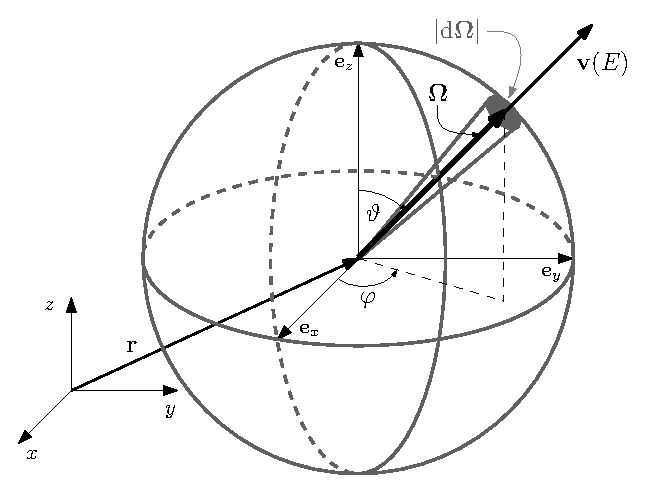
\includegraphics[scale=1]{phase_space.eps}
    \caption[Phase space of neutrons]{Phase space of neutrons}
    \label{fig:phase_space}
\end{figure}%
The product Lebesgue measure
\begin{equation}\label{eq:measure}
  \d{x} = \d{\mu(X)} = \d{\mu(V\times\Sphere\times [\Emin,\Emax])} = \d{\br}\d{\bomega}\d{E}
\end{equation}
is used when integrating over $X$, 
while the boundary measure
\begin{equation}\label{eq:measure2}
\db = \abs{\bomega\cdot\bn}\d{\gamma}\d{\bomega}\d{E},\quad \d{\gamma} = \d{\mu(\pV)},
\end{equation}
is used when integrating over $\pX[\pm]$. We note that because of the assumed regularity of the boundary, $\pX[0]$ is a
closed subset of $\pX$ of $\db$-measure zero (\cite[Chap. XXI, Sec. 2.2]{DautrayLions}). This will allow us to decompose
spaces of measurable functions defined on $\pX$ into a direct sum of subspaces of measurable functions defined on
$\pX[+]$ and $\pX[-]$, respectively. When refering to physical units, we will consider the length scale of $\VV$ in
centimeters.

\comment{
When discussing various semi-discretizations of the NTE, we will also refer to the following subspaces  (``sections''
through the phase space):
\begin{equation}\label{eq:pssec}
	X_E := \{(\br,\bomega,E):\ \br\in \VV\subset\R[3], \bomega\in \Sphere, E \in [\Emin,\Emax]\}
\end{equation}
}

Since the direction vectors are confined to the sphere, we can express the three
Cartesian components of $\bomega$ by only two spherical coordinates $\polar\in[0,\pi]$ and
$\azimuthal\in[0,2\pi)$\nomenclature[g]{$\polar$}{polar angle}\nomenclature[g]{$\azimuthal$}{azimuthal
angle}:
\begin{equation*}
	\bomega = \left[\begin{array}{c}
		\Omega_x \\
		\Omega_y \\
		\Omega_z
	\end{array}\right] = \left[\begin{array}{c}
		\sint\cosp \\
		\sint\sinp \\
		\cost
	\end{array}\right]
\end{equation*}
(see \fref{fig:streaming}).
\begin{figure}[!hbt]
    \centering
    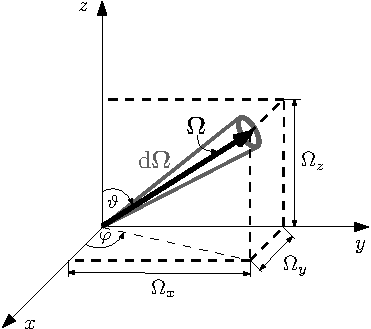
\includegraphics[scale=1.275]{cartesian_streaming}
    \caption[Cartesian coordinate system]{Cartesian coordinate system}
    \label{fig:streaming}
\end{figure}
To transform integrals with respect to $\d{\bomega}$ into double integrals with respect to $\polar$ and $\azimuthal$,
note that the solid angle $\d{\bomega}$ subtended at the center of $\Sphere$ by the spherical differential element
$\abs{\d{\bomega}}$ can be written as:
$$
	\d{\bomega} = \frac{\abs{\d{\bomega}}}{r^2} = \frac{r^2 \sint \d{\polar}\d{\azimuthal}}{r^2} =  \sint
	\d{\polar}\d{\azimuthal} $$
(see \fref{fig:element}).
\begin{figure}[!hbt]
    \centering
    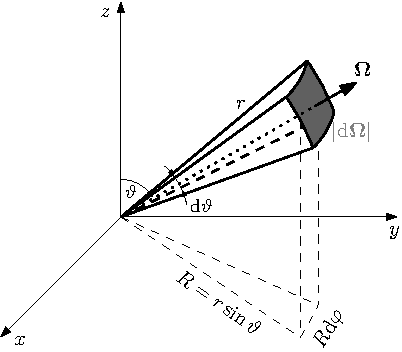
\includegraphics[scale=1.275]{element}
    \caption[Solid angle]{Schematic of the (scaled) solid angle of directions}
    \label{fig:element}
\end{figure}
We will also need to integrate functions that depend on the cosine of the angle between two 
directions $\bomega$ and $\bomega'$. We shall denote this angle and its cosine by $\polar_0$ and $\mu_0$, respectively
(see \fref{fig:scatter} in appendix for geometrical interpretation).
Then
$$
	\mu_0 \equiv \cos \polar_0 = \bomega\cdot\bomega'
$$
and
\begin{equation}\label{eq:invint}
\begin{aligned}
	\intA[']{f(\bomega\cdot\bomega')} &= \int_{0}^{2\pi} \int_{0}^{\pi}
		f(\cos \polar_0) \sin \polar_0\d{\polar_0} = 2\pi \muint[_0]{f(\mu_0)}\\
		&= \intA{f(\bomega'\cdot\bomega)}
\end{aligned}
\end{equation}
Notice that the result depends on neither $\bomega$ nor $\bomega'$.

\section{Steady state neutron transport in isotropic bounded domain}\label{sec:NTE}
In most practical cases, we can assume that the medium in which we study neutron transport is isotropic.
The first consequence of this assumption is that 
$$
	\sigma_t(\br,\bomega,E)\psi(\br,\bomega,E) \equiv \sigma_t(\br,E)\psi(\br,\bomega,E)
$$ 
for any $\bomega\in\Sphere$. The
second is that reactions that change the direction of neutrons from $\bomega'$ to $\bomega$ are
invariant under rotation of the coordinate system and are thus completely determined by the cosine of the two vectors:
\begin{equation}\label{eq:iso}
	\kappa(\cdot,\bomega\sla\bomega',\cdot) \equiv \kappa(\cdot,\bomega\cdot\bomega',\cdot).
\end{equation}
The steady state NTE \eqref{eq0} in this regime reads
\begin{equation}\label{eq1}
\begin{multlined}
  \bomega\cdot\nabla\psi(\br,\bomega,E) + \sigma_t(\br,E)\psi(\br,\bomega,E) =\\[.25em]
   = \intE[']{\Emin}{\Emax}{
      \intA[']{\kappa(\br,\bomega\cdot\bomega',E\sla E')\psi(\br,\bomega',E')}
    } + q(\br,\bomega,E)
 \end{multlined}
\end{equation}
in $X$, complemented by specified angular flux distribution at $\pX[-]$. The two prototypical inflow boundary
conditions are:
\begin{itemize}
	\item incoming angular neutron flux
	\begin{equation}\label{eq:nte2}
	  \psi\vert_{\pX[-]} = \psi_{\text{in}}
	\end{equation}
	($\psi_{\text{in}}\equiv 0$ corresponds to vacuum in $\R[3]\setminus \overline V$, which is a common
	 assumption in nuclear reactor modeling),
	
	\item albedo boundary reflection
	\begin{equation}\label{eq:nte3}
  	\psi(\br,\bomega,E) = \alpha(\br)\psi(\br, \bomega_R, E),\quad (\br,\bomega,E)\in \pX[-],\ \ \bomega_R = \bomega - 2
  	\bn (\bomega \cdot \bn)
  \end{equation}
  where $\bomega$ is the reflection of $\bomega_R$ about the boundary plane. For $\alpha \equiv 1$, this corresponds to
  complete specular reflection and is used to model planes of symmetry, while for $\alpha =
  0$, we recover the vacuum condition from above. Intermediate values mean that a fraction of neutrons leaving the
  domain in direction $\bomega_R$ are returned back in direction $\bomega$, which is commonly used to model reactor
  reflectors. We thus assume $0 \leq \alpha \leq 1$. 
\end{itemize}
\begin{remark}
	The albedo coefficient $\alpha$ may in general vary with the reflector properties and should also capture 
	redistribution of the reflected neutrons within the phase space due to their diffusion through the reflector. A general
	treatment of albedo condition is given in \cite{Sanchez4} (see also \cite{Sanchez3}), where an integral albedo operator
	$\beta$ is introduced, such that
\begin{equation}\label{eq:albedo-general}
	\angflux(x)\big\vert_{\pX[-]} = (\beta\angflux)(x) = \bndint[']{\pX[+]}\beta(x\sla x')\angflux(x'),
\end{equation}
	where $x = (\br,\bomega,E)$ and $x' = (\br',\bomega',E')$. 
\end{remark}
For formal description of other types of boundary conditions, we refer to \cite{Sanchez4} or \cite[Sec. 1.3]{Agoshkov}.

A physically plausible solution of NTE should be moreover non-negative throughout $\VV$ and continuous along any
direction $\bomega$, i.e. $\psi(\br + s\bomega,\bomega,E)$ is a continuous function of $s$ for any $\br$, $\bomega$, $E$. Note
that $\psi(\br + s\bomega',\bomega,E)$ \textsl{may} be discontinuous when $\bomega' \neq \bomega$.

\subsection{Advection term}\label{sec:advection}
In Cartesian coordinate system (that we will exclusively consider in this thesis),
$$
	\bomega\cdot\nabla\angflux = \bomega_x\pd{\angflux}{x} + \bomega_y\pd{\angflux}{y} + \bomega_z\pd{\angflux}{z} = 
	\der{x}{s}\pd{\angflux}{x} + \der{y}{s}\pd{\angflux}{y} + \der{z}{s}\pd{\angflux}{z} = \der{\angflux}{s},
$$
where $s\in I\subset \R$ parametrizes the path traveled by the neutron along the direction $\bomega$ (the
\textit{characteristic}, see \fref{fig:cartesian2}).
\begin{figure}[htp]
\begin{center}
  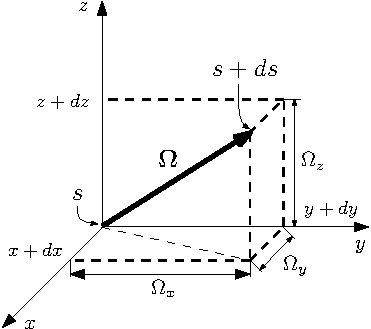
\includegraphics[scale=1.2]{cartesian_streaming2}
  \caption{Characteristic direction in the Cartesian coordinate system}
  \label{fig:cartesian2}
\end{center}
\end{figure}
Assuming now for simplicity that the integral term on the right of \eqref{eq1} is absorbed in the source term $q$, we
may invert the differential operator on the left of \eqref{eq1} by integration along these characteristics and obtain an
integral formulation of the neutron transport equation:
\begin{equation}\label{eq:nte-integral}
	\angflux(\br,\bomega) = \angflux(\br_0,\bomega)e^{-\tau(\br,\br_0)} + \int_0^{s_0}
	q(\br',\bomega)e^{-\tau(\br,\br')}\,\d{s'}
\end{equation}
where
\begin{align}
	\br' &= \br - s' \bomega, \quad \br_0 = \br - s_0 \bomega\nonumber\\[.2em]
	\tau(\br,\br') &= \tau(\br,\br-s'\bomega) = \int_0^{s'} \sigma_t(\br - s''\bomega)\,\d{s''} \label{eq:tau}
\end{align}
In reference to \fref{fig:trepka}
\begin{figure}[htp]
\begin{center}
  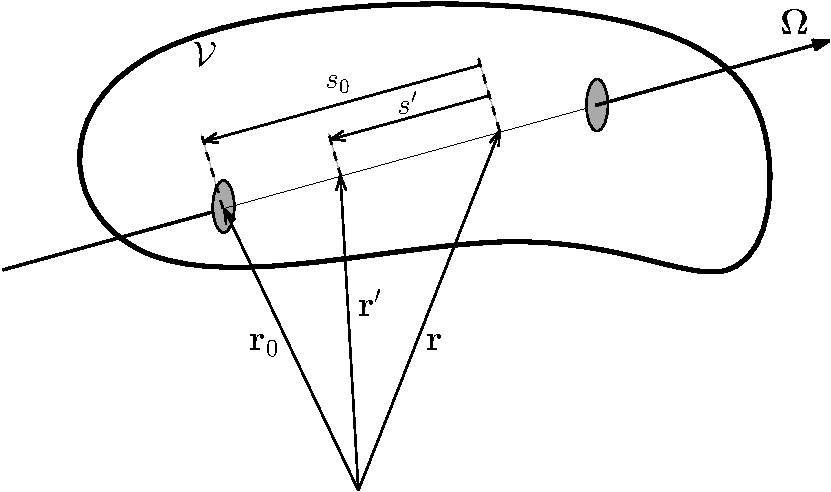
\includegraphics[scale=.75]{trepka}
  \caption{Illustration for the solution on a characteristic}
  \label{fig:trepka}
\end{center}
\end{figure}
we can interpret the first term on the right of \eqref{eq:nte-integral} as the number of
neutrons moving in the direction $\bomega$ that entered the given volume in $\br_0$ and reached point $\br$ without
collision, whereas the second term as the number of neutrons introduced into the characteristic direction by sources 
between $\br_0$ and $\br$ and reaching $\br$ without collision. The \textit{optical path length} $\tau$ represents the 
probability of collision between $r'$ and $r$. This integral form is of both theoretical and practical value, as we will
see later in sections \ref{sec:fixed-source} and \ref{sec:lattice}.

\subsection{Collision terms}
The kernel of the integral operator on the right-hand side of \eqref{eq1} can be split into the so-called
\textit{double-differential macroscopic cross-section} for scattering and fission, respectively:
\begin{equation}\label{eq:splitting}
  \kappa(\br,\bomega\cdot\bomega',E\sla E') = \sigma_s(\br,\bomega\cdot\bomega',E\sla E') +
  \sigma_f(\br,\bomega\cdot\bomega',E\sla E').
\end{equation}
These cross-sections characterize the mean number of ($\bomega$, $E$)-neutrons coming out of a (possible) collision of 
($\bomega'$, $E'$)-neutrons with nuclei at $\br$ (or more precisely in a
differential element around $\br$). Such collisions can either just change the direction and energy of the
inducing neutrons (elastic scattering) or cause absorption of the neutrons followed by release of
new ones in the considered direction and energy range (fission), or both (inelastic scattering).
Ordinary macroscopic cross-sections $\sigma_s(\br,E)$, $\sigma_f(\br,E)$ are then introduced to characterize the total
probability that $(\bomega,E)$ neutrons undergo collisions of the above type irrespective of the outgoing direction and
energy\footnote{Recall that the direction $\bomega$ of the incoming neutrons is irrelevant for the result as a
consequence of the assumption of isotropic medium (and eq. \eqref{eq:invint}).}, i.e.
\begin{equation}\label{eq:ddifxs}
\begin{aligned}
\eta\sigma_s(\br, E) &=
\intE[']{\Emin}{\Emax}{\intA[']{\sigma_s(\br,\bomega'\cdot\bomega, E'\sla E)}},\\
\nu\sigma_f(\br, E) &= \intE[']{\Emin}{\Emax}{\intA[']{\sigma_f(\br,\bomega'\cdot\bomega, 
	E'\sla E)}}
\end{aligned}
\end{equation}
where $\eta$ and $\nu$, respectively, are the expected number of neutrons coming out of the scattering event ($=1$ in
case of elastic scattering, might be $> 1$ when inelastic scattering takes place) and the fission event, respectively. 

The \textit{total macroscopic cross-section}, $\sigma_t$, characterizing the probability that neutron with energy $E$
undergoes a collision of any type with nuclei at $\br$, can now be decomposed as 
\begin{equation}\label{eq:st}
  \sigma_t(\br,E) = \sigma_c(\br,E) + \sigma_f(\br,E) + \sigma_s(\br,E) \equiv \sigma_a(\br,E) + \sigma_s(\br,E)
\end{equation}
where
\begin{itemize}
	\item $\sigma_c(\br, E)$ is the non-productive capture cross section (resulting in no new neutrons being introduced
	into the system) and
  	\item $\sigma_a(\br, E) = \sigma_c(\br,E) + \sigma_f(\br,E)$ is the absorption cross section.
\end{itemize}

For later use, note that fission is an isotropic process (which removes the angular dependence of the
double-differential fission cross-section altogether) and the new energy distribution does not depend on the energy of 
the inducing neutron 
\begin{figure}[hbt]
\begin{center}
  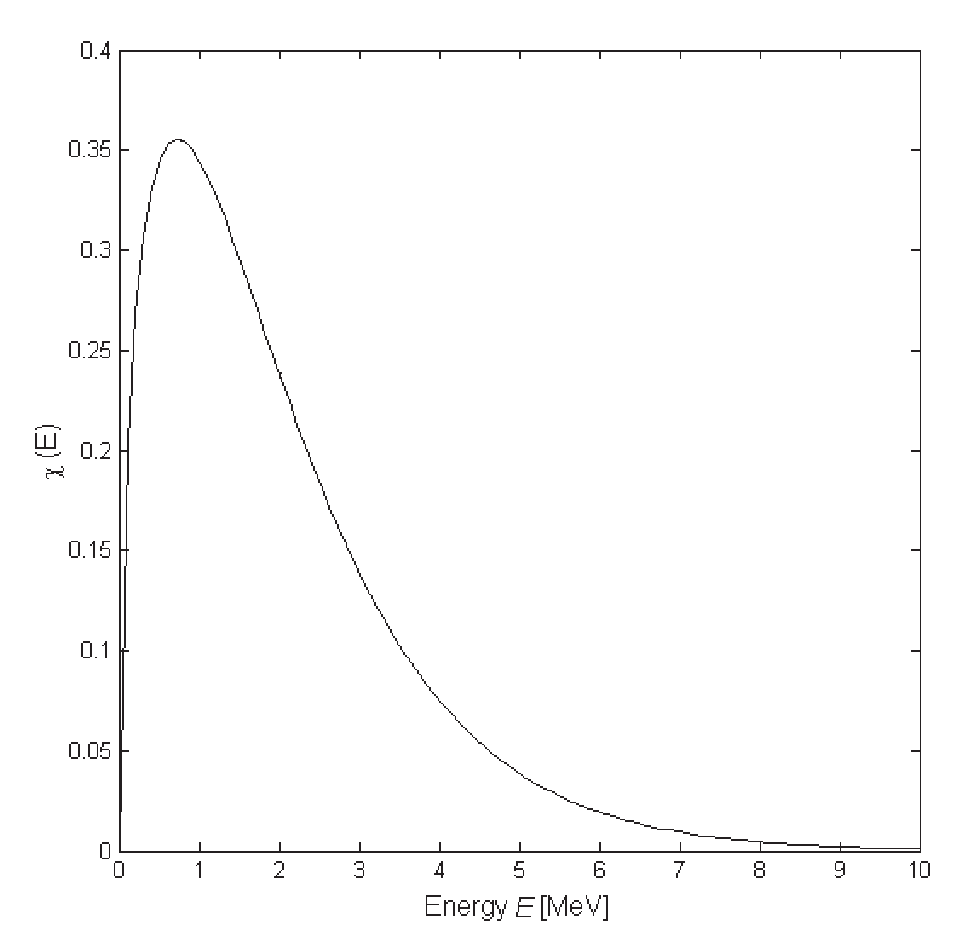
\includegraphics[scale=.6]{spectrum}
  \caption{Energy spectrum of (prompt) neutrons released from fission of U235}
  \label{fig:spectrum}
\end{center}
\end{figure}
(as it corresponds to the neutrons originally bound inside the nucleus; \fref{fig:spectrum}
shows a typical shape of that function); using the second eq.
\eqref{eq:ddifxs}, we can then write:
\begin{equation}\label{eq:sf}
\sigma_f(\br,\bomega\cdot\bomega',E\sla E') = \frac{\chi(E)\nu\sigma_f(\br,E')}{4\pi},\quad 
\intE{\Emin}{\Emax}{\chi(E)} = 1.
\end{equation}
 
A physically realistic assumption is that all the macroscopic cross-sections are bounded measurable functions
\footnote{with respect to product measure of type \eqref{eq:measure} appropriate for their particular set of arguments,
 or with respect to $\d{\mu(V\times\Sphere^2\times [\Emin,\Emax]^2)}$ in case of double-differential cross-section},
 piecewise continuous in $\VV$. The unit of macroscopic cross-sections is \SI{}{cm^{-1}}.

\subsection{Quantities of interest}\label{sec:qoi}
From the solution of eq. \eqref{eq1}, one can derive the following important integral quantities
\begin{itemize}
  \item \textit{scalar neutron flux density} \SI{}{[cm^{-2}.s^{-1}]}
  \begin{equation}\label{eq:scalar_flux}
    \phi(\br, E) = \intA{\psi(\br,\bomega,E)},
  \end{equation}
  \item \textit{net neutron current density} \SI{}{[cm^{-2}.s^{-1}]}
	\begin{equation}\label{eq:bJ}
		\bJ(\br, E)	= \intA{\bomega\psi(\br,\bomega,E)},
	\end{equation}
\end{itemize}
so that integrating $\bJ(\br,E)\cdot\bn(\br)$ over a given surface 
gives the total number of neutrons with energy $E$ crossing (per unit time) that surface in the direction of 
$\bn$ (and allows us to assess neutron conservation within given volume, recall Remark \ref{rem:balance}).

The integral
\begin{equation}\label{eq:rr}
  \intE{E_1}{E_2}{\sigma_x(\br, E) \phi(\br, E)}
\end{equation}
represents the \textit{reaction rate density} (per unit time) ou viven type ($x = t,a,f,s,c$, see \eqref{eq:st}), 
induced by neutrons of energies in range $[E_1, E_2]$. 
As well as the scalar flux itself, reaction rates may be experimentally measured
by various detector mechanisms, which is the reason why these quantities are more important in practical calculations
than the actual solution of the NTE (the angular neutron flux). Of particular importance for reactor calculations is the
\textit{power density} 
\begin{equation}\label{eq:power}
	P(\br) = \intE{\Emin}{\Emax}{e\sigma_f(\br, E) \phi(\br, E)} \quad \SI{}{[W.cm^{-3}]}
\end{equation}
where $e$ is the energy conversion factor converting fission rate to watts.

\subsection{Solvability of neutron transport problems}\label{sec:ntp}
In this section, we will formulate the two basic problems of neutron transport in an operator form.
We will consider the generalized statements in which the equation and boundary conditions are assumed to be
satisfied a.e. in $X$ and $\bomega\cdot\nabla$ represents the generalized derivative in the usual Sobolev sense. This is motivated by the low
regularity that can be expected from the exact solution of the NTE -- for example, even for piecewise smooth material data
(cross-sections $\sigma_x$) and sources $q$, the solution of the NTE is known to possibly exhibit singularities in 
first partial derivatives (or be discontinuous as a function of $\bomega$) at surfaces of material discontinuities 
coinciding with characteristic curves of the left-hand side of \eqref{eq1} (that is, straight lines; see \cite[Chap.
1]{Agoshkov}, \cite[Sec. III]{Vladimirov}). We will call the solution of such a generalized problem a \textit{weak
solution}.



\subsection{Neutron transport problem with fixed sources}\label{sec:fixed-source}
Let us introduce the standard spaces of Lebesgue-integrable functions (w.r.t. the product measure \eqref{eq:measure},
resp. \eqref{eq:measure2}) 
\begin{equation}\label{eq:Lp}
\nomenclature[a]{$\Lp(X)$}{space of functions integrable in the Lebesgue sense with their $p$-th power over
$X$\nomrefeq}
\nomenclature[a]{$\Lp_\sigma(X)$}{space weighted with the total cross-section $\sigma_t$\nomrefeq}
\begin{aligned}
	\Lp(X) &= \left\{\psi\mid \norm[\Lp(X)]{\psi} := \left(\int_X\abs{\psi(x)}^p\,\d{x}\right)^{1/p} <
	\infty\right\},\quad 1\leq p < \infty,\\
	\Lp(\pX[\pm]) &= \left\{\psi\mid \Vert\psi\Vert_{\Lp(\pX[\pm])} :=
	\left(\int_{\pX[\pm]}\abs{\psi(x)}^p\,\db\right)^{1/p} < \infty\right\},\quad 1\leq p < \infty,\\
	\Lp[\infty](X) &= \{\psi\mid \norm[L^{\infty}(X)]{\psi} := \esssup_{X} \abs{\psi(x)} < \infty\}\\
	\Lp[\infty](\pX[\pm]) &= \{\psi\mid \Vert\psi\Vert_{L^{\infty}(\pX[\pm])} := \esssup_{\pX[\pm]}
	\abs{(\bomega\cdot\bn)\psi(x)}< \infty\}
\end{aligned}
\end{equation}
Note that for the total volumetric scalar flux to be finite  (as is physically expected), the solution should belong to
$\Lp[1](X)$.
\index{$\Lp(X)$}\index{$\Lp[\infty](X)$}\index{\Lp(\pX[\pm])}\index{\Lp[\infty](\pX[\pm])}

We formulate the fixed source problem using the following operators:
\begin{equation*}
  \begin{gathered}
    A\psi(\br,\bomega,E) = \bomega\cdot\nabla\psi(\br,\bomega,E),\\%[.85em]
    \Sigma_t\psi(\br,\bomega,E) = \sigma_t(\br,E)\psi(\br,\bomega,E),\\%[.75em]
    K\psi(\br,\bomega,E) = \intE[']{\Emin}{\Emax}{
            \intA[']{\kappa(\br,\bomega\cdot\bomega',E\sla E')\psi(\br,\bomega',E')}
          }.
  \end{gathered}
\end{equation*}
We shall call $A$, $\Sigma_t$, $K$ and $T = A + \Sigma_t - K$ the \textit{advection}, \textit{reaction}, 
\textit{collision} and \textit{transport} operator, respectively. All these operators are continuous; the reaction
operator $\Sigma_t : \Lp(X) \to \Lp(X)$ is a simple multiplication operator in $\Lp(X)$, self-adjoint and bounded,
while the operator $K: \Lp(X) \to \Lp(X)$ is bounded under additional (physically justifiable) conditions
(e.g. conditions (c) and/or (d) of the following theorem, depending on the chosen $p$), but is self-adjoint if and only 
if the kernel $\kappa$ of $K$ is symmetric in $E$ and $E'$. With the exception of the mono-energetic case, this is
generally not true (a fact to which we return again in \sref{sec:MG}). To further simplify notation, let us also define 
$$
	\op{L} := A + \Sigma_t.
$$
\index{$\op{L}$}\index{$A$}\index{$\Sigma_t$}\index{$K (operator)$}%
For piecewise smooth
$\pV$ and $1\leq p < \infty$, the traces $\gamma_{\pm}\psi \equiv \psi\vert_{\pX[\pm]}\in\Lp(\pX[\pm])$ are well defined
for functions $\psi\in \widehat H^p(X)$, where
$$
\widehat H^p(X) = \{\psi\mid \psi\in\Lp(X), \bomega\cdot\nabla\psi\in\Lp(X)\}, \quad 1 \leq p \leq \infty
$$
and a continuous lifting operator 
$$
	\mathcal{G}: \psi_{\pm}\in\Lp(\pX[\pm]) \mapsto \widehat\psi \in \widehat H^p(X)
$$
such that $\widehat\psi\vert_{\pX[\pm]} = \psi_{\pm}$ exists (\cite[Thm. 1, Appendix of \S 2, Chap.
XXI]{DautrayLions}, \cite{Boulanouar1} for the case $p = \infty$).
Let us then define the Sobolev space of functions with bounded boundary traces
\begin{equation}\label{eq:Hp}
  \nomenclature[a]{$\Hp{p}(X)$}{Sobolev space of functions whose (generalized) partial derivatives up to order $k$ are
 in $\Lp{p}$.\nomrefeq} 
 \Hp(X) := \left\{\psi\in\Lp(X), \bomega\cdot\nabla\psi\in\Lp(X), \Vert\gamma\psi\Vert_{\Lp(\pX)} < \infty\right\}. 
\end{equation}
\index{\Hp(X)}%
We note that $\Hp[2](X)$ is a Hilbert space when equipped with the inner product
\begin{equation*}\label{eq:ip}
	\ip{\Hp[2](X)}{\psi,\varphi} := \ip{\Lp[2](X)}{\bomega\cdot\nabla \psi, \bomega\cdot\nabla \varphi} +
	\ip{\Lp[2](X)}{\psi,\varphi} +
	\ip{\Lp[2](\pX)}{\psi,\varphi} 	
\end{equation*}
where
\begin{equation}\label{eq:ipL2}
	\ip{\Lp[2](X)}{\psi,\varphi} = \int_X \psi \varphi \,\d{x},\quad
	\ip{\Lp[2](\pX)}{\psi,\varphi} = \int_{\pX} \psi \varphi \,\d{\xi}.
\end{equation}
\index{$\ip{\Hp[2](X)}{\cdot,\cdot}$}\index{$\ip{\Lp[2](X)}{\cdot,\cdot}$}

\begin{remark}\label{rem:lifting}
The lifting operator allows us to pick a function $\widehat \psi = \mathcal{G}\psi_{\text{in}} \in \Hp(X)$ and convert a
problem $T\psi = q$ with non-homogeneous boundary conditions \eqref{eq:nte2} to a problem 
$$
	T(\psi - \widehat\psi) = q - T\widehat\psi \equiv \widehat q
$$ 
where trace of the new unknown function $u = \psi - \widehat\psi$ on $\pX[-]$ vanishes. Final solution is then recovered
as $\psi = u + \widehat{q}$. Therefore, we can focus on the case with homogeneous conditions. Results for the reflective or more general
boundary conditions require special trace theorems, see \cite[Chap. XXI, Appendix of \S2]{DautrayLions} or \cite[Chap. 2]{Agoshkov} 
\end{remark}

The fixed source, steady state neutron transport problem with vacuum boundary conditions that we are going to study in
this section is posed as follows

\begin{problem}\label{prb:1}
For given $q\in \Lp(X)$ find $\psi \in \Dom{T} \subset \Lp(X)$ such that
$$
  \left\{
  \begin{aligned}
     &T\psi(\br,\bomega,E) = q(\br,\bomega,E),\\
     &\Dom{T} = \{\psi\in \Hp(X),\ \psi\vert_{\pX[-]} = 0\},
  \end{aligned}
  \right.
$$
\end{problem}

We will first consider the physically most natural $\Lp[1](X)$ setting.

\subsubsection{$\Lp[1](X)$ setting}
\begin{theorem}\label{thm1}
Assume that
\begin{enumerate}[label=(\alph*)]
	\item $\sigma_t \in \Lp[\infty](X)$, $\sigma_t \geq \mst > 0$ a.e. in $\VV\times[\Emin,\Emax]$,
	\item $\kappa \geq 0$ a.e. in $\VV\times\Sphere^2\times[\Emin,\Emax]^2$,
	\item $\displaystyle c \leq \bar c < 1$ a.e. in $\VV\times[\Emin,\Emax]$ where
	  \begin{equation}\label{eq:c}
	    c(\br,E) := \frac{1}{\sigma_t(\br,E)}\int_{\Emin}^{\Emax}\int_{\Sphere} \kappa(\br,\bomega'\cdot\bomega,
	    E'\sla E)\,\d{E'}\d{\bomega'}.
	  \end{equation}
\end{enumerate}
Then Problem \ref{prb:1} with $p = 1$ has for any $q\in \Lp[1](X)$ a unique weak solution 
$\psi(\br,\bomega,E)\in\Dom{T}\subset\Lp[1](X)$.
\end{theorem}
\begin{proof}
\cite[Chap. XXI, \S 2, Proposition 5]{DautrayLions}
\end{proof}

The value $c$ in Thm. \ref{thm1} has the physical meaning of the mean (net) number of neutrons emitted (in all possible
directions and energies) per a neutron with energy $E$ (coming from any direction) colliding with a nucleus at point
$\br\in V$. 
Condition (c) thus expresses the requirement that the system be \textit{subcritical} in order for a
steady solution in presence of external sources to be achieved (the notion of criticality will be formally introduced in the following
subsection).
Notice that (using \eqref{eq:ddifxs})
\begin{equation}\label{eq:scattering_ratio}
	c(\br,E) = \frac{\eta\sigma_s(\br,E) + \nu\sigma_f(\br,E)}{\sigma_t(\br,E)}
\end{equation}
and is usually called \textit{collision ratio} \index{c|see{collision ratio}}\index{collision ratio} (or
\textit{scattering ratio} in non-fissioning domains)\index{scattering ratio}.

 In \cite{Sanchez3}, Sanchez uses the inversion of the transport operator along characteristics (see \ref{sec:advection}
 above) to prove existence and uniqueness of a solution to the fixed source neutron transport problem in
 the cross-section weighted space $\Hp[1]_{\sigma}(X)$ for right hand sides in $\Lp[1]_{\sigma}(X)$.
 This appears to be an alternative physically natural functional setting due to the definition of the reaction rate, eq. 
 \eqref{eq:rr}; moreover, assumption (a) may be relaxed by allowing $\sigma_t = 0$ in arbitrarily large regions 
  (the \textit{void regions}). Note that if we assume (a) of Thm. \ref{thm1}, the norms of $\Lp[1]$ and
  $\Lp[1]_{\sigma}$ are equivalent and the measure $\d{\tau} = \sigma_t(x) \d{x}$ associated with the space
  $\Lp[1]_{\sigma}$ represents a differential optical path length (see eq. \eqref{eq:tau}).

\subsubsection{$\Lp[\infty](X)$ setting}
In \cite[Chap. XXI, \S 2, Proposition 6]{DautrayLions}, Dautray and Lions also 
show the existence of unique solution in $\Lp[\infty](X)$ for $q\in \Lp[\infty](X)$; the proof in this case is again
based on the inversion of the transport operator along characteristics and requires instead of
 (c) the condition
\begin{enumerate}
  \item[(d)] $d \leq \bar d < 1$ a.e. in $\VV\times[\Emin,\Emax]$
\end{enumerate}
where
\begin{equation}\label{eq:d} 
d(\br,E) := 
  \frac{1}{\sigma_t(\br,E)}\int_{\Emin}^{\Emax}\int_{\Sphere} \kappa(\br,\bomega\cdot\bomega',
	    E\sla E')\,\d{E'}\d{\bomega'}
\end{equation}
can be interpreted as the average number of neutrons emitted with energy $E$ (into any direction) from
collisions induced by all possible neutrons impinging on the nucleus at $\br$ (again, this is a reasonable condition
in the subcritical state). Notice that because angular dependence of $\kappa$ is only through the cosine of the
collision angle ($\bomega\cdot\bomega'$), assumptions (c) and (d) really represent different assumptions about just the energy
transfer in collisions. 

\subsubsection{$\Lp[2](X)$ setting and second-order forms of NTE}\label{sec:L2}
In general $\Lp(X)$ spaces with $1 < p < \infty$, Dautray and Lions outline the proof based on the same ideas as those 
used in the $\Lp[1](X)$ case (theory of monotone operators), utilizing assumptions (a-d) of Thm. \ref{thm1}.  The case
$p = 2$ is particularly important\footnote{even though it does not lead to a direct physical interpretation as  the
$\Lp[1](X)$ setting} as the Hilbert space structure of $\Lp[2](X)$ allows to use richer set of mathematical tools to 
formulate practical solution methods. It also allows to formulate variational principles for the NTE, in the spirit of 
the seminal work of Vladimirov \cite{Vladimirov}. This approach allows to find the weak solution of the neutron 
transport problem $$
\begin{aligned}
     &T\psi(\br,\bomega,E) = q(\br,\bomega,E),\\
     &\Dom{T} = \{\psi\in \Hp[2](X),\ \psi\vert_{\pX[-]} = 0\},
  \end{aligned}
$$
by solving an equivalent weak problem of finding $\psi\in\Hp[2](X)$ such that
\begin{equation}\label{eq:weakform}
	\langle \tilde{T}\psi, \varphi \rangle = \langle \tilde{q}, \varphi \rangle  \quad \forall \varphi\in \Hp[2](X),
\end{equation}
with $\tilde{T}$ being a bounded and coercive operator on $\Hp[2](X)$ ($\langle \cdot,\cdot\rangle$ denotes the
duality pairing between $\Hp[2](X)$ and the dual space of bounded linear functionals on $\Hp[2](X)$; if we consider
$\tilde{T} : \Hp[2](X) \to \Lp[2](X)$ and $q\in \Lp[2](X)$, this pairing coincides with the standard $\Lp[2](X)$ inner
product \eqref{eq:ipL2}). Well-posedness of this problem is then an immediate consequence of the Lax-Milgram lemma. 

Bourhrara formulates in \cite{Bourhrara2} three such principles for the fixed source problem (and one for the
criticality problem investigated in the following section) and shows that some of these formulations could be obtained
also as weak forms of the traditional second-order forms of the transport equation -- the even parity equation (obtained
by writing eq.
\eqref{eq1} for $\bomega$ and $-\bomega$, adding and subtracting the two resulting equations and eliminating the
unknowns of odd parity) and the self-adjoint angular flux equation (obtained by
expressing $\psi$ from the $\sigma_t\psi$ term of \eqref{eq1} in terms of the remaining terms and substituting back into
the advection term). He also provides a comparison with other formulations based on the least-squares approach
(minimizing the appropriately scaled residual \mbox{$\norm[{\Lp[2](X)}]{\mathcal{P}(\tilde T \psi - q)}^2 +
\varpi\norm[{\Lp[2](\pX[-])}]{\psi_{\text{in}} - \psi}^2$}) studied e.g. in \cite{Manteuffel} or
\cite{Agoshkov}. 

Approximations of eq. \eqref{eq:weakform} leading to numerical solution methods are naturally obtained by restricting
the formulation to finite-dimensional subspaces of $\Hp[2](X)$. With bounded and coercive $\tilde T$, approximation
error is then automatically provided by the C{\' e}a lemma. In the angular domain, this has
been done using the subspace of spherical harmonics of finite degree in \cite{bourhrara3} of \cite{Manteuffel}, which
is also known as the $\PN$ method. As we will see in \sref{sec:1-SN}, this can be done also with the other most widely 
employed angular approximation methods, the $\SN$ method of discrete ordinates.

\comment{ We will now take yet another approach and prove the
existence and uniqueness in $\Lp[2](X)$ using the contraction principle (\cite[Thm. 2.3.1]{DrabekNFA}). As we will see
in the following chapter, the results from next subsection will have direct consequences for the numerical solution methods for the NTE.

\subsubsection{$\Lp[2](X)$ setting}\label{sec:L2}

Let us start by stating some well-known results that hold in the $\Hp[2](X)$.
This is a Hilbert space when equipped with the inner product
$$
	\ip{\Hp[2](X)}{\psi,\varphi} := \ip{\Lp[2](X)}{\bomega\cdot\nabla \psi, \bomega\cdot\nabla \varphi} +
	\ip{\Lp[2](X)}{\psi,\varphi} +
	\ip{\Lp[2](\pX)}{\psi,\varphi} 
$$
where
\begin{equation}\label{eq:ipL2}
	\ip{\Lp[2](X)}{\psi,\varphi} = \int_X \psi \varphi \,\d{x},\quad
	\ip{\Lp[2](\pX)}{\psi,\varphi} = \int_{\pX} \psi \varphi \,\d{\xi}.
\end{equation}
Let us denote 
\begin{equation}\label{eq:opL}
	\op{L} := A + \Sigma_t.
\end{equation}
Using the Poincar{\' e}-Friedrichs inequality and integration by parts (see e.g. \cite[Chap.
2]{Agoshkov}), one can show the following:
\begin{lemma}\label{lem:Lcoercive}
	Assume (as in item (a) in Thm. \ref{thm1}) that 
	$$
		0 < \mst \leq \sigma_t \leq \Mst \ \text{a.e. in } \VV\times[\Emin,\Emax].
	$$
	Then the operator $\op{L} : \Hp[2](X) \to \Lp[2](X)$ is
	bounded and coercive with constants $\Mst$ and $\mst$, respectively: 
	$$
		\ip{\Lp[2](X)}{L\psi, \psi} \geq \mst \norm[{\Hp[2](X)}]{\psi}^2,\quad  \norm[{\Lp[2](X)}]{L\psi} \leq \Mst
		\norm[{\Hp[2](X)}]{\psi}^2.
	$$
\end{lemma}
Also, as a consequence of H\"older inequality, the collision operator
\linebreak[4]\mbox{$\op{K} :
\Lp[2](X) \to \Lp[2](X)$} is bounded (this is a special case of \cite[Lemma 1, \S 3, Chap. XXI]{DautrayLions} for $p =
2$):
\begin{lemma}\label{lem:Kbounded}
	Assume that there exist $M_a > 0$, $M_b > 0$, such that for a.e. $(\br,E) \in \VV\times[\Emin,\Emax]$
	$$
	\begin{aligned}
	&\int_{\Emin}^{\Emax}\int_{\Sphere} \kappa(\br,\bomega\cdot\bomega',
	    E'\sla E)\,\d{E'}\d{\bomega'} \leq M_a,\\
	&\int_{\Emin}^{\Emax}\int_{\Sphere} \kappa(\br,\bomega\cdot\bomega',
	    E\sla E')\,\d{E'}\d{\bomega'} \leq M_b.    
	\end{aligned}
	$$
	Then 
	$$
	\norm[{\Lp[2](X)}]{K\psi} \leq M_a^{\frac12} M_b^{\frac12} \norm[{\Lp[2](X)}]{\psi}.
	$$
\end{lemma}

We will now use these results to show the existence and uniqueness of a weak solution to the steady state neutron
transport problem in $\Lp[2](X)$. For this we will utilize the famous Lax-Milgram lemma, which we now state in its
general form for an operator $\genop{A}$ being an element of space $\mathcal{L}(V,V')$ of bounded linear operators acting from 
a Hilbert space $V$ to its dual $V'$ \footnote{In general, we will denote by
$\mathcal{L}(V,W)$
\index{$\mathcal{L}(V,W)$} the Banach space of bounded linear operators mapping Banach space $V$ to a Banach space $W$ 
with norm $\norm[\mathcal{L}(V,W)]{\genop{A}} = \sup_{\norm[V]{v}=1} \norm[W]{\genop{A}v}$.} equipped with norm
$\norm[V']{f} = \sup_{\norm[V]{v} = 1} \abs{\langle f,v \rangle}$ ($\langle \cdot,\cdot\rangle$ being the duality 
pairing between $V$ and $V'$). Here and below, we use letters $u$, $v$ to denote general members of some vector space
$V$; this should not cause confusion, as $v$ with its other meaning of neutron's speed will never be used in the same
context.

\begin{lemma}[Lax-Milgram]\label{lem:lax-milgram}
	Let $\genop{A}\in\mathcal{L}(V,V')$ be a bounded and coercive operator with constants $C_b$ and $C_c$, respectively.
	Then for any $f\in V'$, there exists a unique $u\in V$ such that
	\begin{equation}\label{eq:laxmilgram}
		\langle \genop{A}u, v \rangle = \langle f, v \rangle  \quad \forall v\in V,
	\end{equation}
	and
	$$
		\norm[V]{u} \leq \frac{1}{C_c}\norm[V']{f}.
	$$
\end{lemma}
As usual, we will call eq. \eqref{eq:laxmilgram} a weak form of the operator equation $\genop{A}u = f$.
%We only note that considering $T:V\toV'$ (thus allowing more general right-hand sides) is possible, but we don't go into details here.

Lax-Milgram lemma allows us to prove the following lemma.
\begin{lemma}
	Let $\genop{A}\in\mathcal{L}(V,V')$ be bounded and coercive with constant $C_c$
	and let $\genop{F}:V\to V'$ be Lipschitz with constant $C_L$, i.e. 
	$$
		\exists C_L > 0: \norm[V']{\mathcal{F}v_1 - \mathcal{F}v_2} \leq C_L \norm[V]{v_1 - v_2}\quad \forall v_1,v_2 \in V. 
	$$
	If
	$$
		\frac{C_L}{C_c} < 1
	$$
	then the mapping $\mathcal{T} : v\in V \mapsto \mathcal{T}v\in V$ defined by solving
	$$
		\langle\genop{A}\mathcal{T}v, w\rangle = \langle \genop{F}v, w \rangle\quad \forall w \in V 
	$$
	is contraction.
\end{lemma}
\begin{proof}
	By Lax-Milgram lemma, the mapping $\mathcal{T}$ is well defined. For any $v_1,v_2\in V$, coercivity and
	linearity of $\genop{A}$, definition of $\genop{T}$ and Lipschitz property of $\genop{F}$ yields 
	$$
	\begin{aligned}
		C_c \norm[V]{\mathcal{T}v_1 - \mathcal{T}v_2}^2 &\leq 
		\langle \genop{A}\mathcal{T}v_1 - \genop{A}\mathcal{T}v_2, \mathcal{T}v_1 - \mathcal{T}v_2 \rangle \\
		& = \langle \genop{F}v_1 - \genop{F}v_2,  \mathcal{T}v_1 - \mathcal{T}v_2 \rangle \\
		& \leq \norm[V']{\mathcal{F}v_1 - \mathcal{F}v_2} \norm[V]{\mathcal{T}v_1 - \mathcal{T}v_2}\\
		& \leq C_L \norm[V]{v_1 - v_2} \norm[V]{\mathcal{T}v_1 - \mathcal{T}v_2}.
	\end{aligned}
	$$
	Therefore
	$$
		\norm[V]{\mathcal{T}v_1 - \mathcal{T}v_2}^2 \leq \frac{C_L}{C_c}\norm[V]{v_1 - v_2} 
	$$ 
	for arbitrary $v_1, v_2\in V$, proving the claim.
\end{proof}
As an immediate corollary, we obtain from the contraction principle
\begin{corollary}
	Let 
	$$
		\rho := \frac{C_L}{C_c} < 1.
	$$
	For any $u_{(0)} \in V$, the sequence of iterates $\{u_{(i)}\}_{i=1}^{\infty}$ of the iteration
	$$
		\langle\genop{A}u_{(i+1)},w\rangle = \langle \genop{F}u_{(i)}, w\rangle\quad \forall w \in V,\ \quad i = 0,1,\ldots
	$$
	converges to the unique fixed point $u^*$ of the mapping $u\in V \mapsto \genop{A}^{-1}\genop{F}u \in V$. Moreover, 
	$$
		\norm{u_{(i)} - u^*} \leq \frac{\rho^{i}}{1-\rho} \norm{u_{(1)} - u_{(0)}},\quad
		\norm{u_{(i)} - u^*} \leq \frac{\rho}{1-\rho} \norm{u_{(i)} - u_{(i-1)}}.
	$$   
\end{corollary}

In our case, $V = \Hp[2](X)$, $\genop{A} \equiv T : \Hp[2](X) \to \Lp[2](X) \subset V'$ and the duality pairing
$\langle \cdot,\cdot\rangle$ coincides with the $\Lp[2](X)$ inner product \eqref{eq:ipL2}.


We are now ready to prove the existence and uniqueness result.
\begin{theorem}
	Let the assumptions (a-d) of Theorem \ref{thm1} be satisfied.
	Then the fixed source, steady state neutron transport problem with vacuum boundary conditions 
\begin{equation*}
  \left\{
  \begin{aligned}
     &T\psi(\br,\bomega,E) = q(\br,\bomega,E),\\
     &\Dom{T} = \{\psi\in \Hp[2](X),\ \psi\vert_{\pX[-]} = 0\},
  \end{aligned}
  \right.
\end{equation*}
has a unique weak solution $\psi(\br,\bomega,E)\in\Dom{T}\subset\Lp[2](X)$ for any $q\in \Lp[2](X)$.
\end{theorem}
\begin{proof}
	It follows from \eqref{eq:c} and \eqref{eq:d} that under the assumptions of Thm. \ref{thm1} we can write the ``best''
	constants $M_a$ and $M_b$ as 
	$$
	\begin{aligned}
		M_a &= \esssup_{\VV\times[\Emin,\Emax]} c(\br,E)\sigma_t(\br,E), \\
		M_b &= \esssup_{\VV\times[\Emin,\Emax]}	d(\br,E)\sigma_t(\br,E). 
	\end{aligned}
	$$
\end{proof}

Using $\genop{A} = L$,
$\genop{F}u = q + Ku$

Note that \eqref{eq:SIhilbert} is actually a fixed-point iteration for the equation $T\psi = q$ obtained from the
splitting $T = L + K$.
}
\subsection{Criticality problem}\label{sec:criticality}

The other important problem in neutron transport (particularly in nuclear reactor engineering) requires the
determination of material composition (i.e. the values of $\sigma_x$) for a given domain geometry (or vice versa)
which ensures a steady neutron distribution (that means -- steady power generation) with no additional neutron sources
than the fission. This is called a ``criticality problem'' -- the system is said to be \textit{subcritical},
\textit{supercritical} and \textit{critical}, respectively, if without an additional neutron source the number of
neutrons in the core will, respectively, continuously diminish, increase or be maintained through the
balance between actual out of core leakage, absorption and fission. In reactor core reloading optimization, we assume
the core geometry fixed and try to find such a material composition that (besides other optimization criteria) would
ensure the critical state. 

Mathematically, we are looking for a non-trivial non-negative solution of the homogeneous
version of eq. \eqref{eq1} (i.e. with $q\equiv 0$ and b.c. \eqref{eq:nte3}), which means solving an eigenvalue
problem. The resulting eigenvalue then describes the departure from critical state with the current set of material
data and the associated eigenfunction represents the shape of neutron flux in such a steady state. 

In order to formulate
the eigenvalue problem, we split the kernel of the collision operator according to \eqref{eq:splitting} into the 
scattering and fission part, thus
$$
K\psi(\br,\bomega,E)
  			= S\psi(\br,\bomega,E) + F\psi(\br,\bomega,E)
$$
where, using further eq. \eqref{eq:sf},
\begin{equation}\label{eq:FScrit}
\begin{aligned}
F\psi(\br,\bomega,E) &= \frac{\chi(E)}{4\pi}\intE[']{\Emin}{\Emax}{\nu\sigma_f(\br,E')\intA{\psi(\br,\bomega,E')}}\\
S\psi(\br,\bomega,E) &= \intE[']{\Emin}{\Emax}{\intA[']{\sigma_s(\br,\bomega\cdot\bomega',E\sla
E')\psi(\br,\bomega,E')}}
\end{aligned}
\end{equation}
The criticality eigenvalue problem then reads:
\begin{problem}
Find nontrivial, nonnegative $\psi(\br,\bomega,E)\in \Dom{B} \subset \Lp(X)$ and $\lambda > 0$, such that
\begin{equation}\label{eq:critical}
\left\{
  \begin{aligned}
     &B\psi(\br,\bomega,E) \equiv \bigl[A + \Sigma_t - S]\psi(\br,\bomega,E) = \frac{1}{\lambda} F\psi(\br,\bomega,E),\\
     &\Dom{B} = \{\psi\in \Hp(X),\ \psi\vert_{\pX[-]} = \beta\psi\},
  \end{aligned}
\right.
\end{equation}
where $\beta\psi$ is given by the right-hand side of \eqref{eq:nte3} (or, more generally, $\beta$ is the
boundary operator of \eqref{eq:albedo-general}).
\end{problem}  

Proving existence and uniqueness of solution of \eqref{eq:critical} can proceed in the following sequence:
\begin{enumerate}
	\item
		Prove that the transport operator $B$ is invertible. This permits the traditional transcription of the  eigenvalue
		equation \eqref{eq:critical}:
		$$
		B^{-1}F\angflux = \lambda\angflux.
		$$
		Results of the previous section can be used here if we consider the collision kernel $\kappa$ without the fission
		part, e.g. if instead of the average number of all emitted neutrons in \eqref{eq:c} we consider only the number
		emitted from scattering collisions (the \textit{scattering ratio}\index{scattering
		ratio}\index{$\tilde{c}$|see{scattering ratio}}):
		\begin{equation}\label{eq:tildec}
		\tilde c(\br,E) := \frac{1}{\sigma_t(\br,E)}\int_{\Emin}^{\Emax}\int_{\Sphere}
		\sigma_s(\br,\bomega\cdot\bomega', E'\sla E)\,\d{E'}\d{\bomega'}.
	    \end{equation}
	\item
		Prove that operator $B^{-1}F$ is (strongly) positive and compact. As such, it has countably many eigenfunctions. 
		Positivity can be deduced from physical properties of the involved operators (although this may place much too severe
		restrictions on the coefficients, see below). Compactness is harder to establish and holds in general in $\Lp(X)$
		spaces for $1 < p < \infty$, but not for $p = 1$ or $p = \infty$ (we will comment on this case below).
	\item
		Invoke the Krein-Rutmann theorem for positive linear compact operators (e.g., \cite[Thm. 5.4.33]{DrabekNFA}) to prove
		that the spectral radius of $B^{-1}F$ is a simple eigenvalue associated with the unique positive eigenfunction.
\end{enumerate}
\begin{remark}\label{rem:keff}
In nuclear engineering, spectral radius of $B^{-1}F$ is often denoted $\keff$
and called \textit{effective multiplication factor}. Physically,
$$
\keff \equiv \frac{\mbox{neutron emission}}{\mbox{neutron loss}}
$$
so that 
$\keff < 1$, $\keff > 1$ and $\keff = 1$, respectively, correspond to \textit{subcritical},
\textit{supercritical} and \textit{critical} system. Notice that $\keff < 1 \Rightarrow c < 1$, but not the other way
round because the possibility of neutron loss due to out of core leakage is not included in \eqref{eq:c}. 
\end{remark}

Because of the first step, we can expect similiar assumptions as in Thm. \ref{thm1} (or in the discussion below the
theorem) to be required. Depending on the chosen functional setting, various additional assumptions need to be made in
order to carry out the other two steps.
These mathematical assumptions restrict either the boundary conditions, geometry or material composition of the solution
domain, or energetic dependence (or all) and may not always coincide with physical reality. For instance, strong
positivity of $B^{-1}F$ would require $\sigma_f \geq \underline{\sigma_f} > 0$ a.e. in $X$%
\nomenclature[g]{$\underline{\sigma_t}$}{minimum value attained by $\Sigma_f$}% 
, implying
that fission occurs everywhere, which it generally does not (consider for instance the area between fuel rods in nuclear
reactors, filled with coolant water). For only a non-strongly positive compact operator, one can still use the weak form
of the Krein-Rutmann theorem (\cite[Prop. 5.4.32]{DrabekNFA}). That theorem however does not guarantee uniqueness of the
eigensolution and a separate demonstration is required. In $\Lp[1](X)$ or $\Lp[\infty](X)$, compactness of $B^{-1}F$ can
be replaced by power compactness, i.e. $(B^{-1}F)^2$ (\cite{Sanchez3}).

In \cite{Sanchez3}, the above scheme is carried out in the weighted $\Lp[1]_{\sigma}$ setting introduced in previous
section. The result is the following theorem:

\begin{theorem}\label{thm:eigenvalue}
	Let $\tilde{c} < 1$ a.e. in $X$ and either $\sigma_f \geq \tilde{\sigma}_f > 0$ a.e. in $X$, or at least in a nonempty
	subset $X_F \subset X$ that is \textit{trajectory-connected} with whole $X$ (see below). 
	Further assume that $S$ and $F$ can be approximated by compact operators $S_n$ and $F_n$, respectively:
\begin{equation}\label{eq:iops}
	\lim_{n\to\infty}\Vert S-S_n\Vert_{\mathcal{L}(\Lp[1]_{\sigma},\Lp[1])} = 
	\lim_{n\to\infty}\Vert F-F_n\Vert_{\mathcal{L}(\Lp[1]_{\sigma},\Lp[1])} = 0
\end{equation}
Then the equation
\begin{equation*}
\left\{
  \begin{aligned}
     &B\psi(\br,\bomega,E) = \frac{1}{\lambda} F\psi(\br,\bomega,E),\\
     &\Dom{B} = \{\psi\in \Hp[1]_{\sigma}(X),\ \psi\vert_{\pX[-]} = \beta\psi\},
  \end{aligned}
\right.
\end{equation*}
where $\beta : \Lp[1]_{\sigma}(\pX[+]) \to \Lp[1]_{\sigma}(\pX[-])$ is the albedo operator of
\eqref{eq:albedo-general}, has a countable number of eigenvalues $\{\lambda_k\}$ and associated (weak) eigenfunctions
which belong to $\Hp[1]_{\sigma}(X)$.
There exists the eigenvalue $\lambda = \min \{\lambda_k\} = \rho(B^{-1}F)$ (the spectral radius of $B^{-1}F$), which is
algebraically simple and its associated eigenfunction is the only one that does not change sign in $X$.
\end{theorem}
\begin{proof}
See \cite{Sanchez3}.
\end{proof}
The condition $\tilde{c} < 1$ is satisfied if $\eta < 1$, i.e. in case of negligible neutron yield from non-elastic 
scattering (which is a reasonable assumption at least in thermal reactor calculations). The second condition is needed 
for uniqueness -- the notion of trajectory connectivity is so far rather heuristic and basically means that particles 
produced in $X_F$ may reach any other point by direct streaming or through collisions. Essentially similar conditions 
are often used to circumvent the unphysical restriction of almost everywhere strictly positive fission cross-sections 
(\cite{MokhtarKharroubi,AllaireHomogenization}). Assumption \eqref{eq:iops} is needed for proving power compactness of
$B^{-1}F$ and is physically non-restrictive as it requires only uniform continuity of functions that
characterize probability of transfer from $(\bomega, E) \sla (\bomega',E')$ (for $\sigma_f$, this is actually the
function $\chi(E)$ of \eqref{eq:sf}) and not that of physical cross-sections $\sigma_{sn}(\br,E')$ and
$\sigma_{fn}(\br,E')$ themselves (see \cite{Sanchez3}).

\subsection{Rotational invariance of the NTE}\label{sec:rotinv}
An important property of the neutron transport equation is its orthogonal invariance, which says that under certain
circumstances, to obtain a solution of the NTE with source term rotated (or reflected) around origin it is sufficient to
apply the same rotation (reflection) on the solution corresponding to the original source. We will henceforth consider
only rotations but any argument below and in the following chapter holds also for reflections. We will use the
following definition to make this statement precise.
 
\begin{definition}\label{def:rotinv}
We will say that an
operator equation
\begin{equation}\label{eq:op1} 
\genop{A}u = f
\end{equation}
is rotationally invariant, if $\genop{A}u = f$ implies $\genop{A}\genop{R}u = \genop{R}f$ for any operator
$\op{\genop{R}}$ corresponding to a rotation $\mat{R}\in\R[3\times3]$ of coordinate system around origin:
\begin{equation}\label{eq:def_rot}
\begin{gathered}
\genop{R}: f(\br,\bomega) \mapsto f(\mat{R}^T\br,\mat{R}^T\bomega)\\
\mat{R}^T\mat{R} = \mat{R}\mat{R}^T = \mat{I},\quad \det \mat{R} = 1.
\end{gathered}
\end{equation}
\end{definition}
Operator $\genop{R}$ is defined by its associated rotation matrix $\mat{R}$, which is conventionally
characterized as an element of the special orthogonal group in $\R[3]$, the $\mathrm{SO}(3)$ \footnote{or just the
ordinary orthogonal group $O(3)$ if reflections are taken into account}.
We will also consider the operator itself to be an element of that group, i.e.
$\genop{R} \in \mathrm{SO}(3)$. The following lemma shows that equation \eqref{eq:op1} is rotationally invariant if and
only if its operator commutes with rotations.
\begin{lemma}\label{lemma1}
	$\genop{A}u = f \ \Rightarrow \genop{A}\genop{R}u = \genop{R}f\,\ \forall \genop{R}\in \mathrm{SO}(3)$ if and only if $\genop{A}\genop{R} = \genop{R}\genop{A}$.
\end{lemma}
\begin{proof}
	Sufficiency is obvious by operating with $\genop{R}$ on both sides of eq. \eqref{eq:op1}.
	We will show neccessity indirectly, i.e. we suppose that there exists $\genop{R}\in\mathrm{SO}(3)$ such that $\genop{A}\genop{R} \neq \genop{R}\genop{A}$
	and show that then we can have $\genop{A}u = f$ but $\genop{A}\genop{R}u \neq \genop{R}f$. Indeed, assuming $\genop{A}u = f$ and operating by $\genop{R}$, we get  
	$$
		\genop{R}f = \genop{R}\genop{A}u \neq \genop{A}\genop{R}u,
	$$
	which concludes the proof.
\end{proof}

Using definitions from the previous subsections, let us write eq. \eqref{eq1} in the form of \eqref{eq:op1}:
\begin{equation}\label{eq1op}
	T\psi \equiv (\op{L} - \op{K})\psi = \op{q},
\end{equation} 
where we now suppose generally $\op{T}:V\to V$ for some suitable function space $V$ in which we have assured existence
of unique solution of \eqref{eq1op} for $q \in V$ (see \sref{sec:fixed-source} for examples). Let us also consider 
$\genop{R}$ as an operator from $V$ into itself. Then the following claim (by Zweifel and Case, \cite[Theorem
3]{Zweifel}) is valid.
\begin{theorem}\label{thm:rotinv}
	If the coefficient functions $\sigma$ and $\kappa$ are invariant under the action of $\genop{R}$, then also
	\begin{equation}\label{eq:commut_NTE}
		\genop{R}T = T\genop{R}.
	\end{equation}
\end{theorem}
\begin{proof}
Because $A$ is represented by a dot product of two vectors and $\Sigma_t$ is rotation invariant by
assumption, $L$ is rotation invariant as well. Commutativity of $K$ and $\genop{R}$ follows again from rotational
invariance of dot product (i.e., \linebreak$\mat{R}^T\bomega\cdot\bomega' = \bomega\cdot\mat{R}\bomega'$),
substitution $\mat{R}\bomega' = \bomega''$ in the angular integral and the fact that Jacobian determinant of this
orthogonal transformation is unity.
\end{proof}

Assumptions of the theorem will be satisfied, e.g., in an isotropic homogeneous region where  $\sigma_t(\br,E) \equiv
\sigma_t(E))$ and invariance of $\kappa$ follows from \eqref{eq:iso}. If we also assume that the sources (and
boundary conditions) are  rotationally invariant ($q = \genop{R}q$), then the true solution of NTE is (by Lemma
\ref{lemma1}) necessarily spherically symmetric or, in other words, the rotated solution satisfies the original
equation:
$$
T\psi = q \quad \Rightarrow \quad T\genop{R}\psi = q.
$$
Numerical approximations should preserve this property in order to produce physically correct results, but as we will
see in the following chapter, it is not always the case.

  \ifpdf
	\graphicspath{{3/pic/PNG/}{3/pic/PDF/}{3/pic/}}
\else
	\graphicspath{{3/pic/EPS/}{3/pic/}}
\fi

\chapter{Numerical methods for neutron transport}\label{chap:nte-methods}

As mentioned in the introductory chapter, we will focus on deterministic methods for solving the NTE, requiring proper
discretization of \eqref{eq1} and solution of the resulting system of algebraic equations. 
In the following sections, we review some of the most widely used (in author's opinion) semi-discretizations with respect to
energy, angle and spatial variables and finish this chapter with a general discussion on solving large sparse systems of
algebraic equations, resulting from the combination of semi-discretizations that are most suitable for our purposes. We
will focus on the fixed-source problem, whose solution is a neccessary part in practically all numerical methods for
solving the generalized eigenvalue problem \eqref{eq:critical}.

\section{Approximation of energetic dependence}\label{sec:MG}

The continuous dependence on energy, $\psi = \psi(\cdot, E)$, is typically resolved by the so called \textit{multigroup
approximation}. In this approximation, the interval of neutron energies is divided as follows\footnote{Note that the
energy intervals (groups) are numbered in a descending order, i.e. a group with larger index contains lower energies than a group with
lesser index.}:
$$
\begin{multlined}
  \bigl[\Emin,\Emax] = \bigl[E^{G}-\dEh{G},E^{G}+\dEh{G}\bigr]\cup \ldots\\
  \ldots \cup \bigl[E^{g}-\dEh{g}, E^{g}+\dEh{g}\bigr] \cup \ldots \cup
  \bigl[E^1-\dEh{1},E^{1}+\dEh{1}\bigr],
\end{multlined} 
$$
and equations \eqrefs{eq1}{eq:nte3} are integrated over each energy group range 
\linebreak
\mbox{$\bigl[E^{g}-\dEh{g}, E^{g}+\dEh{g}\bigr]$}.
The NTE \eqref{eq1} is thus transformed into a finite system of integro-differential
equations, each governing the flux of neutrons with energies within a particular range (in this context called
\textit{group}):
\begin{equation}\label{eq:psi-MG}
\begin{multlined}
  \psi^g(\br, \bomega) = \frac{1}{\Delta E^{g}}\int_{g}\psi(\br, \bomega, E),\d{E} \equiv
  \frac{1}{\Delta E^{g}}\int_{E^g-\Delta E^{g}/2}^{E^g+\Delta E^{g}/2}\psi(\br, \bomega, E),\d{E},\\ g = 1, 2,\ldots
  G.
\end{multlined}
\end{equation} 
This conventional procedure leads to the following set of $G$ coupled neutron transport equations
\begin{equation}\label{eq:mg}
	\left\{
	  \begin{aligned}
      &T_G\{\psi^g(\br,\bomega)\} = \{q^g(\br,\bomega)\},\\
      &\Dom{T_G} = \bigl\{\{\psi^g\}\in \bigl[\Hp[1](X)\bigr]^G,\ \psi^g\vert_{\pX[-]} = 0,\ g = 1,\ldots,G\bigr\},
    \end{aligned}
  \right.\\[.2em]
\end{equation}
where the sets of variables with $G$ elements are understood: $\{f^g\} \equiv \{f^g\}_{g=1}^G$. The multigroup transport
operator has the following form:
\begin{equation*}
\begin{gathered}
    T_G\{\psi^g(\br,\bomega)\} = \left\{\left(A + \Sigma_r^g\right)\psi^g(\br,\bomega) - \summ{g'=1,g'\neq g}{G}
    K^{gg'}\psi^{g'}(\br,\bomega)\right\},\\
    \Sigma_r^g = \sigma_t^g(\br) - \intA[']{\kappa^{g\sla g}(\br,\bomega\cdot\bomega')},\quad K^{gg'} = 
    \intA[']{\kappa^{g\sla g'}(\br,\bomega\cdot\bomega')}
\end{gathered}
\end{equation*}
where the terms with superscript $g$ or $g'$ represent quantities suitably averaged over 
\mbox{$\bigl[E^{g}-\dEh{g}, E^{g}+\dEh{g}\bigr]$}, e.g. $K^{gg'}$ is (in theory) obtained as
\begin{equation}\label{eq:mg-kappa}
	\kappa^{gg'}(\br,\bomega\cdot\bomega') = \frac{\int_{g}\int_{g'} \kappa(\br,\bomega\cdot\bomega',E \sla
	E')\psi(\br,\bomega,E')\,\d{E'}\d{E}}{\int_{g}\psi(\br, \bomega, E)\,\d{E}}.
\end{equation}
It is customary to move the \textit{self-scattering} (diagonal) part of the
collision operator to the reaction operator. Since the reactions in which energetic distribution of both the incoming 
and outgoing neutrons lies within the same group are included in both $\sigma_t$ and $\kappa$  (compare equations
\eqref{eq:ddifxs} and \eqref{eq:st}), this transformation makes $\Sigma_r^g\psi^g$ represent the actual rate of neutron
removal from the group, while $K^{gg'}\psi^{g'}$ the rate of neutron addition to that group. Results about unique
solvability presented in previous chapter carry over to the multigroup setting by considering a counting measure on the
set $\{E^G,\ldots,E^1\}$ instead of the continuous Lebesgue measure $\d{E}$ \cite[Chap. XXI \S 2]{DautrayLions}.

Although the multigroup system of neutron transport equations has a relatively simple form, finding an optimal grouping
of energies and determining the associated group-averaged coefficients is not an easy task in most practical
applications because of the highly complicated energetic dependence of nuclear processes, as illustrated by the
typical dependence of the (microscopic) fission cross-section of \isotope[235][92]{U} in the so-called resonance range
of energies and corresponding multigroup approximation in Fig. \ref{fig:xs}.
\begin{figure}[htp]
\begin{center}
  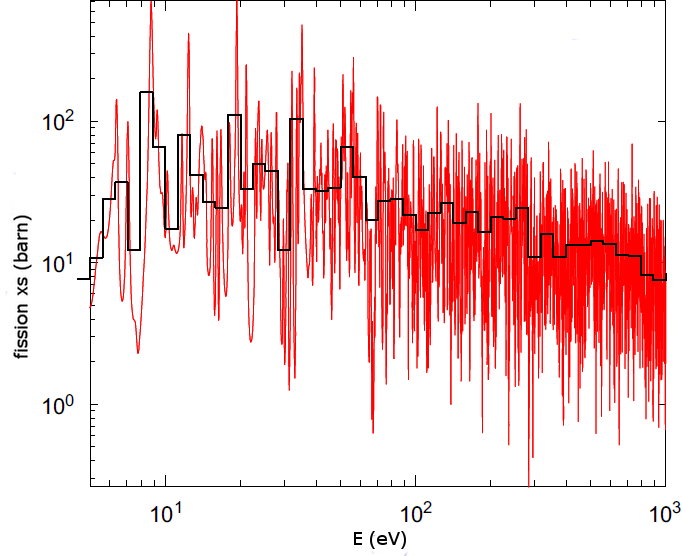
\includegraphics[scale=.4]{U235fg}
  \caption{Microscopic fission cross-section of U235}
  \label{fig:xs}
\end{center}
\end{figure}
Suitable approximation of the unknown exact solution in \eqref{eq:mg-kappa} is also highly non-trivial, albeit essential
for the success of the multigroup method. Even though an alternative to the finite-volume like approximation
\eqref{eq:psi-MG} has been proposed recently  in \cite{Douglass} -- using Galerkin projection of angular flux onto a
space of functions supported over subregions of the energy range (a finite-element like approach) --  the multigroup approximation still remains the most universally used approach to simplify the energetic dependence (see, e.g., \cite[Chap.~5]{Cacuci1} or \cite{Cho1}). However, we will
not specifically address this issue and always assume that the multigroup coefficients appearing in the equations 
are given as input.
\begin{remark}{\textsc{Fission spectrum}}
In criticality problems, the set of multigroup data must include both parts of the collision kernel
$\kappa^{gg'}$, i.e. the cross-sections $\sigma_s^{gg'}$ and $\sigma_f^{gg'}$, as well as $\nu^{g'}$ and
$\chi^g$ (neutron yield from inelastic scattering, $\eta$, is usually absorbed into $\sigma_s$). Because of the rapid
decay of $\chi(E)$ for low energies (as neutrons are mostly emitted with high energies from fission) that are
nevertheless the most important for the cross-sections (as most interactions are likely to occur due to slowly moving
neutrons, at least in classical moderated reactors)\footnote{cf. \fref{fig:xs} and \fref{fig:spectrum} and notice the
different scaling on the horizontal axis}, there will typically be $\chi^g = 0$ for $g = G,G-1,\ldots,G-k$. The
group-discretized operator $F$ from \eqref{eq:FScrit} will therefore have a non-trivial null-space, leading ultimately
to a fully discrete generalized eigenproblem of type $\mat{A}\mat{x} = \lambda\mat{B}\mat{x}$ with singular $\mat{B}$.
\end{remark}

A standard way of iterative solution of the multigroup system is the \textit{source iteration}:
\begin{equation}\label{eq:MGGS}
	\left(A + \Sigma_r^g\right)\psi^g_{(i+1)} = \summ{g'\leq g-1}{} K^{gg'}\psi^{g'}_{(i+1)} + \summ{g' \geq g+1}{}
  K^{gg'}\psi^{g'}_{(i)} + q^g,\quad g = 1,\ldots,G,\ \ i = 0,1,\ldots
\end{equation}
  This is a Gauss-Seidel iteration for the operator equation \eqref{eq:mg}, where the matrix operator $T_G$ has been
split into its lower-triangular part $A + \Sigma_r^g - K^{gg'}$ ($g'\leq g$) and its upper triangular part $K^{gg'}$
($g'> g$) and the lower triangular part is being inverted by forward substitution.
Note that a mono-energetic transport problem in group $g$ has to be solved in each iteration, and if neutron advection
can be approximated by a symmetric operator $\tilde A$, the problem would become symmetric with implications for
efficient numerical solution (see sections \ref{sec:second-order} and \ref{sec:algebraic} below). Convergence of this 
scheme can become slow when the upper triangular part (representing neutron up-scattering from lower energies to 
higher energies) is dominating. Therefore, when preparing the multigroup data, it may be advantageous to put an effort
into finding such an energy grouping that minimizes the up-scattering.
\begin{remark}\label{rem:SI}
Here we assume that the
mono-energetic problem can be solved exactly. Some transport approximations (like the $\SN$ method presented in
\sref{sec:1-SN}) typically employ another iteration level to resolve angular coupling of the within-group fluxes
induced by scattering. This iteration can also become very slow if scattering of
neutrons with given energy dominates their absorption and some acceleration is usually needed (we will return to this
issue later in \sref{sec:SI}).
\end{remark}

In the remainder
of this chapter, we will focus on the approximation of neutron flux in a single
group (index of which will be omitted), described by the corresponding within-group equation in which contributions from
other groups are encapsulated in the source term $\src$.

\section{Approximation of angular dependence}

A big number of methods have been proposed for approximating the angular dependence of neutron
flux. Many of them are still used and actively developed today as their characteristics make them more suitable for one
application area than other methods, which are preferred in different areas.

\subsection{Lattice calculations} \label{sec:lattice}
As a first example, we consider the class of
methods originally derived from the equivalent integral form of the NTE (see \sref{sec:advection}). Typical
representatives of this class are the method of collision probabilities or the method of characteristics (see e.g.
\cite{Cho2,Wu1,Hursin1,Petkov1,Sanchez1}). As the integral form of the NTE represents the global neutron balance over
the domain, the corresponding algebraic systems (obtained after spatial discretization) are full and
their solution demanding on computer resources. On the other hand, these methods quite naturally handle complex
geometries. Taking into consideration smaller geometric features of the domain, we are effectively coming from a
macroscopic scale to a mesoscopic range where the neutrons direction of motion as well as their kinetic energy become
more significant. High degree of spatial coupling and the requirement of fine resolution of angular and energetic
dependence does not make these methods suitable for whole-core reactor calculations.
However, these small-scale,
high-fidelity calculations\footnote{called \textit{lattice calculations} as they are typically performed on a single
representative subdomain of the core (one or several neighboring assemblies of fuel pins, or the fuel pin itself)
with reflective boundary conditions, simulating an infinite lattice of such subdomains} are indispensable for
generating appropriately averaged coefficients for the computationally more feasible larger scale calculations.
This \textit{spatial homogenization} and \textit{energy group condensation} (already mentioned in the previous
section), as these averaging procedures are traditionally called in nuclear engineering field, are employed by many existing whole-core simulators (see e.g.
\cite[Chap. 17]{Reuss1} or the review in first two sections of \cite{Sanchez7}). To simulate a long-term nuclear reactor
operation, it is furthermore neccessary to perform these procedures under varying physical conditions of the core and
generate many sets of averaged coefficients corresponding to these conditions. The code system described in
\cref{chap:coupled} expects these coefficient sets on input, i.e., it is not designed for lattice calculations.

\vspace*{1em}
More suitable for whole-core calculations are methods derived from the integro-differential
version of the NTE, eq.
\eqref{eq1}, which lead to sparse algebraic systems. The most successful and well-established are the method
of discrete ordinates ($\SN$) and the method of spherical harmonics ($\PN$).
Both arise from applying in the
angular domain a classical well known approach for constructing finite numerical
approximations of PDEs. \comment{Although in the final code, we ultimately use the lowest order approximation that can
be obtained equivalently from both approaches (the neutron diffusion model) we will briefly introduce the main ideas behind the
$\SN$ and $\PN$ methods and expose their most important properties in the next two subsections.} These properties are
generally known, but their origin in mathematical structure of the equations is mostly overlooked in
literature (rare exceptions will be cited below and in the corresponding appendices). 

\subsection{The $\SN$ method}\label{sec:1-SN}
The basic $\SN$ method uses the collocation approach in which a set of directions (\textit{ordinates})
$\omega = \{\bomega_n\}_{n=1}^{M}$ is chosen and the solution is approximated as:
\begin{equation}\label{eq:sn_approx} 
	\psi(\br, \bomega) \approx 
		\pw{\psi(\br,\bomega_n)}{if $\bomega = \bomega_n$ for $\bomega_n \in \omega$}
		   {0}{if $\bomega \not \in \omega$.} 
\end{equation}
Equation \eqref{eq1} as well as the boundary conditions \eqref{eq:nte2} or \eqref{eq:nte3} are then evaluated at these
$M = M(N)$ isolated directions. Notice that reflective (or albedo) boundary conditions place restrictions on the set of
ordinates as it should optimally contain both directions of each reflected pair (otherwise an interpolation would be
needed). For the traditional direction sets, we have $M = N(N+2)$ if the given problem does not possess any symmetries;
the method of discrete ordinates using such a number of directions is traditionally refered to as the method of 
discrete ordinates of order $N$, shortly $\SN$.

To evaluate the integral term on the right hand side of the equation, the set of directions is accompanied by a
corresponding set of weights $\{w_n\}_{n=1}^{M}$, together defining a quadrature of the sphere $\Sphere$. The
requirement of accurate evaluation of the integral term of eq.
\eqref{eq1} as well as accurate integration of the angular flux function over the sphere (to obtain the scalar flux)
constitutes the main guideline for the choice of directions and weights. We will return to this matter later in 
\sref{sec:DO}; for now it suffices to say that for three-dimensional problems without any symmetries, \mbox{$M = \left|\{\bomega_n, w_n\}\right| = \Oh(N^2)$} (with the
value of $M$ for typically used quadrature sets stated above).

To write  the final result of the $\SN$ approximation, let us first denote for a set $s = \{c_k\}_{k=1}^n$ the column
vector with entries $c_1,c_2,\ldots,c_n$ as $\col s$ and similarly the diagonal matrix whose diagonal is
given by elements of $s$ as $\diag(s)$. Then, denoting
\begin{equation}\label{eq:sn_vecs}
\psi_n(\br) \equiv \psi(\br,\bomega_n), \quad q_n(\br) \equiv
q(\br,\bomega_n),\quad n = 1,\ldots, M	
\end{equation}
we will define the vector of angular fluxes and the vector of angular sources as
\begin{equation}\label{eq:sn_vars}
\Psi(\br) := \col\{\psi_n(\br)\}_{\idxset{M}},\quad
\mat{Q}_{S_N}(\br) := \col\{q_n(\br)\}_{\idxset{M}},
\end{equation}
where we used the index set of $\SN$ variables: $\idxset{M} = \{1,2,\ldots,M\}$.
The $\SN$ approximation consists of the following set of $M$ PDEs in spatial domain\footnote{Differentiation and
integration of vector functions (such as the term $\pd{\Psi(\br)}{x}$ in eq. \eqref{eq:sn1}) is conventionally
understood component-wise.}:
\begin{equation}\label{eq:sn1} 
\mat{A}_{S_N}^x\pd{\Psi(\br)}{x} + \mat{A}_{S_N}^y\pd{\Psi(\br)}{y} +
\mat{A}_{S_N}^z\pd{\Psi(\br)}{z} + \bigl[\sigma_t(\br)\mat{I} - \mat{K}_{S_N}(\br)\bigr]\Psi(\br) = \mat{Q}_{S_N}(\br),
\end{equation}
where $\mat{I}$ is the $M\times M$ identity matrix,
$$
	\mat{A}_{S_N}^x = \diag\{\Omega_{n,x}\}_{\idxset{M}},\ \mat{A}_{S_N}^y = \diag\{\Omega_{n,y}\}_{\idxset{M}},\
	\mat{A}_{S_N}^z = \diag\{\Omega_{n,z}\}_{\idxset{M}}
$$
and
\begin{equation}\label{eq:SNK}
	\left[\mat{K}_{S_N}\right]_{m,n} = w_n \kappa(\bomega_m\cdot\bomega_n),\quad
	\bomega_n,\bomega_m\in \omega,\ w_n\in \mathcal{W},\ 1 \leq m,n \leq M.
\end{equation}


\subsubsection{Operator form}\label{sec:opsn}
In order to exhibit differences between the $\SN$ approximation and the $\PN$ approximation presented in the following
section, we write both methods as projections onto an appropriate approximation subspace. As motivated in
\cref{chap:nte-review}, we would like to continue with approximating generalized solutions of the NTE, for which the
classical view of the $\SN$ approximation relying on extracting pointwise values on the sphere is not appropriate. We
overcome this problem by formulating the $\SN$ method using a finite-volume need to specify a in the pre We will see
that the $\SN$ approximation space is quite poor and solutions found in this subspace by solving the $\SN$ system do not possess important properties of the true solution of the NTE, like the rotational invariance.

First, note that the $\SN$ approximation concerns only the angular variable. To reduce clutter, we will therefore drop
the spatial variable in the following discussion.
Consider now an arbitrary $\SN$ approximation specified by the given set of ordinates
$\omega = \{\bomega_n\}_{\idxset{M}}$ and a corresponding set of quadrature weights $\mathcal{W} =
\{w_n\}_{\idxset{M}}$.
%by using the Dirac measure $\delta_{\bomega}(\bomega')$ with the property
%\begin{equation}\label{eq:dirac}
%	\int_{\Sphere} f(\bomega')\d{\delta_{\bomega}(\bomega')} = f(\bomega).
%\end{equation}
For a vector (of functions of spatial variable) $\mat{F} = \colset{f_n}{\idxset{M}}$, we define the mapping
\begin{equation}\label{eq:map_SN}
\begin{gathered}
\PiSN: \mat{F} \mapsto f\in V_{S_N},\\
\bigl(\PiSN \Psi\bigr)(\bomega) = 
\pw{\psi_n}{if $\bomega = \bomega_n$ for $\bomega_n \in \omega$}{0}{if $\bomega \not
	\in \omega$}
\end{gathered}
\end{equation}
$V$ is some general function space ensuring existence of unique solution of the NTE (see \sref{sec:fixed-source} for
examples) and $V_{S_N}\subset V$ is its subspace containing functions vanishing (as functions of $\bomega$) everywhere
on $\Sphere$ except at $\bomega \in \omega$. Note that this mapping converts a vector of directional fluxes to a 
function on $\Sphere$. Corresponding to it is the mapping that produces the discrete ordinates representation of a 
function $f$ defined on $\Sphere$:
\begin{equation}\label{eq:map_SN_inv}
	\PihSN f(\bomega) := \col\left\{f_n \right\}_{\idxset{M}}
	 = \col\left\{f(\bomega_n)\right\}_{\idxset{M}}
\end{equation}
(which we implicitely used in \eqref{eq:sn_vars} with $f(\cdot,\bomega) = \psi(\cdot,\bomega)$ and
$f(\cdot,\bomega) = q(\cdot,\bomega)$, respectively, and which also applies to functions representing the
inflow boundary conditions).
With these two mappings, we can rewrite the $\SN$ system \eqref{eq:sn1} in terms of the transport operators from eq.
\eqref{eq1op}:
\begin{equation}\label{eq:sn_op}
	\PihSN (\op{L} - \op{K}_{S_N}) \PiSN \Psi = \mat{Q}_{S_N},
\end{equation}
where $\op{K}_{S_N}: V_{S_N} \to V$ is the $\SN$ quadrature representation of the original integral operator
$K$, defined as follows: 
\begin{equation}\label{eq:KSN}
	\op{K}_{S_N} f(\bomega) = \sum_{n=1}^{M} w_n \kappa(\bomega\cdot\bomega_n) f(\bomega_n), \quad \bomega_n\in \omega,\ 
	w_n\in \mathcal{W}. 
\end{equation}
Note that the operator $\PihSN (\op{L} -
\op{K}_{S_N}) \PiSN$ maps $M$-vectors to $M$-vectors and represents the $\SN$ matrix. The
final $\SN$ approximation of the original transport operator is obtained as an operator $V \to V_{S_N}$ by incorporating the definition of the $\SN$ unknowns $\Psi$ from a function
$\psi \in V$ and representing the output again as a function. This leads to the following formulation:
\begin{equation}\label{eq:sn_op}
	\PiSN \PihSN (\op{L} - \op{K}_{S_N})\PiSN \PihSN \psi = \PiSN \PihSN q,
\end{equation}
or
\begin{equation}\label{eq:sn_op2}
	\Projop[S_N]  (\op{L} - \op{K}_{S_N}) \Projop[S_N] \psi = \Projop[S_N] q
\end{equation}
where
\begin{equation}\label{eq:proj_sn}
	\Projop[S_N] := \PiSN \PihSN, \quad \Projop[S_N] : V \to V_{S_N}.
\end{equation} 
It is clear from the definitions \eqref{eq:map_SN} and \eqref{eq:map_SN_inv} that when restricted to $V_{S_N}$, 
\linebreak[3]\mbox{$\PihSN = \PiSN^{-1}$} and hence $\Projop[S_N]^2 = Id$, where $Id : V_{S_N} \to V_{S_N}$ is the
identity operator on $V_{S_N}$.
 Therefore, $\Projop[S_N]$ represents a projection onto the $S_N$ approximation space (and formalizes eq.
 \eqref{eq:sn_approx}).


\subsubsection{Structure of the $\SN$ approximation}
Equation \eqref{eq:sn1} represents a system of advection-reaction equations, each with constant advection field given by
the matrices $\mat{A}_{S_N}^x, \mat{A}_{S_N}^y, \mat{A}_{S_N}^z$.

Let us for a moment consider the steady-state $\SN$ equations as a limit of the 
time-dependent equations
\begin{equation}\label{eq:PN_ss_app}
	\PihSN \left(\pd{}{t} + A + C\right) \PiSN\Phi = \PihPN q,
\end{equation}
in which $\pd{}{t}\PiSN\Phi \to 0$, for time-independent boundary conditions and sources
\linebreak[3]\mbox{$q(\cdot,\cdot,t) = \text{const}$}.
Then, the advection matrices describe advection of neutrons introduced into the system by the boundary and internal
sources, which is in the steady-state limit perfectly balanced by their capture.

As we can see from \eqref{eq:KSN}, the term $\mat{K}_{S_N}\Psi$ induces full unknown coupling. In order to recover 
sparsity (and also facilitate the use of efficient constant-advection solvers based on explicit marching in the advection direction), the so-called  \textit{scattering
source iteration} is utilized, in which the system \eqref{eq:sn1} is fully decoupled by moving $\mat{K}_{S_N}$ to the
right. Each equation is solved separately using any method suitable for an advection-reaction PDE with constant
advection vector, using $\psi_n$ from previous iteration to evaluate $\mat{K}_{S_N}\Psi$. Classical iteration methods
like Jacobi and Gauss-Seidel are typically used to update $\Psi$ during the iteration process; e.g. the Jacobi scheme 
gives the iteration
\begin{equation}\label{eq:SI}
	\mat{A}_{S_N}^x\pd{\Psi_{(i+1)}}{x} + \mat{A}_{S_N}^y\pd{\Psi_{(i+1)}}{y} +
	\mat{A}_{S_N}^z\pd{\Psi_{(i+1)}}{z} + \sigma_t\mat{I}\Psi_{(i+1)}= \mat{K}_{S_N}\Psi_{(i)} +
	\mat{Q}_{S_N},\quad
	i = 0,1,\ldots
\end{equation}
for given initial approximation $\Psi_{(0)}$. We will return to the convergence characteristics of this iteration later;
for now, assume that a converged solution vector $\Psi = \colset{\psi_n}{M}$ has been obtained. The important physical
quantities (scalar flux, neutron current) are then obtained directly from their definition \eqref{eq:scalar_flux} and \eqref{eq:bJ} using
the quadrature formula, e.g.
$$
	\phi(\br) = \intA{\psi(\br,\bomega)} = \sum_{n=1}^{M} w_n \psi(\br,\bomega_n) = \sum_{n=1}^{M} w_n \psi_n, \quad \br\in
	\VV,\ \bomega_n\in \omega,\ w_n\in \mathcal{W}.
$$

\myparagraph{Ray effects}
A major drawback of the $\SN$ angular approximation comes from the fact that it propagates radiation 
only in a discrete set of directions. Only in the limiting case of infinite number of directions will the
whole phase space be covered. Otherwise, there will remain under-treated regions, while other regions will receive more radiation in order
to satisfy the global balance. This will lead to spatial oscillations of the scalar flux  known as the \textit{ray
effects}. The root cause of ray effects is often attributed to the intuitively obvious lack of rotational invariance 
(\cite{Reuss}, \cite{Sanchez6}), which shows that the important property of the NTE is not carried over to the $\SN$
approximation. Various remediesWe give now a rigorous proof of this fact for the simplified transport problem without
scattering, using the operator form of the $\SN$ equations developed in the previous subsection. We remark that scattering can somewhat ameliorate the
 oscillations caused by ray effects as it increases the coupling between directional fluxes, but it cannot remove the
 inherent lack of rotational invariance of the $\SN$ approximation.




\label{sec:SI}
\comment{
Writing the iteration in the form
$$
\PihSN \op{L} \PiSN  \Psi_{(i+1)} = \PihSN \op{K}_{S_N} \PiSN \Psi_{(i)} + \mat{Q}_{S_N},
$$
we can see that propert It can be shown by Fourier analysis that
in an infinite homogeneous medium, the iteration \eqref{eq:SI} suppresses those Fourier modes with wavelengths  see also Remark \ref{rem:SI}).
\cite[Chap. 1]{Azmy1}, or \cite[Sec. II.A]{Adams})
}



 
\begin{theorem*}\label{thm:commut_NTE}
Let $L : V\to V$ be the advection-collision operator of the NTE satisfying
$RL = LR$ for all $R\in\mathrm{SO}(3)$. 
Then the corresponding $\SN$ approximation operator
\begin{equation}\label{eq:sn_op_app}
	\Projop[S_N]\op{L}\Projop[S_N]
\end{equation}
(with $\Projop[S_N]$ defined by \eqref{eq:proj_sn}, \eqref{eq:map_SN}, \eqref{eq:map_SN_inv} and particular
ordinates and quadrature sets \mbox{$\omega = \{\bomega_n\}_{\idxset{M}}$, $\mathcal{W} = \{w_n\}_{\idxset{M}}$})
satisfies $$
\op{R}\op{L}\Projop[S_N] = \op{L}\Projop[S_N]\op{R}\quad \forall R\in\mathrm{SO}(3)
$$
if and only if
\begin{equation}\label{eq:thm1_cond}
	\forall n\in \idxset{M}\ \exists m\in\idxset{M}: \mat{R}\bomega_n = \bomega_m \quad \forall \mat{R}\in\mathrm{SO}(3).
\end{equation} 
\end{theorem*}
\begin{remark*}
	Note that the conditions \eqref{eq:thm1_cond} can be satisfied only in the limit \mbox{$M\to\infty$}.
\end{remark*}
\begin{proof}
First, recall from \sref{sec:opsn} that for any $\SN$ approximate function \mbox{$f_{S_N}\in V_{S_N}$}, 
$$
	\Projop[SN]f_{S_N} = f_{S_N}.
$$
Also, for $\psi_{S_N} \in V_{S_N}$:
$$
	\bomega\cdot\nabla\psi_{S_N}(\br,\bomega) = \left.\pw{
		\bomega_n\cdot\nabla\psi(\br,\bomega_n)}{if $\bomega = \bomega_n$ for $\bomega_n\in\omega$}
		{0}{if $\bomega \not \in \omega$.}\right\} \in V_{S_N}
$$
where we recall the characterization of $V_{S_N}$ as a space of functions that, as functions of $\bomega$, vanish
everywhere on $\Sphere$ except points corresponding to the selected ordinates set. Therefore for $\psi_{S_N} \in
V_{S_N}$, 
$$
	L\psi_{S_N} \equiv \bomega\cdot\nabla\psi_{S_N} + \sigma_t\psi_{S_N} \in V_{S_N}.
$$
Since \mbox{$\Rng (\PiSN) = V_{S_N}$}, it follows that the $\SN$ operator \eqref{eq:sn_op_app} can be simplified as:
\begin{equation}\label{eq:sn_op2}
	\Projop[S_N]\op{L}\Projop[S_N] = \op{L} \Projop[SN].
\end{equation}
Because of the commutativity of $L$ and $R$, it therefore suffices to show that $\Projop[S_N]$ commutes
with $\op{R}$, that is (using def. \eqref{eq:proj_sn})
\begin{equation}\label{eq:thm1_point}
	R \PiSN \PihSN \psi = \PiSN \PihSN R \psi\quad  \forall \psi \in V, 
\end{equation}
if and only if the condition \eqref{eq:thm1_cond} holds.\\[.2em] 

As in \sref{sec:opsn}, we will suppress the spatial dependence as the $\SN$ approximation concerns only the angular
dependence. For any $\psi\in V$, we have
\begin{equation*}
	\PihSN R\psi(\bomega) = \colset{R\psi(\bomega_n)}{\idxset{M}} = \colset{\psi(\mat{R}^T\bomega_n)}{\idxset{M}}.
\end{equation*}
Applying $\PiSN$ thus yields a function $f_\psi = \PiSN\PihSN R\psi \in V_{S_N}$ such that
\begin{equation}\label{eq:thm1_f}
f_\psi(\bomega) = \pw{\psi(\mat{R}^T\bomega_n)}{if $\bomega = \bomega_n$ for $\bomega_n\in\omega$}{0}{if $\bomega \not
	\in \omega$.}
\end{equation}
On the other hand, let $u = \PiSN\PihSN\psi$. Then
$$
u(\bomega) = \pw{\psi(\bomega_n)}{if $\bomega = \bomega_n$ for $\bomega_n\in\omega$}{0}{if $\bomega \not
	\in \omega$}
$$ 
and the rotated function $g_\psi(\bomega) = R\PiSN\PihSN\psi = R u(\bomega)$ is given by
$$
g_\psi(\bomega) = u(\mat{R}^T\bomega) = \pw{\psi(\bomega_n)}{if $\mat{R}^T\bomega = \bomega_n$ for
$\bomega_n\in\omega$}{0}{if $\mat{R}^T\bomega \not \in \omega$}
$$
or, equivalently, by
\begin{equation}\label{eq:thm1_g}
g_\psi(\bomega) = \pw{\psi(\bomega_n)}{if $\bomega = \mat{R}\bomega_n$ for
$\bomega_n\in\omega$}{0}{if $\bomega \not \in \mat{R}\omega$}
\end{equation}
(where action of $\mat{R}$ on the set $\omega$ is understood element-wise). If the ordinate set $\omega$ contains for
any ordinate $\bomega_n$ also its rotated copy $\mat{R}\bomega_n$, i.e., condition \eqref{eq:thm1_cond} holds, then also
$$
	\bomega_n = \mat{R}^T\bomega_m
$$
and after simple substitution in \eqref{eq:thm1_g} and renumbering in \eqref{eq:thm1_f}, we obtain
$$
	f_\psi(\bomega) = g_\psi(\bomega).
$$
In order for this equality to hold true for any $\psi \in V$ (and hence for \eqref{eq:thm1_point} to hold true), the
condition \eqref{eq:thm1_f} is also necessary.
\end{proof}


\subsection{The $\PN$ method}\label{sec:PN}

Instead of the collocation method used by the $\SN$ approximation, the $\PN$ method uses the Galerkin weighted residuals
approach in the angular domain. That is, the angularly dependent quantities in \eqref{eq1} are expanded into infinite
series of properly chosen functions that span a complete basis on the unit sphere, the equation is multiplied by each member of the basis in turn
and integrated over the sphere. The properties of the basis functions are then used to derive equations for
the expansion coefficients. Only a finite number of the expansion terms is considered to allow practical computation.
Usually, the expansion is truncated to a finite length of $K = K(N)$ terms\footnote{The length of the expansion $K$
should not be confused with the operator $K$ introduced in the previous section; it will be always clear from context 
which meaning the letter $K$ currently has.} by setting all expansion coefficients with higher index to 0 (although there exist alternative closure methods that may have favorable properties in certain situations, see e.g.
\cite{Frank0}). Then we speak of the $\PN$ approximation:
\begin{equation}\label{eq1.1}
  \psi(\br,\bomega) \approx \sum_{k=1}^{ K} \phi_k(\br) f_k(\bomega).
\end{equation}
A natural function space to support this procedure is the Hilbert space of 
square-integrable functions on the sphere $\Lp[2](\Sphere)$, equipped with the inner product
\begin{equation}\label{eq:s2_ip}
	(u, v)_{\Lp[2](\Sphere)} = \intA{u(\bomega) {v(\bomega)}}.
\end{equation}
We will therefore assume \mbox{$\psi(\cdot,\bomega)\in\Lp[2](\Sphere)$} in this section. 

The system of spherical basis functions that were used in the original $\PN$ method are the
\textit{spherical harmonic functions} (shortly \textit{spherical harmonics}, App. \ref{app:SH}). We will consider
here the real system (whose elements are sometimes called \textit{tesseral spherical harmoncs}) as it is more convenient
for practical purposes than the equivalent complex system (which appears to be more traditional in nuclear engineering 
literature, e.g. \cite[Sec. 9.7]{Stacey}, \cite[Sec. 14.4]{Reuss}), \cite[Chap. V]{Stammler}). Spherical harmonics form
a complete orthonormal system on $\Lp[2](\Sphere)$ with respect to the inner product \eqref{eq:s2_ip} (or its Hermitian 
variant when complex spherical harmonics are used) and simplify the algebraic manipulations needed to arrive at the 
conditions for coefficients $\phi_k$ (called \textit{angular moments}). In one dimension, spherical harmonics reduce to 
Legendre polynomials and $ K(N) = N$.
For general three-dimensional problems, there are $2n + 1$ linearly independent spherical harmonics for each degree $n$ 
and 
$$ 
	K(N) = \sum_{n=0}^{N} 2n + 1 = (N+1)^2.
$$

The approximation \eqref{eq1.1} is usually rewritten as
\begin{equation}\label{eq:pn_approx}
	\psi(\br,\bomega) \approx \sum_{k=1}^{ K} \phi_k(\br)\Y{k}{}(\bomega) \equiv
	\suma[n]{0}{N}\suma[m]{-n}{n}\angmom{n}{m}(\br)\Y{n}{m}(\bomega)
\end{equation}
where $\Y{n}{m}(\bomega)$ is the spherical harmonic function of degree $n$ and order $m$
and in the first term on right, we consider the single index $k$ ($1 \leq k \leq  K$) that covers all the combinations of $n$ and $m$ ($0 \leq n \leq N$, $-n\leq m \leq n$) appearing in the second term. We finally arrive at a system of $ K$
partial differential equations in spatial domain which is of comparable size as the system of $\SN$ equations and has the following form:
\begin{equation}\label{eq:pn1}
	\mat{A}^x_{P_N}\,\pd{\Phi(\br)}{x} + \mat{A}^y_{P_N}\,\pd{\Phi(\br)}{y} + \mat{A}^z_{P_N}\,\pd{\Phi(\br)}{z} +
	\bigl[\sigma_t(\br)\mat{I} - \mat{K}_{P_N}(\br)\bigr]\Phi(\br) = \mat{Q}_{P_N}(\br),
\end{equation}
where 
\begin{equation}\label{eq:pn_vectors}
	\Phi = \col\left\{\phi_k\right\}_{\idxset{K}} \ \text{ and }\ 
	\mat{Q}_{P_N} = \col\left\{q_k\right\}_{\idxset{K}}
\end{equation}
are, respectively, the vector of angular flux
moments and angular source moments, and the index set of $\PN$ variables is defined analogously to the $\SN$ case:
$$
\idxset{K} = \{1,2,\ldots,K\}.
$$
The
Galerkin procedure results in their special form
\begin{equation}\label{eq:pn_angmom}
	\phi_k = (\psi, \Y{k}{})_{\Lp[2](\Sphere)},\quad q_k = (q, \Y{k}{})_{\Lp[2](\Sphere)}
\end{equation}
which, in view of \eqref{eq:pn_approx} and the completeness and orthogonality properties of spherical harmonics, also 
shows that the angular flux in the $\PN$ method is actually approximated by its orthogonal projection onto the
finite-dimensional subspace $\Lp[2]_K(\Sphere)\subset\Lp[2](\Sphere)$:
\begin{equation}\label{eq:PN_proj}
	\Projop\psi(\cdot,\bomega) := \sum_{k=1}^{ K}\ips{\psi}{\Y{k}{}} \Y{k}{}(\bomega).
\end{equation}
We also have a direct correspondence of the first four moments and the physically important quantities defined in
\sref{sec:qoi}:
$$
	\phi = \sqrt{4\pi}\angmom{0}{0},\quad \bJ = \sqrt{\frac{4\pi }{3}}\, [\angmom{1}{1}, \angmom{1}{-1}, \angmom{1}{0}]^T.
$$

\subsubsection{Operator form} \label{sec:pn_op}
As in the $\SN$ case, the $\PN$ system \eqref{eq:pn1} can be put into a form involving the transport operators from eq.
\eqref{eq1op}.
In order to do so, let us define mappings that take the vector $\Phi(\cdot)$ of angular flux moments to angular
flux $\psi(\cdot,\bomega)\in\Lp[2]_K(\Sphere)$ and vice versa. The general operators realizing this operation for the
case $\mat{F} = \Psi$ and $f(\bomega) = \psi(\cdot,\bomega)$, respectively, are
\begin{equation}\label{eq:pn_op_def}
\bigl(\PiPN\mat{F}\bigr)(\bomega) := \sum_{k=1}^{ K} f_k\Y{k}{}(\bomega), \quad
\PihPN f(\bomega) = \col \left\{(f, \Y{k}{})_{\Lp[2](\Sphere)}\right\}_{\idxset{K}}.
\end{equation} 
Using \eqref{eq:pn_angmom}, \eqref{eq:pn_vectors} and \eqref{eq:PN_proj}, we can see that 
$$
\PiPN\Phi = \PiPN\PihPN \psi = \Projop\psi.\footnote{Again as in the $\SN$ case, when restricted to the space of functions that (as functions of $\bomega$) can be
expressed as linear combination of spherical harmonics up to degree $N$, $\PihPN = \PiPN^{-1}$ (which is equivalent to $\Projop[P_N]$ being
a projection).}
$$ 
The operator form of the $\PN$ system is thus
\begin{equation}\label{eq:pn_op}
	\PihPN (L-K) \PiPN\Phi = \mat{Q}_{P_N} = \PihPN q
\end{equation}
or
\begin{equation}\label{eq:pn_op2}
	\Projop (L-K) \Projop\psi = \Projop q.
\end{equation}

\subsubsection{Structure of the $\PN$ system}
\myparagraph{Advection part}
The system has the same form as that for the $\SN$ approximation, but the advection matrices:
\begin{equation}\label{eq:advmat_PN}
	\left[\mat{A}_{P_N}^s\right]_{k,l} = \intA{\Omega_s \Y{k}{}(\bomega)\Yc{l}{}(\bomega)},\quad s\in\{x,y,z\},\ 
	1 \leq k,l \leq  K
\end{equation}
are no longer diagonal (although they couple no more than 6 angular flux moments, see \ref{app:C} for an example for $N
= 3$ or \cite[App. A]{Sanchez8} for general treatment). Each of the advection matrices \eqref{eq:advmat_PN} 
is symmetric and hence for any $\bn = [n_x,n_y,n_z]^T$, 
$$
	\mat{A}_{P_N}^{\bn} = n_x \mat{A}_{P_N}^x + n_y \mat{A}_{P_N}^y + n_z \mat{A}_{P_N}^z
$$
is symmetric and diagonalizable with real eigenvalues. The $\PN$ system is thus (strongly) hyperbolic in the sense of 
\cite[Def. 18.1]{leveque}. The eigenvalues depend on 
$\bn$ only through its length $\norm{\bn}$ (see \sref{app:C} for an example when $N = 3$,  though this property
holds for general $N$), which shows that the $\PN$ system propagates radiation at the same speed in any
direction. This is in a contrast to the $\SN$ advection \footnote{Here we consider the $\PN$ system as a steady-state
limit of the time-dependent equation, as explained in \sref{app:C}.}.

It is more convenient for this analysis to consider the steady-state $\PN$ equations \eqref{eq:PN_ss_app} as a limit of the 
time-dependent equations
\begin{equation}\label{eq:PN_ss_app}
	\PihPN \left(\pd{}{t} + A + C\right) \PiPN\Phi = \PihPN q,
\end{equation}
in which $\pd{\psi}{t} \to 0$, for time-independent boundary conditions and sources
\linebreak[4]\mbox{$q(\cdot,\cdot,t) = \text{const}$}.
Then, the advection matrices describe advection of neutrons introduced into the system by the boundary and internal
sources, which is in the steady-state limit perfectly balanced by their capture.

This hints that rotational invariance of the NTE is preserved by the $\PN$ system, as we will directly show in 
\sref{sec:dirinvPN}. The eigenstructure of the advection matrices also provides a clue on how many boundary conditions
should be prescribed for the $\PN$ system. Matrix $A_{P_N}^{\bn}$ for given $N$ has
$N(N+1)/2$ positive eigenvalues, $N(N+1)/2$ negative eigenvalues and $K(N) - N(N+1) = N+1$ zero eigenvalues,
irrespective of $\bn$. If we take $\bn$ to be the unit outward normal to $\pV$, these eigenvalues correspond,
respectively, to outgoing, incoming and tangential neutron radiation waves. In order for the hyperbolic system to be
well-posed, we are allowed to prescribe only the incoming waves, hence we are allowed to specify $N(N+1)/2$ boundary
conditions at any point of the boundary. It is more difficult to determine what the conditions actually look like as the
waves generally contain components of all moments $\angmom{n}{m}$. On the grounds of physical reasoning
(e.g. \cite{Rumyantsev}), variational analysis (e.g. \cite{Davis}) or most recently the equivalence between hyperbolic
and elliptic forms of the $\PN$ equations (\cite{Sanchez8}), the agreed upon form of $\PN$ boundary conditions
consistent with the present Galerkin framework is obtained (e.g. for the incoming condition \eqref{eq:nte2}) as:
$$
\begin{gathered}
	\left(\psi_\text{in} - \left.\Projop[P_N]\!\psi\right\vert_{\pX[-]}, \Y{p}{m} \right)_{\Lp[2](\pX[-])} = 0,\\[.35em] 
	p = 
	\left.\begin{cases}
		0,2,4,\ldots,N\!-\!1 & \mbox{ for $N$ odd}\\
		1,3,5,\ldots,N\!-\!1 & \mbox{ for $N$ even}	
	\end{cases}\right\},\ -p \leq m \leq p;
\end{gathered}
$$
that is, as (oblique) projection of the specified incoming angular flux onto $\Lp[2]_N(\pX[-])$, orthogonal
to the subspace of $\Lp[2](\pX[-])$ spanned by spherical harmonics with even/odd degrees, with respect to the inner product
$$
	\left(u,v\right)_{\Lp[2](\pX[-])} = \int_{\pV}\int_{\bomega\cdot\bn < 0}\abs{\bomega\cdot\bn}
	u(\br,\bomega)v(\br,\bomega)\,\d{\br}\d{\bomega}.
$$
We will call boundary conditions of this form (as in \cite{Davis}) \textit{Marshak boundary conditions}.

\myparagraph{Collision part}
As we have discussed above, the increased coupling between the
unknowns in the $\PN$ system may be seen as a price for rotational invariance
that prevents ray effects appearing in $\SN$ solutions. On the other hand, the collision matrix $\mat{K}_{P_N}$ is
diagonal, which can make the method computationally more attractive than the fully coupled $\SN$ method in cases when 
scattering source iteration cannot be efficiently used. This property is a consequence of the following lemma:

\begin{lemma}\label{lem:appC}
The spherical harmonic functions $\Y{n}{m}$ diagonalize the collision operator $K$ and
$$
	K\Y{n}{m} = \kappa_n \Y{n}{m},\quad n = 0,1,\ldots,\quad -n \leq m \leq n,
$$
where
$$
	\kappa_n = 2\pi \muint[_0]{\P{n}{}(\mu_0)\kappa(\mu_0)},\quad \mu_0 = \bomega\cdot\bomega'
$$
is the $n$-th Legendre moment of the collision kernel $\kappa$.
\end{lemma}  
\begin{proof}
	As we assume the collision kernel to be a square integrable function of the collision cosine  
	$\mu_0 \equiv \cos \polar_0 = \bomega\cdot\bomega'$ (see \fref{fig:scatter})
	and the Legendre polynomials \eqref{eq:leg} form a complete orthogonal system on $\Lp[2]([-1,1])$, we can express the
	collision kernel as a sum of the Fourier series
	$$
		\kappa(\mu_0) = \suma[n]{0}{\infty}\frac{2n+1}{4\pi}\kappa_n\P{n}{}(\mu_0),\quad
		\kappa_n = 2\pi \muint[_0]{\kappa(\mu_0)\P{n}{}(\mu_0)}.
	$$
	Then for any $n = 0,1,\ldots,\quad -n \leq m \leq n$,
	$$
\begin{aligned}
	K\Y{n}{m}(\bomega) &= \intA[']{\kappa(\bomega\cdot\bomega')\Y{n}{m}(\bomega')} \\
	&= \intA[']{\suma[r]{0}{\infty}\frac{2r+1}{4\pi}\kappa_r\P{r}{}(\bomega\cdot\bomega')\Y{n}{m}(\bomega')} \\
	&= \suma[r]{0}{\infty}\kappa_r\suma[s]{-r}{r}\Y{r}{s}(\bomega)\intA[']{\Y{r}{s}(\bomega')\Y{n}{m}(\bomega')} \\
	&= \kappa_n\Y{n}{m}(\bomega).
\end{aligned}
	$$
	where the addition theorem \eqref{eq:additionThm} has been used on third line and orthogonality relation \eqref{eq:og}
	on the fourth, completing the proof.
\end{proof}

\begin{corollary}
	Matrix $\mat{K}_{P_N} = \PihPN K \PiPN$ is diagonal, with entries given by the (repeated) Legendre moments $\kappa_n$.
\end{corollary}
\begin{proof}
	The $j$-th column of $\mat{K}_{P_N}$ is given by
	$$
		\mat{K}_{P_N}\mat{e}_j = \PihPN K \PiPN \mat{e}_j,
	$$
	where $\mat{e}_j$ is the $j$-th canonical basis vector in $\R[K]$. By definition, each index \mbox{$j = 0,1,\ldots K$}
	corresponds to a unique double index ${}_n^m$ ($n = 0,1,\ldots N$, $-n \leq m \leq n$), so that $\Y{j}{} \equiv
	\Y{n}{m}$.
	We can therefore write 
	$$
		\bigl(\PiPN \mat{e}_j\bigr)(\bomega) = \Y{j}{}(\bomega) = Y_n^m(\bomega).
	$$
	Using lemma \ref{lem:appC}, we have 
	$$
		K \PiPN \mat{e}_j = \kappa_n \Y{n}{m}
	$$
	so, when associating the index $i$ to a double index ${}_r^s$ and using the orthogonality relation \eqref{eq:og},
	$$
	\left[\mat{K}_{P_N}\right]_{ij} = \left[\PihPN K \PiPN \mat{e}_j\right]_i = (\kappa_n \Y{n}{m},
		\Y{r}{s})_{\Lp[2](\Sphere)} = \kappa_n\delta_{n}^{r}\delta_{m}^{s} = \kappa_n\kron{i}{j}
	$$
	Note that there is a single value $\kappa_n$ for all $2n + 1$ functions  $\Y{n}{m}$, so the $\mat{K}_{P_N}$ consists of
	$N+1$ diagonal blocks having consecutively $\lambda_0$, 3 times $\lambda_1$, 5 times $\lambda_3$, etc.  as their
	entries.
\end{proof}
\begin{corollary}
The complete ``capture'' matrix 
$$
	\mat{C}_{P_N} = \PihPN C \PiPN \equiv \PihPN (\Sigma_t - K) \PiPN 
$$
(corresponding to the capture cross-section $\sigma_c$ in \eqref{eq:st} and characterizing net neutron loss due to
all types of neutron-nuclei interactions) is diagonal.
\end{corollary}
\vspace*{1em}
\begin{remark}[\textsc{Isotropic scattering moment}]\label{rem:app:c}
	Fix a direction $\bomega\in\Sphere$ (the outgoing direction). Then the $0$-th Legendre moment of the scattering
	component of the collision kernel $\kappa$ (i.e. the first term on the right of \eqref{eq:splitting}), satisfies 
	$$
		\sigma_{s0} = 2\pi \muint[_0]{\P{0}{}(\mu_0)\sigma_s(\mu_0)} = \int_{0}^{2\pi} \int_{0}^{\pi}
		\sigma_s(\cos \polar_0) \sin \polar_0\d{\polar_0} = 
		\int_{\Sphere} \sigma_s(\bomega\cdot\bomega') \d{\bomega'}.
	$$
	Comparing with def. \eqref{eq:ddifxs}), 
	$$
		\sigma_{s0} = \eta\sigma_s
	$$
	i.e., the $0$-th Legendre moment of scattering represents the expected number of neutrons coming out of 
	scattering collisions in any direction.
\end{remark} 

\subsubsection{Rotational invariance of the $\PN$ equations}\label{sec:dirinvPN}
The increased coupling between the unknowns in the $\PN$ system is the price for rotational invariance of spherical
harmonics that prevents ray effects appearing in $\SN$ solutions. To prove it, we will use some well known facts about
spherical harmonics (see e.g, \cite[Chap.
3]{Sansone}, \cite[Sec. 3.9]{Schreiner}). 

\comment{
\myparagraph{Orthogonal decomposition of $\Lp[2](\Sphere)$}
Spherical harmonic functions of given degree $n$ generate a rotationally invariant subspace
of $\Lp[2](\Sphere)$, which we denote by $\Lambda_n$:
\begin{equation}
	\label{eq:subspace}
    	\Lambda_n = \text{Span}\bigl\{\Y{n}{m}; -n \leq m \leq n\bigr\},
\end{equation}
This means that $\op{R}(\Lambda_n) \subset \Lambda_n$ for any rotation transformation $\op{R}\in\mathrm{SO}(3)$. 
Moreover, there is no proper subspace $\Lambda_n' \subset \Lambda_n$ that is rotationally invariant by itself. For given $n$, $\Lambda_n$ is the eigenspace associated with
the $n$-th eigenvalue of the Laplace operator on $\Sphere$:
$$
	\lap_{\Sphere} \Y{n}{m}(\bomega) = -n(n+1)\Y{n}{m}(\bomega) \quad \forall -n \leq m \leq n.
$$

Being finite-dimensional eigenspaces of a self-adjoint operator
corresponding to different eigenvalues, $\Lambda_n$ for $n=0,1,\ldots$ are mutually orthogonal, closed subspaces of
$\Lp[2](\Sphere)]$ and $\Lp[2](\Sphere) = \bigoplus_{n=0}^{\infty}\Lambda_n$\nomenclature[S]{$\bigoplus$}{direct sum of
spaces}.
Restricting to a finite direct sum, we can hence write the $\PN$ projection \eqref{eq:PN_proj} as
\begin{equation}\label{eq:pn_approx2}
	\Projop\psi(\cdot,\bomega) = \suma[n]{0}{N}\Projop[\Lambda_n]\psi(\cdot,\bomega),
\end{equation}
where 
$$
	\Projop[\Lambda_n]\psi(\br,\bomega) = \suma[m]{-n}{n}\angmom{n}{m}(\cdot)\Y{n}{m}(\bomega)
$$
is the orthogonal projection onto $\Lambda_n$.  
}


\subsubsection{Drawbacks of the $\PN$ approximation}
Using the results of the previous paragraph and well-known results from the theory of Hilbert spaces, we can see that
the sum \eqref{eq:pn_approx2} (or \eqref{eq:pn_approx}) converges in the $\Lp[2](\Sphere)$ norm to the true solution of
eq. \eqref{eq1} as $N\to\infty$. However, the convergence may be very slow if the true solution to the NTE is not
sufficiently regular in the angular variable. In particular, pointwise convergence is hindered in the neighborhood of
phase space points where the solution of the NTE has jump discontinuity in $\bomega$ (which may occur for example when a
narrow beam of neutrons is freely streaming through a non-interacting medium, but, as we already mentioned at the
beginning of \sref{sec:ntp}, also in a more typical case of domains with multiple regions with different materials,
bounded by piecewise polygonal boundary) and spurious oscillations are introduced to the approximate solution at these points.
These oscillations spread over the whole angular domain and slow down the norm-wise convergence. This is a well-known
property of Fourier series (which the expansion \eqref{eq:pn_approx2} generalize) known as \textit{Gibbs phenomenon}.
Moreover, these oscillations do not vanish as more terms in the series are retained. However, there are several ways of
circumventing the Gibbs phenomenon. For example, when considering \eqref{eq:pn_approx2} as a means of deriving the $\PN$
system, we may note that using a finite expansion obtained by truncating \eqref{eq:pn_approx2} at $n=N$ is not the only
way of obtaining a closed system of equations -- different closures are possible as already discussed above. This fact
has been utilized in \cite{McClarren3} where the expansion has been adjusted to mitigate the oscillations by controlling
angular gradients\footnote{Note that the expansion \eqref{eq:pn_approx2} represents the best $\Lp[2](\Sphere)$
approximation of $\psi$ by spherical polynomials up to a given degree, but absence of angular gradients in the
$\Lp[2](\Sphere)$ norm permits arbitrary oscillations.}. For other similar approaches in the context of general spectral
methods, see e.g. \cite{Tanner}.

As shown in \cite{McClarren4}, there is also another issue connected with time-dependent $\PN$ approximation that must
be kept in mind particularly when solving coupled problems. This issue is inherent in the structure of the $\PN$ system
and cannot be completely removed without losing some of its attractive properties. Namely, the authors proved that
without sources and reactions, the linear hyperbolic character of eq. \eqref{eq:pn1} (with an additional time derivative
term) together with rotational invariance allows negative solutions for positive, isotropic data in two or three
dimensions. To prevent negative solutions, one could either give-up linearity (e.g. by using a non-linear closure in a
similar way as described above), rotational invariance (thus introducing ray-effects into the solutions) or
hyperbolicity (thus changing the speed at which radiation propagates throughout the domain) -- none of which is a
generally satisfactory remedy. The authors also demonstrated that negative solutions can appear even in heterogeneous
domains containing regions with reactions or sources.

\section{Approximation of spatial dependence in $\SN$ and $\PN$ methods}
As we have seen in the previous subsections, both the $\SN$ and $\PN$ approximations lead to a system of linear
hyperbolic PDE's in spatial variables. The final approximation step typically consists of laying out a mesh over the
spatial domain and using finite difference (FD), finite volume (FV) or finite element (FE) methods to discretize the
PDE's. In the case of the $\SN$ approximation, the approach traditionally favored by the nuclear engineering community
uses the scattering source iteration technique to decouple the system into simple advection-reaction equations,
each of which is then solved by a \textit{transport sweep} from inflow to outflow boundaries of mesh cells. The finite volume method is used to link
the mesh cells through cell-averaged and interface unknowns. Without fission and scattering (i.e., the integral term
$\op{K}$ in \eqref{eq1op}) and reflective boundaries (\eqref{eq:nte3}), the system is already decoupled and only one
sweep for each direction is sufficient to determine $\op{L}^{-1}$ and hence the solution. Otherwise, source
iteration is required and when the integral term is dominant (like in the case of whole-core reactor calculations) some
acceleration is usually required (see the discussion in \sref{sec:second-order}).

Similarly to the explicit schemes for usual time-dependent advection-reaction problems, this direction-sweeping scheme
requires careful choice of numerical approximation of interface unknowns to ensure stability (restricting and
intertwinning the angular and spatial resolution). An alternative, attractive in particular when an unstructured spatial
mesh is used (and even more in three dimensions), is the implicit solution of of the angularly discretized system. This
is also the method of choice for the $\PN$ system, where diagonalization of the advection matrices for each differently
oriented cell interface would be required for the sweeping procedure. However, the stability constraints do not
disappear completely -- in order not to introduce excessive oscillations into the solution, a stable spatial
discretization must be used to obtain the algebraic system. 

If we use the finite element method to perform spatial discretization, we consider the $\SN$ operator equations 
\eqref{eq:sn_op} or the $\PN$ operator equations \eqref{eq:op_pn}, respectively, in a suitable Hilbert space
$\mathbb{V}(\VV) = \bigl[V(\VV)\bigr]^M$ or $\mathbb{V}(\VV) = \bigl[V(\VV)\bigr]^K$, respectively. For concreteness,
let us limit our attention to the $\SN$ approximation (the steps that follow could be analogously repeated for
the $\PN$ approximation). We will use the following notation for the operator from \eqref{eq:sn_op}:
$$
	\PihSN (L-K) \PiSN = \mat{T}_{S_N}
$$ 
and define inner product of functions $\mathbf{U} = [u_1,u_2,\ldots,u_M]$, $\mathbf{V} = [v_1,v_2,\ldots,v_M]$ in
$\mathbb{V}$ by 
$$
\ip{\mathbb{V}}{\mathbf{U},\mathbf{V}} = \sum_{n=1}^M \int_{\VV} u_n(\br) v_n(\br)\,\d{\br}.
$$
The problem of solving equations \eqref{eq:sn_op} can now be formulated as a problem
to find $\Psi \in V(\VV)$ such that
\begin{equation}\label{eq:weak1}
	a(\Psi,\Theta) = (\mat{q}, \Theta)_\mathbb{V} \quad \forall \Theta\in V(\VV),
\end{equation}
where
$$
	a(\Psi,\Theta) := \left(\mat{T}_{S_N} \Psi, \Theta\right)_\mathbb{V}
$$
(where we  
\footnote{obtained by applying a Riesz map $\tau : f(\cdot)\in V' \mapsto (\tau f,\cdot)_V \in V$ to both sides of the
operator equation} In the case of the finite element method, for
example, it is well known that the approximation of the solution of an advection-reaction PDE by piecewise continuous functions (i.e.,
the continuous Galerkin method) is not stable and allows arbitrarily large oscillations Therefore, either the
discontinuous Galerkin (DG) method or some version of stabilized continuous Galerkin method are required for spatial discretization. We will describe the simplest DG method for the $\SN$ system in \alert{section};
(see e.g. \cite{Meinkohn} for the application of the streamline-upwind Petrov Galerkin method).


In any case, the final system of linear algebraic equations is generally sparse but -- given the complicated geometry
and material arrangement of realistic problems -- very large. It is usually computationally infeasible to resolve all
local features of the solution by a uniform mesh and some sort of adaptivity is employed. In some cases (typically in
engineering application like the simulation of heterogeneous nuclear reactor cores), the long-term experience may be
used to create the mesh by hand using well-established geometry and mesh generation software like the commercial CUBIT
(\cite{CUBIT}) or the open-source GMSH (\cite{GMSH}). When the a-priori knowledge of important solution features is not
available, some sort of automatic adaptivity is needed, which we will discuss in the following section.

\subsection{Adaptivity}
In real applications, automatic adaptivity of the discrete phase space is usually needed to obtain sufficiently accurate
results sufficiently fast. Except for the scheme described in the Ph.D. thesis of H. Park \cite{Park} -- a rare case of coupled angular and spatial adaptivity -- all literature
available to the author describes schemes where angular and spatial adaptivity is performed separately (and there is
none about adaptivity with respect to the energetic variable). In the context of the $\PN$ method, there are examples
where the order of the spherical harmonic expansion is varied throughout the spatial domain (see e.g. \cite{Ackroyd2})
based on material properties and physical reasoning. Properties of spherical wavelets have been used in \cite{Buchan} to
drive automatic selection of the order of the expansion (in this case with respect to the wavelet interpolation basis of
$\Lp[2](\Sphere)$ instead of the spherical harmonics basis) based on the increasing size of expansion coefficients
corresponding to wavelets supported over underresolved areas of $\Sphere$. Angular adaptivity in the $\SN$ approximation
(i.e., adaptive control of the number of discrete ordinates in local areas on the sphere) is described in
\cite{Jarrell}.

More widespread use has found the adaptivity in spatial domain, using techniques developed for finite element
approximations of general hyperbolic systems. They are usually used in DG $\SN$ methods, see e.g.
\cite{Fournier,Duo,ragusa2010two} for adaptivity based on a-posteriori estimation of global $\Lp[2]$ norm of solution
error or \cite{LathouwersGoal, Wang2} for a method based on goal oriented adaptivity. Spatial adaptivity for the
standard $\PN$ approximation is not used as widely, probably because the approximation itself is not so widely used for
larger scale calculations. However, there are various reformulations of the $\PN$ system as a system of second-order
PDEs for which many usual a-posteriori estimates for
elliptic PDEs have been successfully applied. These formulations will be introduced in \sref{sec:second-order}.

The discontinuous Galerkin framework used by majority of $\SN$ methods doesn't impose any constraints on the solution
continuity accross elements and allows the solution to be represented by completely different functions on each element.
As such, it is well-suited for implementing both the mesh refinement and polynomial order variation procedure, paving a
way for hp-adaptive FE solution.
Nevertheless, all the references above are employing h-adaptivity where the mesh is refined with fixed polynomial
approximation degree $p$. Prevalence of h-adaptivity and use of $p=1$ (linear) finite element spaces is caused partly
by the difficulty of implementation of an hp-adaptive FE code itself, partly by the fear of the well known limited
regularity of the exact solution of \eqref{eq1} even for smooth input data\footnote{By the method of characteristics, we
can expect the angular fluxes $\angflux(\cdot,\bomega)$ to be differentiable in the direction of $\bomega$, but not in
any other direction. As shown in \cite{Johnson}, the scalar fluxes, i.e. integrals of $\angflux$ over $\Sphere$, belong
at most to $H^{3/2-\epsilon}(\VV)$ where $0 < \epsilon \ll 1$ and $H^{k}(\VV)$ denotes the usual Sobolev space of order
$k$.}.
However, similarly to the experience with hp-adaptive methods in different fields, the limitation of asymptotic
convergence rate (as $h\to 0$ where $h$ is the diameter of the largest element in the mesh) dictated by a-priori error
estimates involving solution regularity typically doesn't appear until very late in the mesh refinement process or at
all (\cite{wang2009convergence}). Hence, utilizing higher order approximations still makes sense to accelerate
pre-asymptotic convergence rate as much as possible (for an attempt to use hp-adaptivity with DG $\SN$ methods -- to
author's knowledge first of its kind, see \cite{FournierDGHP}). Implementation of an $\SN$ solver in the general hp-FEM
framework Hermes, described in \cref{chap:hermes}, could be seen as a first step for future investigations in this
direction.



% REGULARITY


  

\subsection{Second-order formulations}\label{sec:second-order}

The set of monoenergetic steady state $\PN[1]$ equations, obtained by assuming only linear angular variation of neutron
flux:
$$
\begin{aligned}
	\psi(\br,\bomega) &\approx \angmom{0}{0}(\br)\Y{0}{0}(\bomega) + \angmom{1}{-1}(\br)\Y{1}{-1}(\bomega)
	+ \angmom{1}{0}(\br)\Y{1}{0}(\bomega) + \angmom{1}{1}(\br)\Y{1}{-1}(\bomega)\\
	&= \sqrt{\tfrac{1}{4\pi}}\phi(\br) + \bomega\cdot \bJ(\br)
\end{aligned}
$$
can be under an additional assumption of vanishing spatial derivatives of moments $\angmom{2}{m}$, $-2 \leq m \leq
2$ and anisotropic moments of sources (i.e. $q_{k} = 0$, $k = 1,2,\ldots$)  
recast into a single elliptic equation\footnote{The same holds also for the $\SN[2]$ equations.}\footnote{For
simplicity, we include the fission sources to the isotropic source term $q_0$.}:
$$
\begin{gathered}
	-\nabla\cdot D(\br) \nabla\phi(\br) + \bigl[\sigma_t(\br) - \sigma_{s0}(\br)\bigr]\phi(\br) = q_0(\br),\\
	D(\br) := \frac{1}{3\left[\sigma_t(\br) - \sigma_{s1}(\br)\right]}\\
	\sigma_{sn}(\br) = 2\pi \muint[_0]{\P{n}{}(\mu_0)\sigma_s(\br,\mu_0)},\quad \mu_0 \equiv \bomega\cdot\bomega',\quad
	\mbox{(cf.
	Remark
	\ref{rem:app:c})}
\end{gathered}	
$$
with appropriate form of the Marshak boundary conditions (\cite{Stacey1,Reuss1}).
This is the familiar \textit{diffusion approximation} -- thanks to its simplicity and also the efficiency of the numerical solution techniques available for this approximation, it has always served as a ``workhorse computational method of nuclear reactor physics" \cite[p. 43]{Stacey1}. The model is indeed
sufficiently accurate for whole core calculations of contemporary reactors, assuming that the significant finer-scale
neutron transport processes have been resolved by higher-fidelity NTE solvers applied in previous solution stages (as
already discussed in \sref{sec:lattice}).
The self-adjoint diffusion equation can then be solved using e.g. the finite element method in conjunction with both
powerful and theoretically well-established conjugate gradient method with symmetric preconditioners like the modern
algebraic multigrid. Solution efficiency may be improved even further also by using adaptive mesh refinement based on
highly developed a posteriori error estimates for elliptic problems. Note that the self-adjoint property of the
diffusion model can only be spoiled by the multigroup energy discretization, where energy transfers in neutron
collisions result in non-symmetric coupling of the multigroup system -- as we have seen in \sref{sec:MG}, this can be
prevented by moving the non-symmetric parts to the right-hand side and solving the resulting system
iteratively\footnote{In our experience with nuclear reactor calculations, the multigroup coupling through the absolute
terms is rather weak compared to the diffusion terms, resulting in the skew-symmetric part of the final system matrix
being about 2-3 orders of magnitude (in row-sum norm) smaller than the symmetric part; this allows to use the
standard symmetric algebraic multigrid preconditioner without a significant performance deterioration (however,
although not in all our multigroup experiments, the conjugate gradient iteration solver did not always succeed).}.

Although methods based on the diffusion approximation have been experimentally proven to be widely applicable for
nuclear reactor analyses, there are situations where this approximation is just too coarse and, as some recent reports
indicate \cite{Hejzlar1,Cho1}, these cases are likely to grow soon with the advent of new reactor and fuel designs. This
approximation, of course, can also be hardly expected to produce acceptable results for more general problems with
strong transport effects, where its basic assumptions are violated. One possibility then is to treat the
diffusion solves not as a means of obtaining the final solution, but as \textit{preconditioners} in an iteration
involving a rigorous transport solution. Particularly popular became such coupling between the diffusion calculation and discrete
ordinates source iteration, which got the name \textit{diffusion synthetic acceleration} (\cite{Alcouffe1}). It
is grounded in the observation that the scattering source iteration, whereby the discrete ordinates solution decouples
in each iteration into transport sweeps in separate directions and contribution from scattering is computed using
angular fluxes from the previous iteration, converges slowly when scattering is the dominating process, while the
diffusion model is highly accurate (and efficient) in such situation. Mathematical foundation of this observation is
given by the asymptotic analysis -- it can be shown that the Fourier modes of angular flux Research in this field is
still very active, focusing for instance on diffusion preconditioning of Krylov subspace iterations involving discrete ordinates matrices (\cite[Chap.
1]{Azmy1}).

Another possibility is to look for other ways of transforming the first-order neutron transport equation into a set of
second-order ones, keeping the favorable mathematical and numerical properties of the diffusion equation and yet not
losing the ability to capture the most important transport effects. The simplest approach appears to be to generalize
the procedure used to obtain the diffusion equation from the zeroth and first moment equations of the $\PN[1]$ set.
Although this leads to an attractive system of weakly coupled diffusion-reaction equations in 1D, a complicated system
of strongly coupled equations with mixed second-order partial derivatives results in more dimensions (\cite{Capilla}).
Another, more general approach uses alternative formulations of the NTE itself as an integro-differential equation with
second-order spatial derivatives. Probably best known of such formulations is the even (or odd) parity form. Its
derivation begins by writing eq. \eqref{eq1} for $\bomega$ and $-\bomega$ and adding and subtracting the two resulting
equations. Two first-order equations are thus obtained for the even/odd parity fluxes  
$$
\psi(\cdot,\bomega)_{\pm} =
\tfrac12\bigl[\psi(\cdot,\bomega) \pm \psi(\cdot,-\bomega)\bigr],$$ 
coupled only through zero-order terms. The parity
forms of the NTE are then obtained by eliminating either $\psi_+$ or $\psi_-$ between these two equations\footnote{The
even parity equation appears to be used more often than the odd parity one; it is in fact the Euler equation for a
functional that was used in one of the earliest variational characterizations of neutron transport by Vladimirov
\cite{Vladimirov}.}.
One can now apply any angular discretization technique (such as the above mentioned $\PN$ or $\SN$ methods) on the 
equations thus obtained to construct a self-adjoint system amenable to stable continuous FEM solution with the powerful
algebraic solution techniques mentioned above.

An improvement of this parity formulation is the \textit{self-adjoint angular-flux equation} (SAAF, see \cite{Morel1}).
It removes some of the deficiencies of the parity equations caused by the fact that the latter provide only one (even or
odd) component and not the whole angular flux. Upon angular discretization, the SAAF equation is also related to the
weighted least-squares approximation \cite{Manteuffel}, and to the Galerkin least-squares method (a popular
stabilization technique for continuous finite element approximation of general first-order hyperbolic PDE's). \footnote{This latter form has the
advantage of natural error estimator provided by the least-squares functional, which may be used to drive spatial (or even angular)
adaptivity.}

\subsubsection{The simplified $\PN$ approximation}

Although the significant accuracy improvements of the second-order approximations with respect to the diffusion equation
secure their place in difficult transport calculations, their usage for the analysis of contemporary nuclear reactor
cores still seems to be very limited. This is despite the fact that the presence of materials with very different
neutron-physical properties within these cores%
% \footnote{such as those loaded with the MOX/UO2 fuel}
pronounce the transport effects. More preferred method for such calculations is the \textit{simplified $\PN$
approximation ($\SPN$)} with origins dating back to the early 1960's (see the Gelbard's seminal papers
\cite{Gelbard1,Gelbard2}). Its derivation was completely formal at the beginning -- amounting to a simple replacement of
differential operators $\textstyle\der{}{z}$ in the 1D $\PN$ system by their multidimensional counterparts $\nabla$ and
$\nabla\cdot$ and recasting those scalar unknowns operated upon by the latter as vector quantities. Despite this
mathematically weak derivation, the $\SPN$ solution was known to be equivalent to the exact one in the case of a
homogeneous medium and, comparing to either diffusion or full $\PN$ models, provided encouraging results both in terms
of accuracy and efficiency even in more realistic cases. The method was also very attractive thanks to the relative
simplicity of implementation, requiring only modification of existing multigroup diffusion codes instead of writing
completely new ones (as was the case with the other transport methods mentioned above).

After some time, however, the analysts were able to devise special transport problems for which the simple diffusion
approximation actually provided better results (see, e.g., \cite[p. 247]{Coppa1}). Validity of Gelbard's formal
derivation therefore became questioned and the $\SPN$ equations have not been seriously considered as a robust enough
improvement of the diffusion model for some time. This has changed in the 1990's when the asymptotic and variational
analyses \cite{Larsen1,Brantley1,Pomraning1} theoretically justified the method and also rigorously determined the range
of validity of the approximation. Although it turned out that this range is not significantly larger than that of the
diffusion theory (\cite{Larsen1}), the $\SPN$ approximation has recently been shown to produce more correct results than
the diffusion model under these conditions and is gaining popularity again
\cite{Frank1,McClarren1,Ragusa1,Larsen3,Kirschenmann1}. Moreover, even though the $\SPN$ solution does not tend to the
exact solution of the NTE as $N\to\infty$ in general, there are several cases in which it is equivalent to the
convergent $\PN$ expansion (see some recent papers like \cite{Coppa2,McClarren2,Larsen2}) and further research of the
$\SPN$ model and its connections to the NTE appears to be an interesting topic.

\subsubsection{Solution of the associated algebraic systems}

Nevertheless, both approaches lead to very large systems (easily of the order of $10^8$ even for a crude energetic
discretization), often ill-conditioned as a result of highly irregular material properties or meshes
(particularly when automatic mesh refinement is employed). Using even the advanced sparse direct solvers like
UMFPACK or MUMPS (\cite{UMFPACK,MUMPS}) to solve such systems is not practical.
Moreover, it is intuitively obvious and easily proved (see e.g. \cite{Arioli}) that the total approximation error is
given by the sum of di

Moreover, there are cases (typically
in engineering applications like the simulation of heterogeneous nuclear reactor cores) where it is common to create
initial spatial mesh by some specialized CAD and mesh-generation system based on the long-time operating experience. ,
The need to resolve a complicated dependence on 6 independent variables may easily result in systems with

Robust solvers that Also, because of the possibly highly heterogeneous domains with large jumps in material coefficients
between subdomains, conditioned

  \ifpdf
	\graphicspath{{4/pic/PNG/}{4/pic/PDF/}{4/pic/}}
\else
	\graphicspath{{4/pic/EPS/}{4/pic/}}
\fi

\chapter{The $\MCPN$ approximation}\label{chap:mcpn}

In this chapter, we are going to construct an alternative form of the $\PN$ approximation that provides additional
insight into the structure of the $\PN$ approximation. In particular, we will rigorously derive from this form
the $\SPN[3]$ equations (by using a general approach that could be extended to higher order $\SPN$ equations). As in
the exposition of the original $\PN$ method, we will focus on the monoenergetic equation $T\psi - q = 0$ of the form
\begin{equation}\label{eq:MC-bte}
    \bomega\cdot\nabla\psi(\br,\bomega) + \sigma_t(\br)\psi(\br,\bomega) - \intA[']{\left[\sigma_s(\br,\bomega\cdot\bomega') + 
    \frac{\nu\sigma_f(\br)}{4\pi}\right]\psi(\br,\bomega')} - q(\br,\bomega) = 0
\end{equation}
and assume that \mbox{$\psi(\cdot,\bomega)\in\Lp[2](\Sphere)$} (we have split the collision kernel $\kappa$ into the
scattering and fission part so that we can show how non-isotropic and isotropic terms are handled).
% in the discussion below (even though the final derivation in Sec. \ref{sec:mcpn} actually requires only 
% $\Lp[1](\Sphere)$ integrability)

\myparagraph{Notation conventions}
We introduce some new notation in this chapter. The new rules added to the notation conventions of
\cref{chap:nte-methods} are summarized in the following list.

\begin{itemize}
    \item Greek subscripts (as in $\AAA[1]{\alpha})$ $\ldots$ indices of the Cartesian axes (with the
    correspondence $\alpha = 1,2,3 \leftrightarrow x,y,z$),
    \item $\AA$ $\ldots$ Cartesian tensor of rank $n$ (Def. \ref{def:tensor} below),
  	\item $\AAA{\alpha_1\cdots\alpha_n}$ $\ldots$ Cartesian tensor $\AA$ in an indexed notation,
    \item $\underset{m}{\cdot}$ $\ldots$ $m$-fold contraction (generalization of inner product, Def.
    \ref{def:contraction}),
    \item $\Sym{\AA}$ $\ldots$ symmetrization of tensor $\AA$ (Def. \ref{def:symmetrization}),
    \item $\trace \AA$ $\ldots$ trace of tensor $\AA$ (Def. \ref{def:trace}).
\end{itemize}

Let us start by recalling the well established spherical harmonics method.

\section{$\PN$ approximation}\label{sec:SPH}
Being a square integrable function on $\Lp[2](\Sphere)$, $\psi(\cdot,\bomega)$ may be represented by a generalized
Fourier series expansion in terms of a complete orthonormal basis of this space. The $\PN$ method uses the basis of
spherical harmonic functions $\{\Y{n}{m}\}$ of degree $n\geq 0$ and order $-n \leq m \leq n$ (shortly
\textit{spherical harmonics}). A finite method is obtained by the classical Galerkin approximation of the BTE in a
subspace $\Lp[2]_N(\Sphere)\subset\Lp[2](\Sphere)$ spanned by $\{\Y{n}{m}\}$,  $n \leq N$ \footnote{For subtle reasons
that could be found in the literature (\cite[Sec. 10.3.2]{Davison}, \cite[Sec. 9.6]{Stacey1}), only odd-$N$ $\PN$
approximations are usually used.} -- i.e. it consists of the expansion
\begin{equation}\label{eq:exp}
  \psi(\br,\bomega) \approx \suma[n]{0}{N}\suma[m]{-n}{n}\angmom{n}{m}(\br)\Y{n}{m}(\bomega)
\end{equation}
and orthogonal projection of the residual $T\psi - q$ onto $\Lp[2]_N(\Sphere)$ (similarly, the exact boundary conditions 
are projected onto a subspace of $\Lp[2](\pX[-])$ spanned by the complete set of odd-degree spherical harmonics; 
the resulting conditions are known as the \textit{Marshak conditions}\footnote{We only make a remark that there is 
another form of approximate boundary conditions known as the Mark conditions. The relative merit of one over the other 
is not completely resolved so both are widely used. We choose the former as they are consistent with the Galerkin 
derivation of the $\PN$ equations.}).

The choice of the spherical harmonics basis facilitates the realization of the above procedure. Besides the
orthonormality property, they obey a three-term recurrence rule that is used advantageously in expanding the advection
part
% (however, a closure relation such as that partial derivatives of $\angmom{N+1}{m}(\br)$ vanish for all relevant $m$
% becomes necessary)
and they also naturally appear in the \textit{addition theorem} for Legendre polynomials $P_n$:
\begin{equation}\label{eq:addition}
  P_n(\bomega\cdot\bomega') = \frac{4\pi}{2n+1}\suma[m]{-n}{n}\Y{n}{m}(\bomega)\Y{n}{m}(\bomega').
\end{equation}
This equality is used for simplifying the scattering part of the transfer operator, after its expansion in terms of 
Legendre polynomials (which form a complete orthonormal set in $\Lp[2]([-1,1])$):
\begin{equation}\label{eq:exp2}
  \sigma_s(\br,\bomega\cdot\bomega') \approx \suma[k]{0}{K}
      \frac{2k+1}{4\pi}\sigma_{sk}(\br)P_k(\bomega'\cdot\bomega)
\end{equation}
(where $K \leq N$ is usually called \textit{degree of scattering anisotropy}).
%where
%$\Sigma_{sk}(\br) = 2\pi \muint[_0]{\P{k}(\mu_0)\Sigma_s(\br, \mu_0)}$
%are the coefficients of the expansion of the scattering cross-section 
% ROTATIONAL INVARIANCE OF SUBSP.
Also, we directly obtain the important physical quantities as $\phi = \angmom{0}{0}$, $\mathbf{J} = \bigl[\angmom{1}{0},\angmom{1}{1},\angmom{1}{-1}\bigr]^T$.

\section{Other spherical harmonic approximations}
This standard procedure is described in various books on reactor physics and used in several computer codes
(\cite{MARC,Capilla,vanCriekingen1}). It results however in a complicated set of strongly coupled partial differential
equations without any clear structure that could be used for its simplification. This motivates the search for an
alternative set of expansion functions for \eqref{eq:exp} that would share with $\Y{n}{m}$ the important properties like
those mentioned above but have a more regular structure.

\subsection{Surface and solid spherical harmonics}
One possible such set arises by studying the linear combinations of spherical harmonics of fixed degree. We will
simplify the notation by setting $\mu = \cost$, replace $\bomega$ with $(\mu, \azimuthal)$ where necessary and also use the
following relations between the velocity and direction vectors in Cartesian coordinates:
$$
  \bv = [v_x, v_y, v_z]^T = v\bomega,\quad \bomega = [\Omega_x, \Omega_y, \Omega_z]^T = \frac{\bv}{v}.
$$
\index{$\bv$, v}
\begin{definition}\label{defn:SSH}\cite[Def. 3.22]{Schreiner}
  A general linear combination of the $2n + 1$ (tesseral) spherical harmonics of degree $n$ is called a \textit{surface spherical 
  harmonic of degree $n$} and can be written as
  \begin{equation}\label{eq:exp3}
    \mathcal{Y}_n(\mu,\azimuthal) = A_0 P_n(\mu) + \suma[m]{1}{n}\left[ A_m \cos(m\azimuthal)\P{n}{m}(\mu) + B_m
    \sin(m\azimuthal)\P{n}{m}(\mu)\right]
  \end{equation}
  where $\P{n}{m}$ are the \textit{associated Legendre polynomials} (eq. \eqref{eq:associated_Pn}). 
\end{definition}
Note that there is a one-to-one relationship between the coefficients in eq. \eqref{eq:exp} for fixed $n$ and the 
coefficients in \eqref{eq:exp3}.

\index{solid spherical harmonic}
Multiplying by $v^n$, we obtain the (regular) \textit{solid spherical harmonic}\footnote{Regular solid spherical
harmonics are one class of solutions of the Laplace equation $\lap Y = 0$ in spherical coordinates
$(v,\azimuthal,\polar)$ which vanish as $v\to 0$. The other are the irregular solid spherical harmonics, which have
singularity of the form $v^{-n-1}$ at the origin (\cite[Chap. VI]{Byerly}).}. Solid spherical harmonics were utilized
in the early works \cite{Davison, Rumyantsev} as tools for analyzing the multidimensional spherical harmonics. Since
then, there appears to be no interest in solid spherical harmonics until the paper by Ackroyd \cite{Ackroyd1}, who used
these functions to arrive at a set of equations that can be used in practice to approximate solution of the the neutron 
transport equation. Under the assumption of isotropic scattering ($\sigma_{sk} = 0$ for $k \geq 1$ in \eqref{eq:exp2}) 
Ackroyd derived for a homogeneous region a set of coupled diffusion equations (called SH\PN) without any other
requirement (unlike the classical derivation of the $\SPN$ equations, which required certain assumptions about 
dimensionality or material properties, cf. \cite{Larsen1}, \cite{Pomraning1}), together with heuristic boundary and
interface conditions. As was shown in the paper, the SH\PN~ equations reduced by simple substitutions to the set of 
$\SPN$ equations originally formulated by Gelbard and it is interesting to note that this actually showed that the 
latter are within an isotropically scattering homogeneous medium equivalent to the full solid harmonics expansion -- 
the same result for surface spherical harmonics has been independently proven in \cite{Coppa1} and revisited recently 
(\cite{Coppa2,McClarren1}). Unfortunately, the general treatment in \cite{Ackroyd1} is very technically involved and in 
author's opinion quite difficult to follow -- this may be the reason why the idea has not been picked up and possible 
research directions outlined in the paper's conclusion not pursued.

\subsection{Cartesian tensors}\label{sec:tensors}
In order to develop a conceptually simpler and arguably also more useful approach, we need to recall some basic facts
about Cartesian tensors. We will use the convention that Greek subscripts (ranging from 1 to 3) represent axes of a
Cartesian coordinate system with unit vectors $\be_x$, $\be_y$, $\be_z$. We will also use the usual Einstein's summation convention which
implies summation over any index which appears twice in an indexed expression, for instance $$
  \AAA[3]{\alpha\beta\gamma}\BBB[2]{\beta\gamma} =
  \suma[\beta]{1}{3}\suma[\gamma]{1}{3}\AAA{\alpha\beta\gamma}\BBB{\beta\gamma} = \CCC{\alpha}.
$$

\begin{definition}\label{def:tensor}
  An $n$-dimensional array $\AA$ of $3^n$ components $\AAA{\alpha_1\ldots\alpha_n}$ is called \textit{Cartesian tensor 
  of rank $n$} if it transforms as
  \begin{equation}\label{eq:tenstran}
    A^{(n)'}_{\alpha_1\ldots\alpha_n} = g_{\alpha_1\beta_1}\cdots g_{\alpha_n\beta_n}\AAA{\beta_1\ldots\beta_n}
  \end{equation}
  under the change of coordinate system $Oxyz \to Ox'y'z'$ by the action of an orthogonal matrix $\mathbf{G} = [g_{\alpha\beta}]$:
  $$
    \be_\alpha' = g_{\alpha\beta}\be_\beta.
  $$
\end{definition}
A special case of the matrix $\mathbf{G}$ was the rotation matrix $\mat{R}$ introduced in \sref{sec:rotinv}; here we
include also the reflections about origin to make the definition general. As we will only use the Cartesian tensors, we
will henceforth omit the word Cartesian. Word ``tensor'' will also be used for a general \textit{tensor field},
components of which are functions -- like $\AA(\br)$. The transformation has then the following form:
$$
  A^{(n)'}_{\alpha_1\ldots\alpha_n}(\br) = \AAA{\alpha_1\ldots\alpha_n}(\mathbf{G}^{-1}\br) = g_{\alpha_1\beta_1}\cdots g_{\alpha_n\beta_n}\AAA{\beta_1\ldots\beta_n}(\br).
$$
We will denote by $\eye$ the identity rank-2 tensor (matrix) and by $ \mathbb{O}^{(n)}$ the zero rank-n tensor.

Addition and subtraction of two tensors of same rank and multiplication of a tensor by a scalar are done component-wise. 
Multiplication of two tensors is defined as follows:
\begin{definition}
  Components of tensor $\CC[n+m] = \AA\otimes\BB[m]$ are given by
  $$
    \CCC[n+m]{\alpha_1\ldots\alpha_n\beta_1\ldots\beta_m} = \AAA{\alpha_1\ldots\alpha_n}\BBB{\beta_1\ldots\beta_m}.
  $$
\end{definition}

\begin{definition}
  $m$-th power of tensor $\AA$ is a tensor of rank $nm$ defined as
  $$
    \CC[nm] = \AA\otimes\AA\otimes\cdots\otimes\AA\quad \mbox{($m$-times)}
  $$
\end{definition}
We will mainly use powers of vectors and also consider the gradient operator as a vector
$$
  \nabla = \left[\pd{}{x}, \pd{}{y}, \pd{}{z}\right]^T
$$
(hence $\Delta = \lap = \nabla\otimes\nabla$). Also, to keep usual notation, $\nabla\AA \equiv \nabla\otimes\AA$.

\begin{definition}\label{def:contraction}
  For $1\leq m \leq n$, the $m$-fold contraction of tensors $\AA$ and $\BB$ is a rank-($2n-2m$) tensor 
  $\CC[2n-2m] = \AA\underset{m}{\cdot}\BB$ with components
  $$
    \CCC[2n-2m]{\alpha_{1}\ldots\alpha_{n-m}\beta_1\ldots\beta_{n-m}} = 
    \AAA{\alpha_1\ldots\alpha_{n-m}\gamma_{n-m+1}\ldots\gamma_n}\BBB{\gamma_n\ldots\gamma_{n-m+1}\beta_{n-m}\ldots\beta_1}.
  $$
\end{definition}
Specially for $m = 1$, we get the standard inner product, while for $m = 2$ we get the double inner product $:$ used in
\sref{sec:}. Generally when $n = m$, we obtain the scalar $\AAA{\gamma_1\ldots\gamma_n}\BBB{\gamma_n\ldots\gamma_1}$
and suppress the index under the $\cdot$ sign to simplify the writing (it should be clear from the two operands and their 
rank that a total contraction over all their indices is intended).

\begin{definition}
  For $m \leq \lfloor n/2 \rfloor$ (the integer part of $n/2$), the $m$-fold contraction of tensor $\AA$ (contraction 
  in $m$ index pairs) is a rank-($n-2m$) tensor with components
  $$
    \BBB[n-2m]{\alpha_{2m+1}\ldots\alpha_n} = \AAA{\alpha_1\alpha_1\ldots\alpha_m\alpha_m\alpha_{2m+1}\ldots\alpha_n}.
  $$
\end{definition}
When contracting in only 1 index pair, the $1$-fold contraction is simply called a contraction. The result has a special 
name:
\begin{definition}\label{def:trace}
  Contraction of tensor $\AA$ in one index pair is called \textit{trace} of $\AA$ in that pair:
  $$
    \trace \AA = \AAA[n-2]{\alpha_1\alpha_1\alpha_3\ldots\alpha_n}.
  $$ 
\end{definition}
If the trace of $\AA$ in one index pair vanishes, the tensor is said to be traceless in that pair. Obviously then, if 
the tensor does not depend on the order of indices, it is traceless in all index pairs.
\begin{definition}
  Tensor $\AA$ is \textit{totally symmetric} if it is invariant under any permutation $\perm{\alpha_1\ldots\alpha_n}$ 
  of its indices:
  $$
    \AAA{\alpha_1\ldots\alpha_n} = \AAA{\perm{\alpha_1\ldots\alpha_n}}.
  $$
\end{definition}

\begin{definition}
  Totally symmetric tensor whose trace in any index pair vanishes is called \textit{totally symmetric traceless tensor} 
  and its trace vanishes in all index pairs. We will denote totally symmetric traceless tensors as TST tensors.
\end{definition}

We can make any tensor of rank $n$ totally symmetric by applying the symmetrization operator $\Sym{\cdot}$:
\begin{definition}\label{def:symmetrization}
  $\widetilde{\mathbb{A}}^{(n)} = \Sym\AA$ is a totally symmetric tensor with components
  $$
    \widetilde A^{(n)}_{\alpha_1\ldots\alpha_n} = \frac{1}{n!}\ \; \sum_{\mathclap{\perm{\alpha_1\ldots\alpha_n}}}\ \;\AAA{\alpha_1\ldots\alpha_n}.
  $$
\end{definition}  
As we will see shortly, there also exists an operator which makes a totally symmetric tensor totally symmetric and traceless.

\subsection{Maxwell-Cartesian spherical harmonics}\label{sec:MCSH}
It is well known that any solid spherical harmonic of degree $n$, when expressed in Cartesian coordinates: $S_n(\bv) =
S_n(v_x, v_y, v_z) = v^n Y_n(\bv/v)$, is a harmonic polynomial, homogeneous of degree $n$ (\cite[Art. 110]{Byerly}),
i.e.
$$
  \lapv S_n(\bv) = 0,\quad S_n(\lambda\bv) = \lambda^n S_n(\bv)
$$ (in fact, there is an alternative definition of solid spherical harmonic as a function satisfying these two
properties and of surface spherical harmonic as a restriction of such function to the unit sphere). The space of such
polynomials has dimension $2n + 1$\footnote{Homogeneous polynomial of degree $n$ has $\frac{(n+1)(n+2)}{2}$
coefficients; since $\lapv S_n(\bv)$ is a homogeneous polynomial of degree $n-2$ with $\frac{n(n-1)}{2}$ coefficients
expressed in terms of those of $S_n$, the condition $\lapv S_n(\bv) = 0$ reduces the number of independent coefficients
of $S_n$ to $\frac{(n+1)(n+2)}{2} - \frac{n(n-1)}{2} = 2n + 1$.}\label{pg:indepc} and is isomorphic to the space of TST
tensors of rank $n$ (\cite{Sam}).
% SEE AXLER HFT - L2(S_2) = direct sum of H_n(S_2)
In particular, when the components of such a tensor do not depend on $v_x$, $v_y$, $v_z$, (or $\Omega_x$, $\Omega_y$,
$\Omega_z$) they comprise coefficients of the solid (or surface) spherical harmonic and so also (in the
$\Sphere$-restricted case) the coefficients $\angmom{n}{m}(\br,E)$ in the expansion \eqref{eq:exp} (when transformed
back to spherical coordinates). Hence, by solving the set of tensorial equations with these tensors of ranks $n \leq N$
as unknowns, we could accomplish essentially the same as by solving the ordinary $\PN$ equations, but we could
additionally use the TST tensor character of the equations.

To construct this set, we will build on the ideas presented by Johnston (\cite{Johnston1}) and Applequist
(\cite{Applequist1}). Johnston arrived at a ``far more symmetric and compact'' (\cite[p. 1455]{Johnston1}) form of the
angularly discretized general Boltzmann-Vlasov equation by expanding the flow function in terms of
\textit{Maxwell-Cartesian spherical harmonic tensors} rather than the usual surface spherical harmonics. The term
``Maxwell-Cartesian spherical harmonic tensor'' has been coined by Applequist in \cite{Applequist2}, who in his older
paper \cite{Applequist1} showed a systematic way of obtaining a special TST tensor of any rank $n$ whose components are
spherical harmonics of degree $n$ in Cartesian frame of reference as defined by Maxwell in \cite[p. 160]{Maxwell}.
Specifically, in present notation, he showed that Maxwell's spherical harmonics based on Cartesian axes can be obtained
(up to a normalization constant) as components of $$
  \detr \bv^n \quad \mbox{(or $\detr \bomega^n$)}
$$ where $\detr$ is the so-called \textit{detracer operator} which projects a general totally symmetric tensor of rank
$n$ into the space of totally symmetric and traceless tensors of rank $n$ (see the note on p. 4311 of
\cite{Applequist1}). The result of applying the detracer operator on a totally symmetric tensor $\AA$ is a TST tensor
with components:
\begin{equation}\label{eq:detr}
\begin{multlined}
  \detr \AAA{\alpha_1\ldots\alpha_n} = \\ \suma[m]{0}{\lfloor n/2 \rfloor} \frac{(-1)^m(2n-2m-1)!!
  }{(2n-1)!!}\quad\sum_{\mathclap{\{\perm{\alpha_1\ldots\alpha_n}\}_{\text{d}}}}\quad\kron{\alpha_1}{\alpha_2}\cdots\kron{\alpha_{2m-1}}{\alpha_{2m}}\AAA{\beta_1\beta_1\ldots\beta_m\beta_m\alpha_{2m+1}\ldots\alpha_n},
\end{multlined}
\end{equation}
where $\{\perm{\alpha_1\ldots\alpha_n}\}_{\text{d}}$ denotes the set of all permutations that give distinct terms in 
the last sum (considering their total symmetry) and $$(2n-1)!! = (2n-1)(2n-3)\cdots 3\cdot 1 \quad \mbox{with}\quad
(-1)!! = 1.$$
Various properties and different explicit forms of the detracer operator are given in \cite[Sec. 5]{Applequist1}.
%or, in a somewhat more transparent way, in \cite[Eqns. (36), (37)]{Vreoiju}.

Being general surface spherical harmonics according to Def. \ref{defn:SSH}, Maxwell's surface spherical harmonics are
linear combination of spherical harmonics and hence share many of the properties of the latter. An extensive presentation
of these properties is given in \cite{Applequist1,Applequist2} and we will recall some of them in further sections. We
will use the following form of Maxwell-Cartesian surface spherical harmonics of degree $n$ as components of rank-$n$ TST
tensors (called sometimes \textit{Maxwell-Cartesian tensors}):
\begin{equation}\label{eq:MCSH}
  \PP(\bomega) = \detr \bomega^n
\end{equation}
which differ from those used by Applequist in that they have coefficient $1$ at their first term but which coincide 
with those used by Johnston. 
 
We note that projection of $\PP$ along, say, $z$-axis (or any other because of the symmetry) yields (up to a
normalization factor) the Legendre polynomials:
\begin{equation}\label{eq:leg}
  \PP(\bomega)\contr\be_z^n = P^{(n)}_{\alpha_1\ldots\alpha_n}\kron{3}{\alpha_1}\cdots\kron{3}{\alpha_n} = P^{(n)}_{33\ldots3} = \frac{n!}{(2n-1)!!}P_n(\mu) \equiv C_n P_n(\mu)
\end{equation}
and hence components of $\PP$ could be explicitly obtained by extending the well-known formulas for Legendre 
polynomials, for instance
\begin{equation}\label{eq:conn1}
  \PP(\bomega) = \bomega^n - \frac{n(n-2)}{2(2n-1)}\Sym{\eye\otimes\bomega^{n-2}} + \frac{n(n-1)(n-2)(n-3)}{8(2n-1)(2n-3)}\Sym{\eye^2\otimes\bomega^{n-4}}\mp\ldots
\end{equation}
(\cite[Chap. VI]{Byerly}, \cite{Johnston1})
% or
%\begin{equation}\label{eq:conn2}
%  \PP[0](\bomega) = 1,\ \PP[n+1](\bomega) = \left[\bomega\otimes\PP[n](\bomega) - \tfrac{n^2}{4n^2-1}\eye\otimes\PP[n-1](\bomega)\right]_{\mbox{\scriptsize sym}},\ n = 1,2,\ldots.
%\end{equation}
First few Maxwell-Cartesian surface harmonics generated by this formula are shown in the table below together with the 
corresponding spherical harmonics and Legendre polynomials.
\begin{center}
	\begin{tabular}{|A|B|C|D|}
	  \hline
		n & $\YY(\bomega)\propto$ & $\PP(\bomega)$ & $C_n P_n(\mu)$ \nl
		0 & 1 & 1 & 1\nl
		1 & $\Omega_x$, $\Omega_y, \Omega_z$ & $\Omega_x$, $\Omega_y$, $\Omega_z$ & $\mu$ \nl
		2 & $-\Omega_x^2-\Omega_y^2 + 2\Omega_z^2$, 
		    $\Omega_y\Omega_z$, 
		    $\Omega_z\Omega_x$,
		    $\Omega_x\Omega_y$,
		    $\Omega_x^2 - \Omega_y^2$ & $\Omega_x^2-\tfrac13$, 
		                                $\Omega_y^2-\tfrac13$, 
		                                $\Omega_z^2-\tfrac13$, 
		                                $\Omega_x\Omega_y$, 
		                                $\Omega_x\Omega_z$, 
		                                $\Omega_y\Omega_z$ & $\mu^2 - \tfrac13$ \nl
	\end{tabular}
	\captionof{table}{Spherical harmonics, Maxwell-Cartesian surface harmonics and Legendre polynomials up to
	degree $n = 2$.}
	\label{tab:harmonics}
\end{center}
 The symmetric nature of the Maxwell-Cartesian surface harmonics as opposed to the ordinary spherical harmonics can be
 seen from the third row in the table. We also note that since there are $\frac{(n+1)(n+2)}{2}$ distinct components in a general 
 totally symmetric tensor of rank $n$, the number of Maxwell-Cartesian harmonics is greater than the number of spherical 
 harmonics of the same degree, which is ($2n + 1$) for $n \geq 2$. However, due to the $\frac{n(n-1)}{2}$ conditions 
 arising from the tracelessness property, there are just $2n + 1$ independent components in $\PP$ (see also the footnote 
 on pg. \pageref{pg:indepc}). This also indicates the fact that unlike the spherical harmonics with same degree but
 different orders, components of $\PP$ are not all $\Lp[2](\Sphere)$-orthogonal. Nevertheless, Maxwell-Cartesian surface
  tensors of different degrees are orthogonal in the following sense:
\begin{equation}\label{eq:OG}
  \intA{\PP[n](\bomega) \otimes \PP[m](\bomega)} = \mathbb{O}^{m+n},\quad n\neq m.
\end{equation}

The Maxwell-Cartesian tensors have been actively used for solving various electro-magnetics and quantum-mechanical
problems (see the references in \cite{Applequist2}), but there is apparently only one attempt to bring them to the field
of neutron transport. In a recent article \cite{Coppa3}, Coppa re-derived the Maxwell-Cartesian surface spherical
harmonic tensors from their analogy with Legendre polynomials (see above) and the requirement that they satisfy the
addition theorem of the form \eqref{eq:addition}. He then multiplied the BTE with these tensors and integrated over the
sphere to obtain a system of tensorial equations, each of which being itself a symmetric set of PDE's determining the
components of the flux moment tensor defined by
\begin{equation*}
  \psi^{(n)}(\br) = \intA{\psi(\br,\bomega)\PP[n](\bomega)}.\tag{\cite[Eqn. (42)]{Coppa3}}
\end{equation*}
Note that this definition implies that the flux moment tensors $\psi^{(n)}$ are totally symmetric and traceless. 
However, only the symmetry property appears to be recognized in \cite{Coppa3}. Using rather complicated tensor relations 
(which are not fully derived in the paper and only conjectured to hold for general $n$), the system is constructed again 
by analogy with the procedure leading to the $\PN$ system. This could be misleading, however. In particular, there is 
no indication of why the moments obtained by solving the set could be interpreted as coefficients in an expansion of 
angular flux. Note that in the usual $\PN$ method where the angular flux is expanded into a series of spherical 
harmonics, the key ingredient that allows us to deduce 
%that allow us to deduce from the residual projection condition
%$$
%  \suma[n']{0}{\infty}\suma[m']{-n'}{n'}\Y{n'}{m'}(\bomega)\intA{\left[T\psi(\br,\bomega) - q(\br,\bomega)\right] \Y{n}{m}(\bomega)} = 0
%$$
%that 
%$$
%  \intA{\left[T\psi(\br,\bomega) - q(\br,\bomega)\right] \Y{n}{m}(\bomega)} = 0\quad \forall n,m
%$$
%(which leads to the moment equations analogous to \cite[Eqn. (48)]{Coppa3}) 
the system of equations analogous to \cite[Eqn. (48)]{Coppa3}) for the coefficients in the expansion is orthogonality 
(and hence linear independence) of all $\Y{n}{m}$. We do not have this property in the set of Maxwell-Cartesian 
harmonics (which seems to be neglected in \cite{Coppa3}). This issue however, can be elegantly resolved by taking into 
account the tracelessness property of the Maxwell-Cartesian tensors. We will demonstrate it by combining the results of 
Johnston (\cite{Johnston1}) and Applequist (\cite{Applequist1}). Surprisingly, this more fundamental and systematic 
approach leads to a set of equations equivalent with \cite[Eqn. (42)]{Coppa3} (explanation of why this is so deserves 
further investigation). We will also see a clear connection to the 1D $\PN$ equations (based on the expansion of angular 
flux in Legendre polynomials) which could be expected from the formal equivalence of the Maxwell-Cartesian tensors and 
Legendre polynomials mentioned above (\eqref{eq:conn1}, 
%\eqref{eq:conn2}, 
Tab. \ref{tab:harmonics})\footnote{In \cite{Coppa3}, only the equivalence with $\PN[1]$ and $\SPN[2]$ equations have 
been shown by rather laborious manipulations with the equations for $l = 0,1$ and $l = 0,1,2$, respectively.}.

\section{Derivation of the $\MCPN$ approximation}\label{sec:mcpn}
\subsection{First attempts}
Using the results of \cite[Art. 114]{Byerly}, the expansion of angular neutron flux in terms of surface spherical 
harmonics could be written as
\begin{equation}\label{eq:MC-exp1}
  \psi(\br,\bomega) = \suma[n]{0}{\infty}\frac{2n+1}{4\pi}\intA{\psi(\br,\bomega')P_n(\bomega\cdot\bomega')}.
\end{equation}
As shown in \cite[Sec. 7, Corollary II]{Applequist1}, Maxwell-Cartesian tensors satisfy the following form of 
addition theorem:
\begin{equation}\label{eq:MC-addition}
  \PP(\bomega)\contr\PP(\bomega') = C_n P_n(\bomega\cdot\bomega')
\end{equation}
($C_n$ defined in \eqref{eq:leg}). Combining the two results, we obtain
\begin{equation}\label{eq:MC-exp2}
  \psi(\br,\bomega) = \suma[n]{0}{\infty}\frac{2n+1}{4\pi C_n}\left[\intA{\psi(\br,\bomega')\PP(\bomega')}\right]\contr\PP(\bomega).
\end{equation}
If we now define the \textit{$n$-th angular flux moment tensor} by
\begin{equation}\label{eq:flux-moment}
  \fmom(\br) := \frac{2n+1}{4\pi C_n}\intA{\psi(\br,\bomega)\PP(\bomega)}
\end{equation}
equation \eqref{eq:MC-exp2} becomes
\begin{equation}\label{eq:MC-exp3}
  \psi(\br,\bomega) = \suma[n]{0}{\infty}\fmom(\br)\contr\PP(\bomega).
\end{equation}
Note that we have, like before, $\phi = \fmom[0]$, $\mathbf{J} = \bigl[\fmom[1]_x,\fmom[1]_y,\fmom[1]_z\bigr]^T$.

Although equation \eqref{eq:MC-exp3} with \eqref{eq:flux-moment} looks like a (generalized) Fourier series, we should 
keep in mind that
$$
  \intA{\PP[\ell](\bomega)\otimes\suma[n]{0}{\infty}\fmom(\br)\contr\PP(\bomega)} \neq \fmom[\ell]
$$
in general and regard \eqref{eq:flux-moment} as definition.

We analogously expand also the volumetric source term, leading to 
\begin{equation}\label{eq:MC-exp_src}
  q(\br,\bomega) = \suma[n]{0}{\infty}\qmom(\br)\contr\PP(\bomega)
\end{equation}
with
\begin{equation*}
  \qmom(\br) := \frac{2n+1}{4\pi C_n}\intA{q(\br,\bomega)\PP(\bomega)}.
\end{equation*}

To find the relations that must be satisfied by the angular expansion moments $\fmom(\br)$ in order for
\eqref{eq:MC-exp3} (or equivalently \eqref{eq:MC-exp1}) to be the solution of the BTE \eqref{eq:MC-bte}, we insert the
expansion \eqref{eq:MC-exp3} into \eqref{eq:MC-bte} (with source term represented according to \eqref{eq:MC-exp_src}).
Let us first look at the transfer part.
Applying eq. \eqref{eq:MC-addition} in the expansion \eqref{eq:exp2}, we immediately simplify the scattering
term\footnote{As in \eqref{eq:MC-exp1}, the expansion is taken exactly with $K\to\infty$ so that we can simply write
equalities between the $\Lp[2](\bomega)$ functions and their generalized Fourier series and use a single index $n =
0,1,\ldots$ in both expansions. In a practical calculation the expansion in \eqref{eq:MC-exp1} is truncated at finite
degree $N$ and the scattering cross-section moments $\sigma_{sk}$ are typically available only up to a certain
anisotropy degree $K \leq N$; in that case, however, we may always set $\sigma_{sn} = \sigma_{sk}$ for $n \leq K$ and
$\sigma_{sn} = 0$ otherwise.}:
\begin{equation*}%\label{eq:scat}
  \begin{aligned}
  \intA[']{\sigma_s(\br,\bomega\cdot\bomega')\psi(\br,\bomega')} &= 
    \suma[n]{0}{\infty}
    \frac{2n+1}{4\pi}\sigma_{sn}(\br)\intA[']{P_n(\bomega'\cdot\bomega)\psi(\br,\bomega')}\\
    & = \suma[n]{0}{\infty}
    \frac{2n+1}{4\pi C_n}\sigma_{sn}(\br)\left[\intA[']{\PP(\bomega')\psi(\br,\bomega')}\right]\contr\PP(\bomega)\\
    & = \suma[n]{0}{\infty}
    \sigma_{sn}(\br)\fmom(\br)\contr\PP(\bomega).
    \end{aligned}
\end{equation*}
Because of the orthogonality relation \eqref{eq:OG}, the fission part will have the following form:
\begin{equation}%\label{eq:scat}
  \intA[']{\frac{\nu\sigma_f(\br)}{4\pi}\psi(\br,\bomega')} = 
    \suma[n]{0}{\infty}
    \frac{\nu\sigma_f(\br)}{4\pi}\fmom(\br)\contr\intA[']{\PP(\bomega')} = \nu\sigma_f(\br)\phi(\br).
\end{equation}
Therefore, by inserting \eqref{eq:MC-exp3} into \eqref{eq:MC-bte} and using these results we obtain
\begin{equation}\label{eq:MC-bte2}
  \suma[n]{0}{\infty}\left[\bomega\cdot\nabla\fmom + \sigma_t\fmom 
  - \sigma_{sn}\fmom[n] - \kron{n}{0}\nu\sigma_f\phi - \qmom\right]\contr\PP(\bomega) = 0
\end{equation}
where each term in the brackets is dependent only on $\br$ (which is omitted for brevity).

Formulation of the moment equations for $\fmom(\br)$ is now hampered by linear dependence among certain functions in
each $\PP(\bomega)$ (so that we cannot deduce from \eqref{eq:MC-bte2} that for each $n$, all components of the
expression in brackets must vanish), as well as by the advection term which still contains $\bomega$. Both issues may be
however overcome by the so-called \textit{detracer exchange theorem} (\cite[Sec. 5.2]{Applequist2}).
\begin{theorem}\label{thm:detex}
  If $\AA$ and $\BB$ are totally symmetric tensors of rank $n$, then
  $$
    \AA\contr\detr \BB = \BB\contr\detr \AA.
  $$
\end{theorem}
\begin{proof}
  The theorem easily follows from the definitions of the detracer operator \eqref{eq:detr} and tensor contraction.
\end{proof}
Since $\fmom(\br)$ is by definition totally symmetric and traceless and $\bomega^{n}$ totally symmetric, using Theorem 
\ref{thm:detex} with $\AA \equiv \fmom(\br)$ and $\BB \equiv \bomega^{n}$ and the definition \eqref{eq:MCSH} of 
Maxwell-Cartesian tensors shows that\footnote{Recall that the detracer is a projection operator into the space of 
TST tensors and thus leaves the already TST tensor unchanged.} 
$$
  \fmom(\br)\contr\PP(\bomega) = \fmom(\br)\contr\bomega^n
$$
and the expansion \eqref{eq:MC-exp3} is thus equivalent to a power series in $\bomega$:
$$
  \psi(\br,\bomega) = \suma[n]{0}{\infty}\fmom(\br)\contr\bomega^n
$$
(similarly for \eqref{eq:MC-exp_src}). The advection term therefore simplifies as follows:
$$
  (\bomega\cdot\nabla)\fmom\contr\bomega^n = \left.
  \pw{\Omega_\beta\gradcomp\beta\fmom_{\alpha_0,\ldots,\alpha_{n-1}}\Omega_{\alpha_{n-1}}\cdots\Omega_{\alpha_0}}{if $n \geq 1$}
     {\Omega_\beta\gradcomp\beta\phi}{if $n = 0$}\right\}
   = \nabla\fmom\contr[n+1]\bomega^{n+1}
$$
for $n = 0,1,\ldots$ and by reindexing:
$$
  (\bomega\cdot\nabla)\fmom[n-1]\contr\bomega^{n-1} = \nabla\fmom[n-1]\contr[n]\bomega^{n}
$$
for $n = 1,2,\ldots$. We can therefore rewrite eq. \eqref{eq:MC-bte2} as
\begin{equation}\label{eq:MC-bte3}
  \suma[n]{0}{\infty}\left[\nabla\fmom[n-1] + \sigma_t\fmom
  - \sigma_{sn}\fmom - \kron{n}{0}\nu\sigma_f\phi - \qmom\right]\contr\bomega^n = 0
\end{equation}
with the term with negative rank discarded. Although eq. \eqref{eq:MC-bte3} closely resembles a vanishing linear 
combination of monomials
\footnote{Since we will not need to distinguish between the position vector $\br$ and the velocity vector $\bv$ here, 
we use the standard Cartesian coordinates $[x,y,z]$ for the latter as well.}
$$
  \bv^n = x^{n_1}y^{n_2}z^{n_3},\quad n_1 + n_2 + n_3 = n
$$
whose linear independence would imply that the expression in brackets must be a zero tensor for each $n$, by examining 
the not fully sensible equations that we would obtain in this way we might suspect that this is not the case. 
The reason is given in the following section.

\subsection{Sufficient conditions for deriving the moment equations}
When monomials $\bv^n$ of different degrees are restricted to the unit sphere, there appear nontrivial but vanishing
linear combinations of them (consider e.g. $\Omega_x^2 + \Omega_y^2 + \Omega_z^2 - 1$). However, when only the
components of $\bomega^n$ for a \textsl{single} $n$ are considered, they \textsl{are} linearly independent according to
the following lemma.
\begin{lemma}
  If $\AA$ is a totally symmetric tensor of rank $n$, independent of $\bomega$, and
  \begin{equation}\label{eq:lemma1}
    \AA\contr\bomega^n = 0,
  \end{equation}
  then $\AA = \mathbb{O}^{(n)}$.
\end{lemma}
\begin{proof}
  If $\AA$ is a totally symmetric tensor, then 
  $$
    \AA\contr\bomega^n = \frac{1}{v^n}\AA\contr\bv^n
  $$
  represents a linear combination of monomials of degree $n$,  with coefficients being the components of $\AA$. By 
  linear independence of these monomials we conclude that if the equality \eqref{eq:lemma1} holds, then all components 
  of $\AA$ must vanish.
\end{proof}

One possibility how to extend the above result to an arbitrary linear combination of direction tensors with different
ranks is to require the coefficient tensors to be not only totally symmetric, but also traceless.

\begin{theorem}\label{thm:MC-suffcond}
  If $\AA$ is a TST tensor independent of $\bomega$ for all $n = 0,1,\ldots$ and
  $$
    \suma[n]{0}{\infty}\AA\contr\bomega^n = 0,
  $$
  then $\AA = \mathbb{O}^{(n)}$ for all $n$.
\end{theorem}
\begin{proof}
  As discussed in Sec. \ref{sec:MCSH}, any TST tensor $\AA$ uniquely identifies a surface spherical harmonic of degree 
  $n$ by 
  $$
    Y_n(\bomega) = \AA\contr\bomega^n.
  $$
  Since surface spherical harmonics of different degrees are linearly independent,
  $$
    \suma[n]{0}{\infty} Y_n(\bomega) = 0\quad \Rightarrow \quad Y_n(\bomega) = 0 \ \ \forall{n}.
  $$
  The conclusion follows from the above lemma.
\end{proof}

\subsection{Final set of moment equations}
Using Thm. \ref{thm:MC-suffcond}, we see that we can obtain from \eqref{eq:MC-bte3} a set of moment equations if we
ensure that the expression in square brackets is a TST tensor for each $n$. Since $\fmom$ and $\qmom$ are TST by
definition, we only have to symmetrize and detrace the advection terms. We need to be careful, however, not to change
the original equation. This can be done by a clever rearranging of the terms in the sum.

First note that thanks to the symmetry of $\bomega^n$ we obviously have $$
  \nabla\fmom[n-1]\contr\bomega^n = \Sym{\nabla\fmom[n-1]}\contr\bomega^n.
$$ The symmetrized advection terms can be put into an equivalent TST form by $$
  \Sym{\nabla\fmom[n-1]} = \detr\Sym{\nabla\fmom[n-1]} - \left(\detr\Sym{\nabla\fmom[n-1]} -
  \Sym{\nabla\fmom[n-1]}\right).
$$ The result of the detracer operation on $\Sym{\nabla\fmom[n-1]}$ can be seen by using $$
  \AAA{\alpha_1\ldots\alpha_n} = \Sym{\gradcomp{\alpha_1}\fmom[n-1]_{\alpha_2\ldots\alpha_n}},\quad n \geq 2
$$ in eq. \eqref{eq:detr}. Taking into account the tracelessness of $\fmom[n-1]$, the only nonzero terms in the outer
sum will be those with $m = 0$ and $m = 1$. For $m = 0$, we obtain just the original tensor $\AA =
\Sym{\nabla\fmom[n-1]}$, while for $m = 1$, we obtain the inner sum over terms
\begin{equation*}
  \Sym{\kron{\alpha_1}{\alpha_2}\gradcomp{\beta}\fmom[n-1]_{\beta\alpha_3\ldots\alpha_n}},\quad
  \Sym{\kron{\alpha_1}{\alpha_3}\gradcomp{\beta}\fmom[n-1]_{\alpha_2\beta\alpha_4\ldots\alpha_n}},\quad\mbox{etc.},
\end{equation*}
that is $n-1$ times $\Sym{\eye\otimes\nabla\cdot\fmom[n-1]}$. We therefore get
\begin{equation}
\begin{aligned}\label{eq:MC-split0}
  \nabla\fmom[n-1]\contr\bomega^n &= \Sym{\nabla\fmom[n-1]}\contr\bomega^n\\
    & = \Sym{\nabla\fmom[n-1] - \frac{n-1}{2n-1}\eye\otimes\nabla\cdot\fmom[n-1] + \frac{n-1}{2n-1}\eye\otimes\nabla\cdot\fmom[n-1]}\contr\bomega^n\\
    & = \Sym{\nabla\fmom[n-1] - \frac{n-1}{2n-1}\eye\otimes\nabla\cdot\fmom[n-1]}\contr\bomega^n \\
    & +\quad \frac{n-1}{2n-1}\left(\nabla\cdot\fmom[n-1]\right)\contr\bomega^{n-2}
\end{aligned}
\end{equation}
where the last equality comes from the realization that $\eye\cdot\bomega^2 = \bomega\cdot\bomega = 1$ and 
$\nabla\cdot\fmom[n-1]$ is totally symmetric since $\fmom[n-1]$ is. 
Note that we have actually obtained that
\begin{equation}\label{eq:MC-split}
  \nabla\fmom[n-1]\contr\bomega^n = \detr\Sym{\nabla\fmom[n-1]}\contr\bomega^n + 
  \frac{n-1}{2n-1}\left(\nabla\cdot\fmom[n-1]\right)\contr\bomega^{n-2}.
\end{equation}
Eq. \eqref{eq:MC-split} shows that even though $\nabla\fmom[n-1]$ by itself is neither symmetric nor traceless, its 
contraction with $\bomega^n$ can be split into a sum of two contractions of TST tensors (total symmetry and 
tracelessness of the latter follows from the fact that $\fmom[n-1]$ is TST). By introducing this splitting into eq. 
\eqref{eq:MC-bte3} and regrouping the sum by $\bomega^n$, we finally obtain
\begin{equation}\label{eq:MC-bte4}
\begin{multlined}
  \suma[n]{0}{\infty}\left\{\Sym{\nabla\fmom[n-1] - \frac{n-1}{2n-1}\eye\otimes\nabla\cdot\fmom[n-1]} + \frac{n+1}{2n+3}\nabla\cdot\fmom[n+1]+\right.\\
  \left.\vphantom{\Sym{\nabla\fmom[n-1] - \frac{n-1}{2n-1}\eye\otimes\nabla\cdot\fmom[n-1]} + \frac{n+1}{2n+3}\nabla\cdot\fmom[n+1]}
     + \sigma_t\fmom - \sigma_{sn}\fmom - \kron{n}{0}\nu\sigma_f\phi - \qmom
  \right\}\contr\bomega^n = 0
\end{multlined}
\end{equation}
(again with the non-sensical tensors with negative ranks discarded).

Equation \eqref{eq:MC-bte4} is completely equivalent to eq. \eqref{eq:MC-bte3} or \eqref{eq:MC-bte2}, but regrouped to a
form of a vanishing linear combination of $\bomega^n$ with TST coefficient tensors for each $n$. Theorem
\ref{thm:MC-suffcond} therefore applies and we get the desired set of first-order partial differential equations for the
angular flux moments:
\begin{equation}\label{eq:MC-set}
\begin{multlined}
  \frac{n+1}{2n+3}\nabla\cdot\fmom[n+1] + \Sym{\nabla\fmom[n-1] - \frac{n-1}{2n-1}\eye\otimes\nabla\cdot\fmom[n-1]} \\+ 
  \sigma_t\fmom - \sigma_{sn}\fmom - \kron{n}{0}\nu\sigma_f\phi = \qmom
\end{multlined}
\end{equation}
for each $n = 0,1,\ldots$. 

\subsection{The $\MCPN$ approximation}
Note that in passing to a finite approximation by the simplest closure $\nabla\cdot\fmom[N+1] \equiv \mathbb{O}^{N}$ for
some $N \geq 0$, we do not spoil the TST character of the $N$-th coefficient tensor (in view of \eqref{eq:MC-split0},
this closure actually means that we are neglecting the nonzero traces of $\nabla\fmom[N-1]$).
The set \eqref{eq:MC-set} for $n \leq N$ may be regarded as an alternative to the ordinary $\PN$ equations and because
its solution represents the expansion of angular flux into Maxwell-Cartesian surface spherical harmonics of degrees up
to $N$, it will be called \textit{$\MCPN$ approximation}. We now explicitly state the first four equations in the
$\MCPN[3]$ set. We put $$\Sa{n} = \sigma_t - \sigma_{sn} - \kron{n}{0}\nu\sigma_f$$ and also include the $\otimes$
symbol whenever multiplication of tensors of rank $\geq 1$ occurs and finally obtain

\begin{equation}\label{eq:MCP3}
\begin{aligned}
    \tfrac{1}{3}\nabla\cdot\fmom[1] 
      +   {\Sigma}_{0}\phi
      &=  {q}^{(0)} \\[.2em]
    \tfrac{2}{5} \nabla\cdot\fmom[2] + \Sym{\nabla\otimes\phi} 
      +   {\Sigma}_{1}\fmom[1] 
      &=  {q}^{(1)}  \\[.2em]
    \tfrac{3}{7} \nabla\cdot\fmom[3] + \Sym{\nabla\otimes\fmom[1]} - \tfrac{1}{3} \Sym{\eye\otimes\nabla\cdot\fmom[1]}
      +   {\Sigma}_{2}\fmom[2]
      &=  {q}^{(2)}  \\[.2em]
                                       \Sym{\nabla\otimes\fmom[2]} - \tfrac{2}{5} \Sym{\eye\otimes\nabla\cdot\fmom[2]}
      +   {\Sigma}_{3}\fmom[3]
      &=  {q}^{(3)}
    \end{aligned}
\end{equation}

We see that the $\MCPN[1]$ set is equivalent to the $\PN[1]$ set. For higher $N$, we have more equations in the $\MCPN$
set than in the corresponding $\PN$ set, but because the coefficient tensors are bound to be TST, we can choose for each
$n$ any $2n+1$ equations and solve them for the corresponding $2n+1$ moments (which are the coefficients in
\eqref{eq:MC-exp3} at the functions forming an irreducible linearly independent subset of $\PP(\bomega)$) and express
the remaining ones as their linear combinations.

More important however appears the potential of using the symmetric and traceless structure of the $\MCPN$ equations to
provide new perspectives on some other widely used approximations or to create new ones. For instance, by projecting
each tensor along a chosen axis (say $z$), we obtain one dimensional equations which are exactly the same as the 1D
$\PN$ equations (since both symmetrized terms in every $n \geq 2$ $\MCPN$ equation become equal to
$\der{\fmom[n-1]_z}{z}$) if we take into account the definition of moments in the classical $\PN$ equations and multiply
each $\fmom[n]_z$ accordingly by a factor ${2n+1}$. This indicates the possibility to investigate the original ad-hoc
derivation of the $\SPN$ equation by formal extension of the 1D $\PN$ equations into 3D in the current tensorial
framework. Similarly, by multiplying each $\fmom[n]$ by $\frac{n!}{(2n-1)!!}$, we arrive at the system derived by Coppa
(\cite{Coppa3}).

There is also an interesting link to an old article of Selengut (\cite{Selengut}) in which the full multidimensional
$\PN[3]$ solution is obtained by solving a set of two coupled diffusion equations\footnote{much like in the $\SPN[3]$
approximation, but apparently without restrictions on dimensionality or cross-sections other than the usual isotropic
scattering and volumetric source assumptions} with special interface conditions in presence of multiple heterogeneous
regions. Selengut's derivation of the set is however quite puzzling (see also commentary in \cite[Sec. 5.2]{McClarren2})
and his equations have never been either analyzed or at least numerically tested. Assuming sufficient differentiability
of the angular flux moments $\fmom$ in eq. \eqref{eq:MCP3}, isotropic volumetric sources ($q^{(n)} = 0$ for $n\geq 1$)
and no void regions (i.e., all $\Sigma_{rn} > 0$), one can easily combine all equations into a single equation of the
form
\begin{equation}\label{eq:mom2}
  \fmom[2] = F(\phi, \fmom[2]) + \frac{1}{3\Sigma_2}\eye\Bigl(q^{(0)} - \Sigma_0\phi\Bigr)
\end{equation}
with $F$ being a differential operator. The right hand side of \eqref{eq:mom2}, however, is merely a symmetric tensqor
(matrix) with non-zero trace, and \eqref{eq:mom2} is thus not compatible with our definition of $\fmom[2]$. By 
adding the \textit{compatibility condition} $$
  \trace\left[F(\phi, \fmom[2]) + \frac{1}{3\Sigma_2}\eye\Bigl(q^{(0)} - \Sigma_0\phi\Bigr)\right] = 0,
$$
however, one can eliminate the components of $\fmom[2]$ and get the following equation for scalar flux
\footnote{This has been done so far only for the $\MCPN[3]$ set using the computer algebra system Mathematica, but a 
general procedure can be almost certainly formulated, leading to scalar flux equation with $\nabla^6$ term for
 $\MCPN[5]$ and so forth.}
\begin{equation}\label{eq:scfl}
  \frac{3}{35\Sigma_1\Sigma_2\Sigma_3}\nabla^4\phi + \left(\frac{4}{15\Sigma_1\Sigma_2} + 
  \frac{9}{35\Sigma_2\Sigma_3}\right)\nabla^2(q_0 - \Sigma_{0}\phi) - \frac{1}{3\Sigma_1}\nabla^2\phi
	  = q_0 - \Sigma_{0}\phi,
\end{equation}
which in the case of isotropic scattering reduces exactly to Selengut's Eqn. (5). Further investigation of this 
connection may be useful as it could shed some light on Selengut's derivation of interface conditions or lead to a
 new one (including the boundary conditions).



  \ifpdf
	\graphicspath{{5/pic/PNG/}{5/pic/PDF/}{5/pic/}}
\else
	\graphicspath{{5/pic/EPS/}{5/pic/}}
\fi

\chapter{Neutronics modules for Hermes2D}\label{chap:hermes}

As we have seen in \cref{chap:nte-methods}, the various transport approximations lead to coupled systems of differential
equations with finite element approximations formulated on product spaces. In order to implement these models into a
practical solution method, it is thus neccessary to appropriately deal with the coupling of variables. 

In standard finite element
assembling procedures, we would need to use the same underlying mesh $\mesh$ and approximation space $\Space_{hp}$ for
all components of the solution (which, given the large differences in the behavior of the studied fields like group
fluxes, directional fluxes, or angular flux moments, means a significant waste of computational resources) or use some
form of data interpolation to evaluate integrals of type 
\begin{equation}\label{eq:mixed_int}
	\int_{\elem\in\mesh} \sigma_s^{gg'} u^g v^{g'}\,\d{\br}
\end{equation}
(as appearing for instance in the multigroup diffusion approximation) when $u^g$ and $v^{g'}$ do not live on the same
mesh. To avoid this interpolation and errors associated with it, the C++ finite element library Hermes2D uses the
original \textit{multimesh assembling} approach \cite{Hermes-thermoelasticity}. 

To illustrate Hermes2D capabilities for efficiently solving coupled PDE systems, we will consider the general form of
both the multigroup diffusion and $\SPN$ problems as discussed in \sref{sec:sp3_weak}, i.e. the general form of Problem
\ref{prb:sp3} (or, equivalently, \ref{prb:sp3bis}). As we are interested here in its finite element approximation, we
start by writing the restriction of this general weak problem to the approximation subspace constructed in such a
way that each component of the solution can be approximated by different set of basis functions:
$$ 
	\mathbb{V}_{hp} \equiv \mathbb{V}_{hp}(\VV) = \prod_{j=1}^M \Space_{j}^{hp}(\VV) \subset \mathbb{H}(\VV),
$$
where the component-specific spaces $\Space_{hp,j}$ will be substantiated below. 
\begin{problem}\label{prb:dif}
Given $\mathrm{Q} = \colset{q_i}{M} \in \left[\Lp[2](\VV)\right]^M$, find $\U_{hp} = \col \{u_{j}^{hp}\}_M \in
\mathbb{V}_{hp}$ such that
\begin{equation}\label{eq:weak_general}
\begin{gathered}
	a(\U_{hp}, \mathrm{V}) = f(\mathrm{V}) \quad \forall \mathrm{V}\in \mathbb{V}_{hp},\\[.3em]
	a(\mathrm{U}, \mathrm{V}) := \int_{\VV} \bigl(\mat{D}\nabla\mathrm{U} : \nabla \mathrm{V} +
	\mat{C} \mathrm{U}\cdot\mathrm{V}\bigr)\d{\br} +  \int_{\pV} \gamma\mat{G}\mathrm{U}\cdot\mathrm{V}
	\,\d{S},\\
 	f(\mathrm{V}) := \int_{\VV}\mathrm{Q}\cdot\mathrm{V}\,\d{\br},\quad \bigl(\mat{D}\nabla\mathrm{U}\bigr) : \nabla
 	\mathrm{V} = \sum_{j=1}^M\sum_{\alpha=1}^3 D_j\pd{u_j}{x_\alpha}\pd{v_j}{x_\alpha}
\end{gathered}
\end{equation}
where the diagonal matrix $\mat{D}$ and matrices $\mat{C}$ and $\gamma\mat{G}$ are defined in \eqref{eq:SP3_mat} and
Appendix \ref{app:SPN} for the  $\SPN[3,5,7]$ models and in \eqref{eq:dif_mat} for the multigroup diffusion ($\SPN[1]$)
model. As discussed in \sref{sec:sp3_weak}, eq. \eqref{eq:weak_general} can be put into an equivalent form \\[.2em]
\begin{equation*}
\begin{matrix}
		\a{1}{1} 	& + & \b{1}{2} 	& + & \cdots 	& + & \b{1}{M} 	& = & \l[1], &\ \forall v_1\in \Space_{1}^{hp}, \\[.25em]
		\b{2}{1} 	& + & \a{2}{2} 	& + & \cdots 	& + & \b{2}{M} 	& = & \l[2], &\ \forall v_2\in \Space_{2}^{hp}, \\[.25em]
		\vdots 		& 	& \vdots 		& 	&	\ddots	& 	&	\vdots 	 	& = & \vdots\\[.25em]
		\b{M}{1} 	& +	& \b{M}{2} 	& +	& \cdots 	& +	&	\a{M}{M} 	& = & \l[M], &\ \forall v_M\in \Space_{M}^{hp}
\end{matrix}
\end{equation*}\\[.2em]
where for $i,j = 1,2,\ldots, M$,\\[.2em]
\begin{equation*}
 	a_{ij}(u,v) := \int_{\VV} \bigl({D}_{ij}\nabla u \nabla v +
	C_{ij} u v \bigr)\d{\br} + \int_{\pV} \gamma G_{ij} u v
	\,\d{S},\quad
 	f_{i}(v) := \int_{\VV}q_i v\,\d{\br}.
\end{equation*}
\end{problem} 

\section{Multimesh hp-FEM}
\comment{
Consider the multi-group neutron diffusion problem in a typical thermal reactor with heterogeneous core.
As the neutron flux in lower energy groups (fast neutrons) is generally much smoother than flux in higher energy groups 
(slow neutrons), it makes sense to approximate each group on its own mesh and approximation space. Analogous situation 
arises in the mono-energetic $\SPN[5]$ problem -- as we will see in the examples below, the three $\SPN[5]$ moments 
$\phi^s_0$, $\phi^s_2$, $\phi^s_4$ generally behave very differently and the ability to approximate each moment 
independently can greatly save computational resources.} 



Let us define a set of meshes 
$$ \mesh^g = \{\elem^g\},\quad
	\overline{\VV} = \bigcup_{\elem^g\in\mesh^g} \overline\elem^g.
$$
We assume that the meshes originated from a common \textit{master mesh} $\mesh[h,m]$ by successive refinements
(independent for each mesh), but are otherwise arbitrary. The corresponding approximation
spaces are given by
\begin{equation}\label{eq:hermes_space}
	\Space_{hp}^g = \{v_{hp}^g \in C^0(\VV): \left. v_{hp}^g\right\vert_{\elem^g} \circ\, \mathfrak{r}^g \in
	\mathcal{P}_{p}(\hat{\elem}),\ \elem^g\in\mesh^g
	\}
\end{equation}
where $\hat{\elem}$ is the reference element (unit square or right triangle in Hermes2D), $\mathfrak{r}^g :
\elem^g \to \hat{\elem} $ maps the physical element in $g$-th mesh to the reference element and
$\mathcal{P}_{p}(\hat{\elem})$ is the space of polynomials of degree up to $p$ (tensor product polynomials in case of
$\elem$ being a quadrilateral). We will refer to the highest degree $p$ of the polynomial contained in the approximation
space as to the approximation order of that space. In Hermes2D, the meshes can contain both
triangular and quadrilateral elements. In order to prevent conditioning of the standard finite element stiffness matrices from blowing up with
increasing polynomial degree, hierarchical shape functions are used to construct the approximation spaces \eqref{eq:hermes_space} in
preference to the usual Lagrangian nodal basis (\cite[Sec. 2.5.3]{Hermes-book2}). In the case of a quadrilateral
mesh, for instance, $\Space_{hp}^g$ is composed of functions that are on the unit square $\hat\elem$
\begin{enumerate}
	\item[(a)] $p \geq 1$: bilinear functions with value $1$ in exactly one vertex of $\hat\elem$ and $0$
	in the remaining vertices,
	\item[(b)] $p \geq 2$: 2D polynomials with nonzero values on exactly one edge of $\hat\elem$ and vanishing on the
	remaining edges,
	\item[(c)] $p \geq 4$: 2D polynomials with nonzero values in the interior of $\hat\elem$ and vanishing on
	$\partial \hat\elem$.
\end{enumerate}
(see \fref{fig:bazep}).

\begin{figure}[!hb]
  \centering
  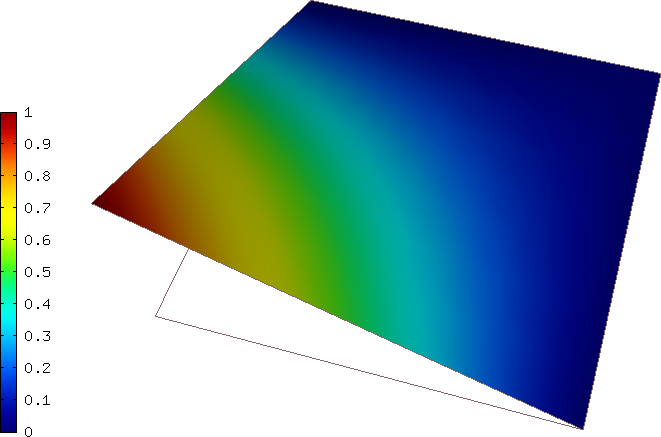
\includegraphics[width=.32\textwidth]{vtx}\hspace{.01\textwidth}
  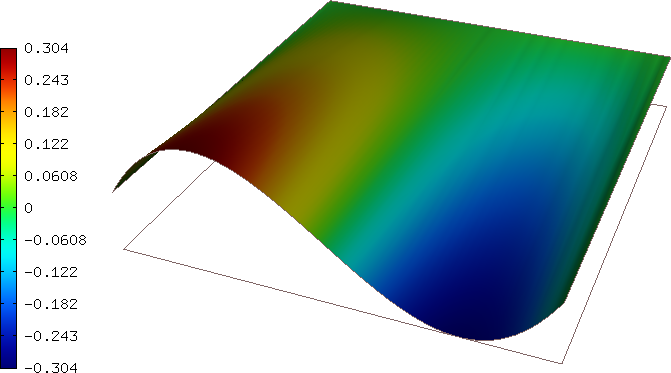
\includegraphics[width=.32\textwidth]{face}\hspace{.01\textwidth}
  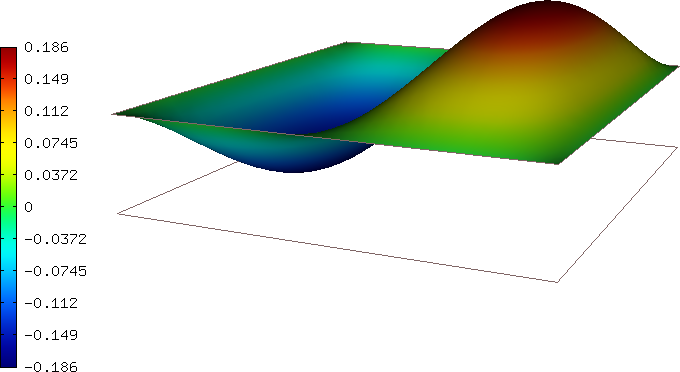
\includegraphics[width=.32\textwidth]{bubble}
  \caption{Shape functions of type (a), (b), (c).}
 	\label{fig:bazep}
\end{figure}

Note that the local approximation subspaces associated with each quadrilateral element might possess different
approximation orders in the lateral and longitudinal direction. Moreover, approximation orders may also vary from
element to element, i.e. for each $g$, $\Space_{hp}^g$ is decomposed into
\begin{equation}\label{eq:hermes_space}
	\Space_{hp,\tau}^g = \{v_{hp}^g \circ\, \mathfrak{r}^g \in
	\mathcal{P}_{p(\elem^g)}(\hat{\elem})
	\},\quad \elem^g\in\mesh^g,
\end{equation}
the local approximation subspaces constructed so that the minimum rule for $H^1$-conforming approximations
(\cite[\S3.5.5]{Hermes-book1}) -- namely that the approximation order of these subspaces coincides with the
approximation order in element interiors (thus constraining the polynomial degree of the edge shape functions during
assembling) -- is satisfied. We will henceofth identify an element with the local approximation subspace
constructed on top of it, so that we can speak of element orders, etc.

Lastly, hanging nodes (mesh vertices in edge interiors) are also
allowed in $\mesh^g$ for greater flexibility of mesh adaptivity (and $H^1$ conformity recovered by additional constraints on the edge shape functions as
described in \cite[\S3.6]{Hermes-book1} and \cite{Hermes-hanging-nodes}).

\subsection{Multimesh assembling}
We are now ready to describe the basic principle of the multimesh assembling algorithm. This has been nicely done in 
the original paper \cite{Hermes-thermoelasticity} (which we will closely follow) but we include the brief description
here as well as it is directly related to one of author's own contributions to Hermes2D described in
\sref{sec:hermes_dg}.

In order to assemble mixed integrals of type \eqref{eq:mixed_int}, the assembling procedure works with a geometrical union $\mesh[h,u]$ of all meshes $\mesh^1$, $\mesh^2$, $\mesh^3$. This union is never 
explicitly created in memory.
Rather, its virtual elements are traversed by the usual element-wise assembling loop. Let $\widetilde\elem \in \mesh[h,u]$
be the currently visited virtual element. As all meshes $\mesh^g$ originate from a common master mesh, there is for each
$g$ exactly one element $\elem^g\in\mesh^g$ such that $\widetilde\elem^g\subset \elem^g$ is the \textit{sub-element} of 
$\elem^g$ (which is called in this context the \textit{active element} on $\mesh^g$) corresponding to $\widetilde\elem$.
\begin{figure}[!hb]
  \centering
  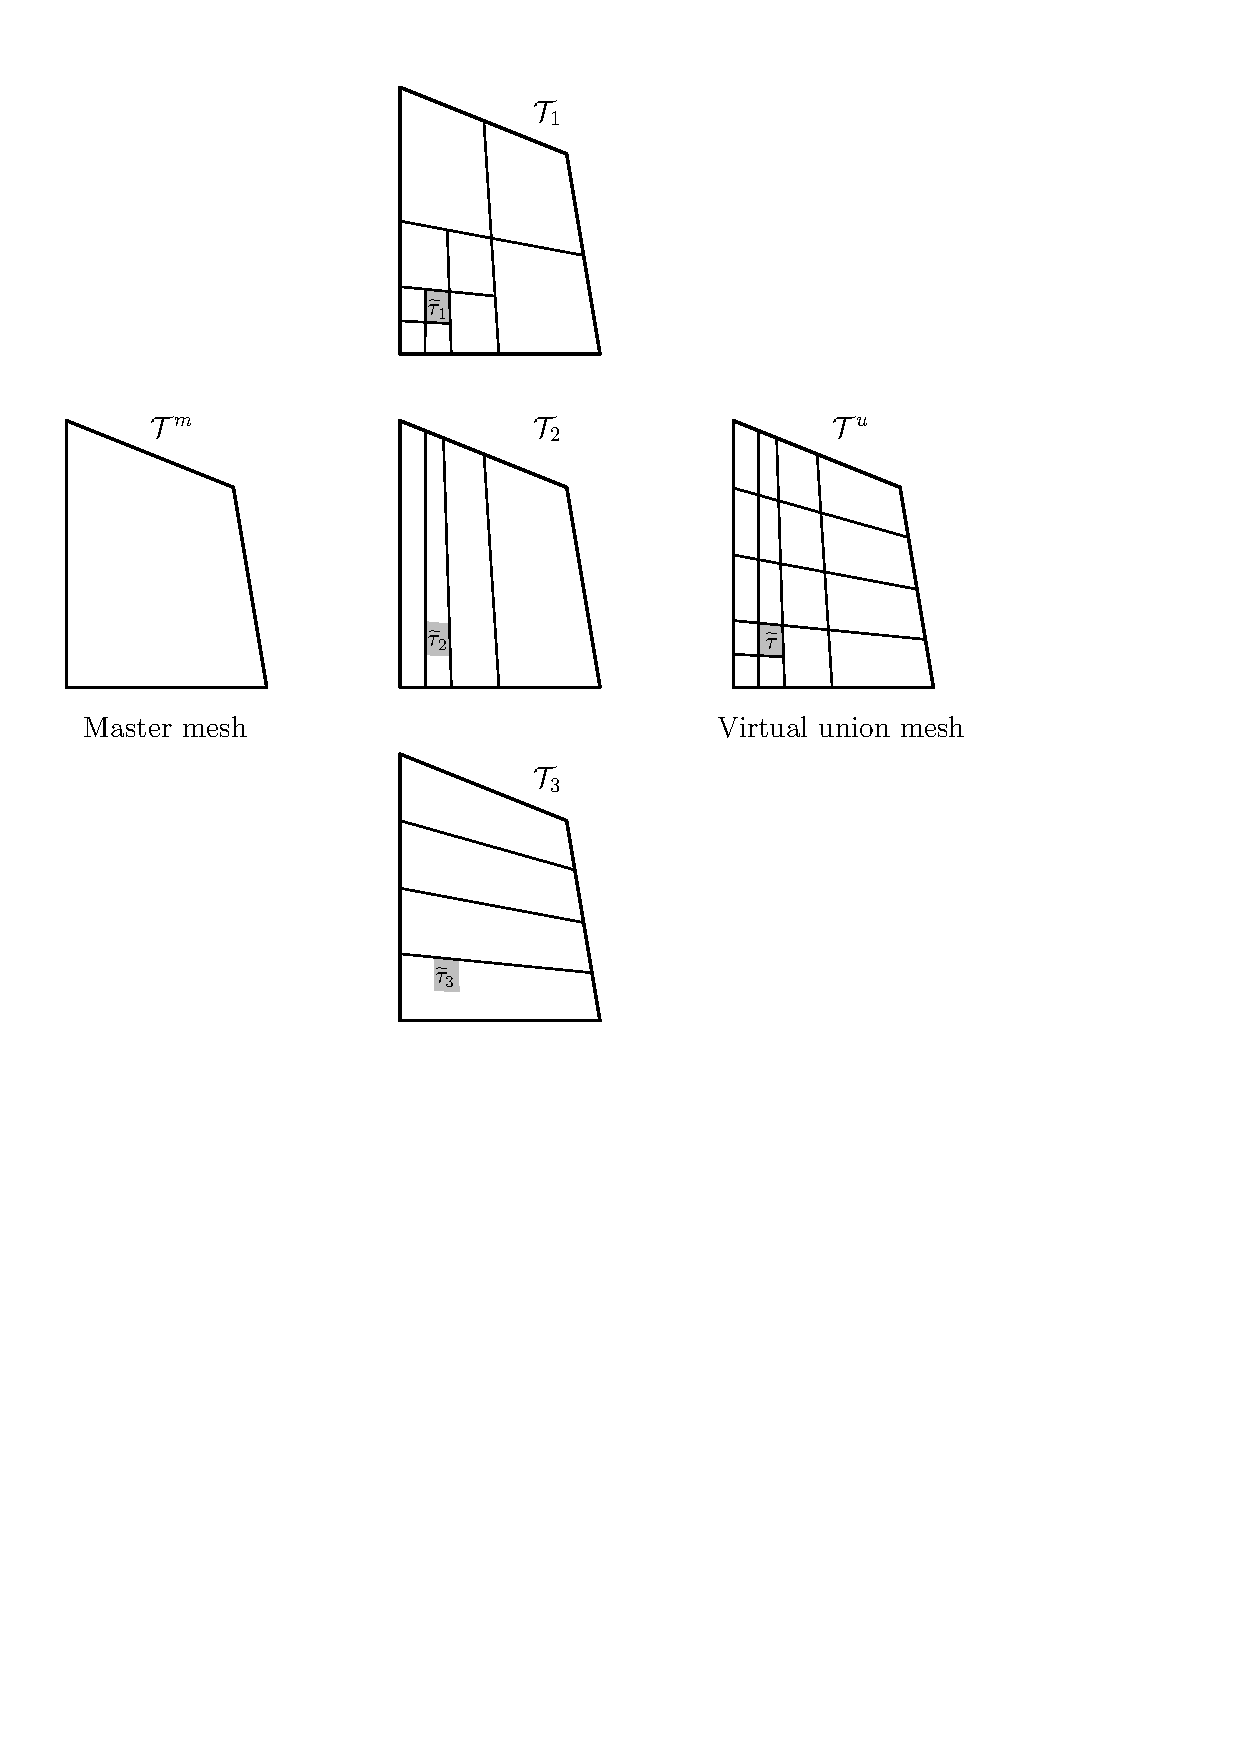
\includegraphics[scale=.9]{multimesh}
  \caption[Multimesh assembling]{One state of the multimesh assembling algorithm. Note that the sub-element mapping
  $\mathfrak{s}^1$ is identity.}
 	\label{fig:multimesh}
\end{figure}

To evaluate the integrals comprising the weak formulation of the problem (recall Prb. \ref{prb:sp3bis}), each
sub-element needs to be transformed to the reference element where the appropriate quadrature points are defined.
While for the active element on $\mesh^g$, the referece mapping $\mathfrak{r}^g(\elem^g) = \hat{\elem}$ as required, it
transforms the sub-element to a subset $\mathfrak{r}^g(\widetilde\elem^g) \subset \hat{\elem}$. Thus another mapping
$\mathfrak{s}^g : \hat{\elem} \to \hat{\elem}$ is introduced (the \textit{sub-element mapping}) such that
$\mathfrak{s}^g(\mathfrak{r}^g(\widetilde\elem^g)) = \hat{\elem}$. These two mappings allow Hermes2D to evaluate all
integrals in the weak forms by using elements only on the mesh on which the integrands live, thus incurring no further
error beyond the inevitable one of numerical integration.

\subsection{Discontinuous Galerkin assembling}\label{sec:hermes_dg}
As a joint effort of the author of this thesis and Luk{\' a}{\v s} Korous, at this moment (November 2014) the main
developer of the Hermes2D project, Hermes2D has been enabled for discontinuous Galerkin approximation of
variational problems. This involved the extension of the assembly procedure to
perform surface integration over all edges of all elements for user-defined discontinuous Galerkin bilinear and linear
forms and also exposing for these forms the access to shape functions and geometrical information of both elements sharing a
common interface (thus allowing the user to define interface operators like $\jump{\cdot}$ and $\langle\cdot\rangle$ introduced in
 \sref{sec:DGM}). 
 Because of the possibility of hanging nodes in the mesh (essentially needed for efficient mesh
 refinement), the actual integration of these forms along element edges is non-trivial as matching points
 from both sides of the edge need to be correctly determined.  
This functionality has been implemented in the class \lstinline{NeighborSearch} based on the same fundamental idea
underlying the multimesh assembling (namely that of sub-element mappings).

The \lstinline[basicstyle=\ttfamily]{NeighborSearch} class characterizes a neighborhood of a given edge in terms of adjacent
elements and provides methods for getting limit values of discontinuous functions from both sides of the edge. Each instance of the
class is connected to a mesh and its active element. The current active element becomes the \textit{central element} of
the neighborhood and all adjacent elements the \textit{neighbors}. In order to search for the neighboring elements, one
selects a particular edge of the central element and calls a function that enumerates the neighbors and fills in the
array of sub-element mappings (transformations) neccessary for getting function values at matching quadrature points
from both sides of the selected (active) edge.
The actual procedure depends on the relative size of the central element with respect to the neighbor element(s) across
the active edge:
\begin{itemize}
  \item If active edge is shared by two elements of same size, then the neighboring element is identified directly and 
  no additional transformations are needed to obtain values of any given function from either side of active edge.
\begin{figure}[!h]
  \centering
  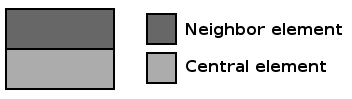
\includegraphics[scale=.45]{no_trans}
  \caption{Neighbor search -- ``no transformation'' case}
\end{figure}
  
  \item If the neighbor element is bigger than the central element, then we "go up" on the central element, until we
  find its parent that has the same size as the neighbor. We keep track of the visited intermediate parents and after 
  the final one has been found (in the ultimate case an element of the master
  mesh), we use them in reverse order to fill in the sub-element mapping array. These
  transformations will be applied to integration points used when integrating a function on the neighboring
  (bigger) element in order to obtain values at points matching those from the central element's side.
  
\begin{minipage}{\linewidth}
    \centering
    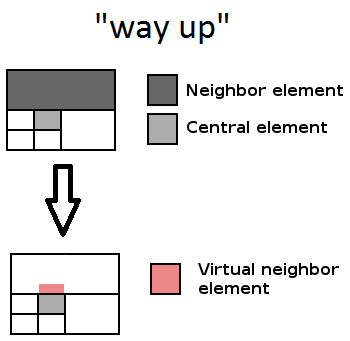
\includegraphics[scale=.6]{way_up2}
    \captionof{figure}{Neighbor search -- ``way up'' case}
\end{minipage}
  
  \item If the neighbor element is smaller than the central element, it means that it is one of several neighbors across
  the active edge. Hence, we "go down" in the central element in order to find a (virtual) sub-element matching the 
  currently processed neighbor and store the corresponding transformations in the neighbor's row of the
  (two-dimensional) array of sub-element mappings. This way, we obtain for each neighbor a set of
  transformations which will be applied on the central element to transform integration points to the correct
  sub-element matching the neighbor.

\begin{minipage}{\linewidth}
    \centering
    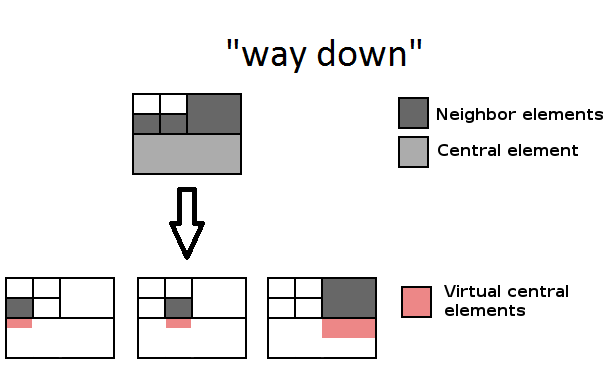
\includegraphics[scale=.6]{way_down2}
    \captionof{figure}{Neighbor search -- ``way down'' case}
\end{minipage}

\end{itemize}

If only an external function is supposed to be discontinuous across the active edge (e.g. in the case of assembling
linear forms), an appropriate \linebreak\lstinline[basicstyle=\ttfamily]{DiscontinuousFunc} object is created for such a
function and exposed to the user who can use it to retrieve actual values at the matching integration points from both
sides of the active segment.

If also the trial and test functions need to be considered discontinuous (e.g when assembling DG bilinear forms), the
local approximation bases (called \textit{shapesets} in Hermes2D) on the central element and on the current
neighbor element are extended by zero to the whole neighborhood of the two elements.
The so-called \textit{extended shapeset} thus created is 
queried during assembling for the count of all contained extended shape functions and their global DOF (degree of
freedom) numbers.
Assembling is done over all these extended shape functions -- the currently processed trial and test functions
is exposed to the user again as
\lstinline[basicstyle=\ttfamily]{DiscontinuousFunc} objects with the shape functions' values (and derivatives) at
integration points at both sides of active edge.
  
This procedure is limited by the requirement that the number of integration points at both sides of
active edge is the same. This is enforced artificially during assembling by performing the integrations of DG interface
forms using a quadrature of the maximal supported order. Note that this does not restricts the approximation spaces
in any way -- it only pertains to the numerical integration.

\section{$hp$-adaptivity}\label{sec:hermes_adapt}
The goal of the $hp$-adaptivity process is to combine spatial subdivision of selected elements ($h$-refinement) with
local increase of their approximation order ($p$-refinement) so that the total available number of degrees of freedom at given stage of
the process is utilized most efficently (i.e., relatively big number of low-order elements is used in regions with highly oscillating solution
while smaller number of high-order elements in regions with smoother solution behavior). As there are many
possible combinations of $h$ and $p$ refinements of given element, one number per element provided by traditional
a-posteriori error estimates for FEM is insufficient to guide the $hp$ adaptivity. Instead, a robust
approach to local error estimation is used in Hermes2D that is based on comparing two
solutions of different approximation orders (note that this technique has been used for a long time for solving the
ordinary differential equations). This allows to determine the whole shape of the approximation error $e = u - u_{hp}$ 
over each element and use it to determine the best refinement candidate that decreases the total approximation error for
the lowest number of added DOF. 

For illustration, let us consider the general approximate problem \ref{prb:general}, coming from the corresponding
exact variational problem with solution $\U\in\mathbb{H}^1(\VV)$.

To understand the $hp$-adaptivity algorithm in the multimesh setting, we must realize that the approximation error is a
vector field with components corresponding to  is characterized by the following steps (which will be commented in more
detail below)

\begin{enumerate}
	\item approximate $\flfl$ on current set of spaces $\Space_{hp}^g$ to obtain $\flfl_{hp}$
	\item global refinement: $\Space_{hp}^g \to \Space_{h/2,p+1}^g$, obtain $\flfl_{h/2,p+1}$
	\item set $\flfl_{\rf} = \flfl_{h/2,p+1}$, compute $\indic^g_\elem = \norm[\elem,g]{\fl_{hp}^g-\fl^g_{\rf}}^2$ for
	each element $\elem^g \in \mesh^g$; here  
	\item accumulate $\indic_{hp,\elem}^g$ from all meshes $\tau^g$ to obtain
	$E_{hp}=\tzterm{norm}{\norm{\flfl_{hp}-\flfl_{\rf}}}$ ~~\gray{\footnotesize (note that $\norm{E_{hp}}^2 = \sum_g\sum_{K_n^g\in\tau^g}\indic^g_n$ where $\indic^g_n = \norm[n,g]{\fl_{hp}^g-\fl^g_{\rf}}^2$)}
	%                \gray{\footnotesize (by accumulating error estimates from all $K_n^g\in\tau^g$)}
	\item stop if $\frac{E_{hp}}{\norm{\flfl_{\rf}}} \leq TOL$, otherwise
	\item mark elements $K_n^g$ for which $\frac{\indic^g_n}{\tzterm{normelem}{\norm[n,g]{\fl_{\rf}^g}}} > \theta\max_{n',g'}\frac{\indic^{g'}_{n'}}{\norm[n',g']{\fl_{\rf}^{g'}}}$
	\item decide refinement strategy ($h$-, $p$-, iso/anisotropic, etc.)  
	\item refine marked elements ($\Space_{hp}^g \to V_{h'p'}^g$)
\end{enumerate}

Note that $\indic_g$ 
  %\chapter{Coupled code system for quasi-static whole-core calculations}\label{chap:coupled}

For the purposes of the project\footnote{
Project TA01020352 -- Increasing utilization of nuclear fuel through optimization of an inner fuel cycle and
calculation of neutron-physics characteristics of nuclear reactor cores. Principal investigators: R. {\v C}ada
(University of West Bohemia) and J. Rataj (Czech Technical University} 
whose target is an in-core fuel management code for nuclear
reactors\footnote{ primarily of the pressurized type (i.e. without coolant boiling during operational conditions) but with arbitrary fuel
assembly geometry, thus applicable to both major designs in use worldwide -- the Russian WWER reactors as well as the
US PWR reactors.}, the author developed a full three-dimensional multigroup neutron diffusion solver based on the finite
element discretization described in previous chapters. Its first responsibility is to solve the core criticality problem
for given input data (macroscopic cross-sections) defined by the proposed fuel loading pattern, i.e. to solve the
generalized eigenvalue problem
$$
	\mat{A}\mat{x} = \lambda\mat{B}\mat{x}
$$
for $\lambda$ of smallest magnitude. Refering to \sref{sec:criticality} (Remark \ref{rem:keff}), $\lambda =
\frac{1}{\keff} \approx 1$ for a (nearly) critical state. We also recall from \alert{ref} that in a general multigroup
setting, the matrices are non-symmetric and $\mat{B}$ is a singular matrix with zero rows corresponding to low-energy
groups.

It is written in Python 2.7 with critical parts (typically where loops over mesh cells are needed) in C++ as SWIG
extension modules. FE matrix assembly is handled by the well-established open-source system FEniCS \cite{dolfin1,
dolfin2} and its linear algebra backend PETSc \cite{petsc1}. PETSc library and its fork focusing on solving large sparse
eigenvalue problems, SLEPc \cite{slepc1}, is also primarily used for solving the assembled systems. This has the
advantage that parallel assembly and solution using the MPI protocol is almost automatic (provided an appropriate
solver/preconditioner is being used).
FEniCS also makes it easy to pass arguments directly to the linear-algebra backend, thus facilitating for the user the
selection of algebraic solver and its properties. 

In the benchmarks below, we found the most robust setting to be the combination of a Jacobi-Davidson generalized
eigensolver (\cite{slepcjd}) with a PETSc implementation of BiCGStab(\ell) \cite{Sleijpen1} as an inner solver (using
the default $\ell = 2$). It has been demonstrated already in \cite{Sleijpen1} (and analyzed in many later papers, see
e.g. \citer{Notay} and references therein) that the Jacobi-Davidson method is remarkably robust with respect to accuracy
of the solution of the inner solution phase. Therefore, by setting a fixed number of inner iterations to 20 and
employing a smoothed aggregation algebraic multigrid preconditioner with 1 pre- and 1 post-smoothing Richardson
iterations, we were able to get solutions fast enough.

  %\chapter{}\label{chap:evc}

\chapter{Conclusions}

%: ----------------------- bibliography ------------------------

%\begin{multicols}{2} % \begin{multicols}{ # columns}[ header text][ space]
%\begin{tiny} % tiny(5) < scriptsize(7) < footnotesize(8) < small (9)

%\addcontentsline{toc}{chapter}{Bibliography}
%\bibliographystyle{alphaurl}
\bibliographystyle{plainnat} % Title is link if provided
\renewcommand{\bibname}{Literature} % changes the header; default: Bibliography

\bibliography{literature} % adjust this to fit your BibTex file

%\end{tiny}
%\end{multicols}

\appendix
\makeatletter
\@addtoreset{theorem}{chapter}% Reset theorem counter with stepping of chapter
\@addtoreset{lemma}{chapter}% Reset theorem counter with stepping of chapter
\@addtoreset{remark}{chapter}% Reset theorem counter with stepping of chapter
\makeatother
\renewcommand\thetheorem{\thechapter.\arabic{theorem}}
\renewcommand\thelemma{\thechapter.\arabic{lemma}}
\renewcommand\theremark{\thechapter.\arabic{remark}}
\renewcommand\thecorollary{\thechapter.\arabic{corollary}}
\setcounter{theorem}{0}
\setcounter{lemma}{0}
\setcounter{remark}{0}
\setcounter{corollary}{0}

\chapter{Spherical harmonics}\label{app:SH}
The (complex)
spherical harmonic function of degree $n$ and order $m$\\ ($n\in\mathbb{N}_0,\ m\in\mathbb{Z}, 0\leq \abs{m} \leq n$) 
is defined as
\begin{equation}\label{eq:Ynm}
\nomenclature[a]{$\Y{n}{m}$}{spherical harmonic function of degree $n$ and order $m$\nomrefeq}
    \Y{n}{m}(\bomega) = \Y{n}{m}(\polar,\azimuthal) = 
    \sqrt{\frac{2n+1}{4\pi}\frac{(n-m)!}{(n+m)!}} \P{n}{m}(\cos\polar)e^{i m \azimuthal},
\end{equation}
or (since the dependence on polar angle $\polar$ is only through its cosine)
$$
	\Y{n}{m}(\mu,\azimuthal) = \sqrt{\frac{2n+1}{4\pi}\frac{(n-m)!}{(n+m)!}} \P{n}{m}(\mu)e^{i m \azimuthal},
$$
where
\begin{equation}\label{eq:associated_Pn}
    \nomenclature[a]{$\P{n}{m}(\mu)$}{associated Legendre polynomial of degree $n$ and order $m$\nomrefeq} 
    \P{n}{m}(\mu) = 
    \begin{cases} 
    	(-1)^m\sqrt{(1-\mu^2)^m}\ \der[m]{\P{n}(\mu)}{\mu} & \mbox{if } \hphantom{-}\,0 \leq m \leq n,\\[.5em]
    \displaystyle (-1)^{-m}\frac{(n+m)!}{(n-m)!}\P{n}{-m}(\mu) & \mbox{if } -n \leq m < 0 
    \end{cases}
\end{equation}
are the \textit{associated Legendre functions}. Note that ordinary Legendre polynomials are recovered for $m = 0$. 

These functions form a closed orthonormal system on $\Lp{2}(\Sphere)$ with respect to the standard inner product
$$
(\psi, \varphi)_{\Lp[2](\Sphere)} = \intA{\psi(\bomega) {\overline\varphi(\bomega)}}
$$
(where the overline denotes complex conjugation), that is
$$
\begin{aligned}
\intA{\Y{n}{m}(\bomega)\Yc{n}{m}(\bomega)} &=
\int_{0}^{2\pi}\d{\azimuthal}\int_{0}^{\pi}\sin\polar\d{\polar}  
\Y{n}{m}(\polar,\azimuthal)\Yc{l'}{m'}(\polar,\azimuthal)\\[.25em]
& = \int_{0}^{2\pi}\d{\azimuthal}\int_{-1}^{1}\d{\mu}
\Y{n}{m}(\mu,\azimuthal)\Yc{l'}{m'}(\mu,\azimuthal) = \kron{m}{m'}\kron{n}{l'}
\end{aligned}
$$
where $\kron{i}{j} = 1$ if $i = j$ and $\kron{i}{j} = 0$ otherwise (Kronecker delta symbol).

A real basis of spherical harmonics can be obtained from complex linear combination of the original basis and can be
written in the following form:
\begin{gather*}
    \sqrt{2}\y{n}{m}(\polar,\azimuthal) = 
    \pw{C_n^m \P{n}{m}(\cos\polar)\cos(m \azimuthal) = \mathrm{Re}\Y{n}{m}(\polar,\azimuthal)}{$m\geq 0$}
    {C_n^{-m} \P{n}{-m}(\cos\polar)\sin(-m \azimuthal) = \mathrm{Im}\Y{n}{-m}(\polar,\azimuthal)}{$m < 0$,}\\
    C_n^m = \sqrt{\frac{2n+1}{4\pi}\frac{(n-m)!}{(n+m)!}}.
\end{gather*}
Functions $\y{n}{m}$ are usually called \textit{tesseral spherical harmonics of degree $n$ and order $m$} (sometimes the
case $n = m$ is distinguished as \textit{sectorial spherical harmonics}). Linear combination of tesseral spherical
harmonics of degree $n$ produces a \textit{surface spherical harmonic of degree $n$}:
\begin{equation*}
\begin{multlined}
    \mathcal{Y}_n(\bomega) = \mathcal{Y}_n(\polar,\azimuthal) = \\A_0 P_n(\cos\polar) + \suma[m]{1}{n}\left[ A_m
    \cos(m\azimuthal)\P{n}{m}(\cos\polar) + B_m \sin(m\azimuthal)\P{n}{m}(\cos\polar)\right]
  \end{multlined}
  \end{equation*}
Surface spherical harmonics are formally defined as restrictions of homogeneous harmonic polynomials of degree $n$ to
unit sphere $\Sphere$ (\cite[Art. 110]{Byerly}, \cite[Def. 3.22]{Schreiner}).

\newpage
\begin{sidewaysfigure}
	\centering
		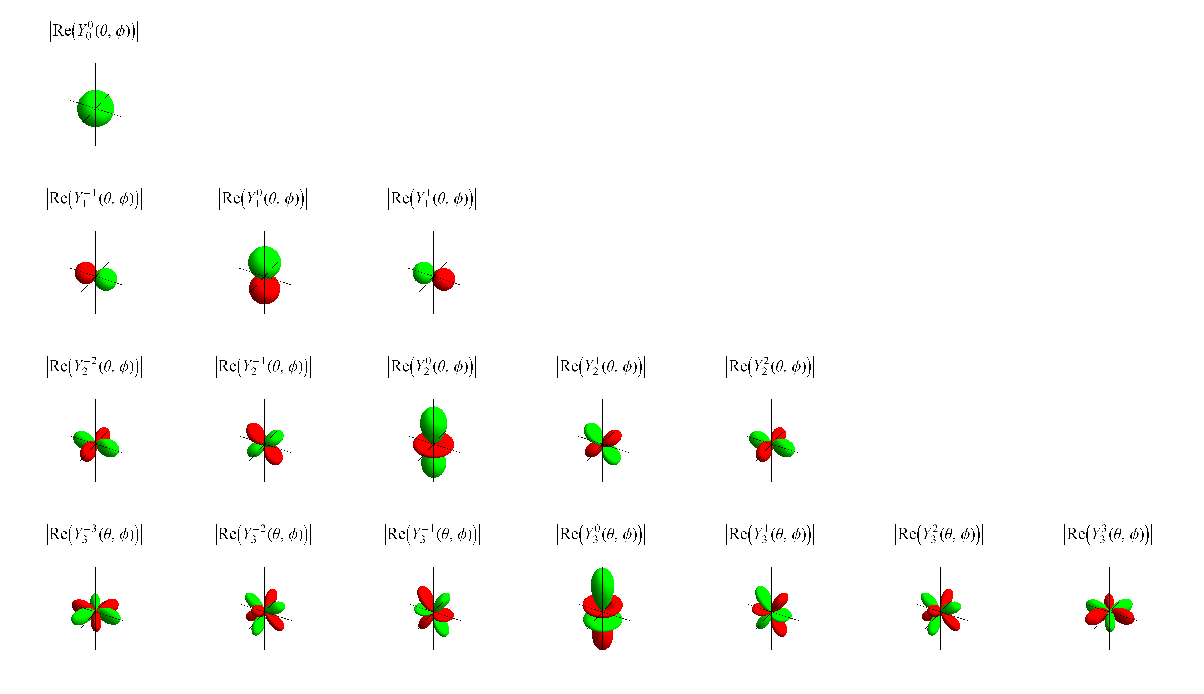
\includegraphics[scale=1.2]{pic/sh.eps}
		\caption[Spherical harmonics]{Spherical harmonics up to $3^{\mbox{rd}}$ degree, plotted in spherical coordinates 
		as specified in the labels above the graphs and colored green if $\mathrm{Re}\,\Y{n}{m} \geq 0$ and red
		otherwise (picture generated by Mathematica 7.0).}%
	\label{fig:SH} 
\end{sidewaysfigure}




%\chapter{Lack of rotational invariance of the $\SN$ advection-reaction operator}

\begin{theorem*}\label{thm:commut_NTE}
Let $L : V\to V$ be the advection-collision operator of the NTE satisfying
$RL = LR$ for all $R\in\mathrm{SO}(3)$. 
Then the corresponding $\SN$ approximation operator
\begin{equation}\label{eq:sn_op_app}
	\Projop[S_N]\op{L}\Projop[S_N]
\end{equation}
(with $\Projop[S_N]$ defined by \eqref{eq:proj_sn}, \eqref{eq:map_SN}, \eqref{eq:map_SN_inv} and particular
ordinates and quadrature sets \mbox{$\omega = \{\bomega_n\}_{\idxset{M}}$, $\mathcal{W} = \{w_n\}_{\idxset{M}}$})
satisfies $$
\op{R}\op{L}\Projop[S_N] = \op{L}\Projop[S_N]\op{R}\quad \forall R\in\mathrm{SO}(3)
$$
if and only if
\begin{equation}\label{eq:thm1_cond}
	\forall n\in \idxset{M}\ \exists m\in\idxset{M}: \mat{R}\bomega_n = \bomega_m \quad \forall \mat{R}\in\mathrm{SO}(3).
\end{equation} 
\end{theorem*}
\begin{remark*}
	Note that the conditions \eqref{eq:thm1_cond} can be satisfied only in the limit \mbox{$M\to\infty$}.
\end{remark*}
\begin{proof}
First, recall from \sref{sec:opsn} that for any $\SN$ approximate function \mbox{$f_{S_N}\in V_{S_N}$}, 
$$
	\Projop[SN]f_{S_N} = f_{S_N}.
$$
Also, for $\psi_{S_N} \in V_{S_N}$:
$$
	\bomega\cdot\nabla\psi_{S_N}(\br,\bomega) = \left.\pw{
		\bomega_n\cdot\nabla\psi(\br,\bomega_n)}{if $\bomega = \bomega_n$ for $\bomega_n\in\omega$}
		{0}{if $\bomega \not \in \omega$.}\right\} \in V_{S_N}
$$
where we recall the characterization of $V_{S_N}$ as a space of functions that, as functions of $\bomega$, vanish
everywhere on $\Sphere$ except points corresponding to the selected ordinates set. Therefore for $\psi_{S_N} \in
V_{S_N}$, 
$$
	L\psi_{S_N} \equiv \bomega\cdot\nabla\psi_{S_N} + \sigma_t\psi_{S_N} \in V_{S_N}.
$$
Since \mbox{$\Rng (\PiSN) = V_{S_N}$}, it follows that the $\SN$ operator \eqref{eq:sn_op_app} can be simplified as:
\begin{equation}\label{eq:sn_op2}
	\Projop[S_N]\op{L}\Projop[S_N] = \op{L} \Projop[SN].
\end{equation}
Because of the commutativity of $L$ and $R$, it therefore suffices to show that $\Projop[S_N]$ commutes
with $\op{R}$, that is (using def. \eqref{eq:proj_sn})
\begin{equation}\label{eq:thm1_point}
	R \PiSN \PihSN \psi = \PiSN \PihSN R \psi\quad  \forall \psi \in V, 
\end{equation}
if and only if the condition \eqref{eq:thm1_cond} holds.\\[.2em] 

As in \sref{sec:opsn}, we will suppress the spatial dependence as the $\SN$ approximation concerns only the angular
dependence. For any $\psi\in V$, we have
\begin{equation*}
	\PihSN R\psi(\bomega) = \colset{R\psi(\bomega_n)}{\idxset{M}} = \colset{\psi(\mat{R}^T\bomega_n)}{\idxset{M}}.
\end{equation*}
Applying $\PiSN$ thus yields a function $f_\psi = \PiSN\PihSN R\psi \in V_{S_N}$ such that
\begin{equation}\label{eq:thm1_f}
f_\psi(\bomega) = \pw{\psi(\mat{R}^T\bomega_n)}{if $\bomega = \bomega_n$ for $\bomega_n\in\omega$}{0}{if $\bomega \not
	\in \omega$.}
\end{equation}
On the other hand, let $u = \PiSN\PihSN\psi$. Then
$$
u(\bomega) = \pw{\psi(\bomega_n)}{if $\bomega = \bomega_n$ for $\bomega_n\in\omega$}{0}{if $\bomega \not
	\in \omega$}
$$ 
and the rotated function $g_\psi(\bomega) = R\PiSN\PihSN\psi = R u(\bomega)$ is given by
$$
g_\psi(\bomega) = u(\mat{R}^T\bomega) = \pw{\psi(\bomega_n)}{if $\mat{R}^T\bomega = \bomega_n$ for
$\bomega_n\in\omega$}{0}{if $\mat{R}^T\bomega \not \in \omega$}
$$
or, equivalently, by
\begin{equation}\label{eq:thm1_g}
g_\psi(\bomega) = \pw{\psi(\bomega_n)}{if $\bomega = \mat{R}\bomega_n$ for
$\bomega_n\in\omega$}{0}{if $\bomega \not \in \mat{R}\omega$}
\end{equation}
(where action of $\mat{R}$ on the set $\omega$ is understood element-wise). If the ordinate set $\omega$ contains for
any ordinate $\bomega_n$ also its rotated copy $\mat{R}\bomega_n$, i.e., condition \eqref{eq:thm1_cond} holds, then also
$$
	\bomega_n = \mat{R}^T\bomega_m
$$
and after simple substitution in \eqref{eq:thm1_g} and renumbering in \eqref{eq:thm1_f}, we obtain
$$
	f_\psi(\bomega) = g_\psi(\bomega).
$$
In order for this equality to hold true for any $\psi \in V$ (and hence for \eqref{eq:thm1_point} to hold true), the
condition \eqref{eq:thm1_f} is also necessary.
\end{proof}
\comment{
\begin{theorem}\label{thm:commut_NTE2}
Let $K : V\to V$ be the transfer operator of the NTE satisfying
$RK = KR$ for all $R\in\mathrm{SO}(3)$. 
Then the corresponding $\SN$ approximation operator
\begin{equation}\label{eq:sn_op_app}
	\Projop[S_N]\op{K_{S_N}}\Projop[S_N]
\end{equation}
where $\op{K}_{S_N}: V_{S_N} \to V$ is defined by
$$
	\op{K}_{S_N} f(\bomega) = \sum_{n=1}^{M} w_n\kappa(\bomega\cdot\bomega_n) f(\bomega_n), \quad \bomega_n\in \omega,\
	w_n\in \mathcal{W} $$
(and definitions of $\Projop[SN]$, $\omega$, $\mathcal{W}$ are as in previous theorem),  satisfies
$$
\op{R}\Projop[S_N] \op{K}_{S_N}\Projop[S_N] = \Projop[S_N] \op{K}_{S_N}\Projop[S_N]\op{R}\quad \forall
R\in\mathrm{SO}(3) $$
if and only if the condition \eqref{eq:thm1_cond} of Thm. \ref{thm:commut_NTE} holds.
\end{theorem}
\begin{proof}

\end{proof}
}

\chapter{$\PN[3]$ advection matrices}\label{app:C}
\comment{
Recall from \sref{sec:pn_op} that the steady-state $\PN$ system can be written in the operator form as follows (eq.
\eqref{eq:pn_op}):
\begin{equation}\label{eq:PN_ss_app}
	\PihPN (A+\Sigma_t-K) \PiPN\Phi = \PihPN q,
\end{equation}
where (in the monoenergetic case) 
$$
\begin{gathered}
A\psi(\br,\bomega) = \bomega\cdot\nabla\psi(\br,\bomega),\quad
\Sigma_t\psi(\br,\bomega) = \sigma_t(\br)\psi(\br,\bomega)\\
K\psi(\br,\bomega) = \intA[']{\kappa(\br,\bomega\cdot\bomega')\psi(\br,\bomega')}.
\end{gathered}         
$$
and for $\mat{F} = \col \{f_k\}_{\idxset{K}}$,
\begin{equation}\label{eq:pn_op_def_app}
\bigl(\PiPN\mat{F}\bigr)(\bomega) := \sum_{k=1}^{ K} f_k\Y{k}{}(\bomega), \quad
\PihPN f(\bomega) = \col \left\{(f, \Y{k}{})_{\Lp[2](\Sphere)}\right\}_{\idxset{K}}
\end{equation}
}
In this appendix, we investigate the advection matrices $\mat{A}_{P_N}^s$ ($s = x,y,z$) for the special case $N = 3$ 
(the statements that follow have been computationally verified to hold for $N = 1,2,\ldots,11$ using the symbolic 
system Mathematica 9.0).
It is more convenient for this analysis to consider the steady-state $\PN$ equations \eqref{eq:PN_ss_app} as a limit
of the time-dependent equations
\begin{equation}\label{eq:PN_ss_app}
	\PihPN \left(\pd{}{t} + A + \Sigma_t - K\right) \PiPN\Phi = \PihPN q,
\end{equation}
in which $\pd{\psi}{t} \to 0$, for time-independent boundary conditions and sources
\linebreak[4]\mbox{$q(\cdot,\cdot,t) = \text{const}$}.
Then, the advection matrices describe advection of neutrons introduced into the system by the boundary and internal
sources, which is in the steady-state limit perfectly balanced by their attenuation due to net effect of collisions of
all types.

$$
\scriptsize
\hspace*{-2cm}
\begin{aligned}
\mat{A}_{P_N}^x &=
\left[
\begin{array}{cccccccccccccccc}
 0 & 0 & 0 & \frac{1}{\sqrt{3}} & 0 & 0 & 0 & 0 & 0 & 0 & 0 & 0 & 0 & 0 & 0 & 0 \\
 0 & 0 & 0 & 0 & \frac{1}{\sqrt{5}} & 0 & 0 & 0 & 0 & 0 & 0 & 0 & 0 & 0 & 0 & 0 \\
 0 & 0 & 0 & 0 & 0 & 0 & 0 & \frac{1}{\sqrt{5}} & 0 & 0 & 0 & 0 & 0 & 0 & 0 & 0 \\
 \frac{1}{\sqrt{3}} & 0 & 0 & 0 & 0 & 0 & -\frac{1}{\sqrt{15}} & 0 & \frac{1}{\sqrt{5}} & 0 & 0 & 0 & 0 & 0 & 0 & 0 \\
 0 & \frac{1}{\sqrt{5}} & 0 & 0 & 0 & 0 & 0 & 0 & 0 & \sqrt{\frac{3}{14}} & 0 & -\frac{1}{\sqrt{70}} & 0 & 0 & 0 & 0 \\
 0 & 0 & 0 & 0 & 0 & 0 & 0 & 0 & 0 & 0 & \frac{1}{\sqrt{7}} & 0 & 0 & 0 & 0 & 0 \\
 0 & 0 & 0 & -\frac{1}{\sqrt{15}} & 0 & 0 & 0 & 0 & 0 & 0 & 0 & 0 & 0 & \sqrt{\frac{6}{35}} & 0 & 0 \\
 0 & 0 & \frac{1}{\sqrt{5}} & 0 & 0 & 0 & 0 & 0 & 0 & 0 & 0 & 0 & -\sqrt{\frac{3}{35}} & 0 & \frac{1}{\sqrt{7}} & 0 \\
 0 & 0 & 0 & \frac{1}{\sqrt{5}} & 0 & 0 & 0 & 0 & 0 & 0 & 0 & 0 & 0 & -\frac{1}{\sqrt{70}} & 0 & \sqrt{\frac{3}{14}} \\
 0 & 0 & 0 & 0 & \sqrt{\frac{3}{14}} & 0 & 0 & 0 & 0 & 0 & 0 & 0 & 0 & 0 & 0 & 0 \\
 0 & 0 & 0 & 0 & 0 & \frac{1}{\sqrt{7}} & 0 & 0 & 0 & 0 & 0 & 0 & 0 & 0 & 0 & 0 \\
 0 & 0 & 0 & 0 & -\frac{1}{\sqrt{70}} & 0 & 0 & 0 & 0 & 0 & 0 & 0 & 0 & 0 & 0 & 0 \\
 0 & 0 & 0 & 0 & 0 & 0 & 0 & -\sqrt{\frac{3}{35}} & 0 & 0 & 0 & 0 & 0 & 0 & 0 & 0 \\
 0 & 0 & 0 & 0 & 0 & 0 & \sqrt{\frac{6}{35}} & 0 & -\frac{1}{\sqrt{70}} & 0 & 0 & 0 & 0 & 0 & 0 & 0 \\
 0 & 0 & 0 & 0 & 0 & 0 & 0 & \frac{1}{\sqrt{7}} & 0 & 0 & 0 & 0 & 0 & 0 & 0 & 0 \\
 0 & 0 & 0 & 0 & 0 & 0 & 0 & 0 & \sqrt{\frac{3}{14}} & 0 & 0 & 0 & 0 & 0 & 0 & 0 \\
\end{array}
\right]\\[5em]
\mat{A}_{P_N}^y &=
\left[
\begin{array}{cccccccccccccccc}
 0 & \frac{1}{\sqrt{3}} & 0 & 0 & 0 & 0 & 0 & 0 & 0 & 0 & 0 & 0 & 0 & 0 & 0 & 0 \\
 \frac{1}{\sqrt{3}} & 0 & 0 & 0 & 0 & 0 & -\frac{1}{\sqrt{15}} & 0 & -\frac{1}{\sqrt{5}} & 0 & 0 & 0 & 0 & 0 & 0 & 0 \\
 0 & 0 & 0 & 0 & 0 & \frac{1}{\sqrt{5}} & 0 & 0 & 0 & 0 & 0 & 0 & 0 & 0 & 0 & 0 \\
 0 & 0 & 0 & 0 & \frac{1}{\sqrt{5}} & 0 & 0 & 0 & 0 & 0 & 0 & 0 & 0 & 0 & 0 & 0 \\
 0 & 0 & 0 & \frac{1}{\sqrt{5}} & 0 & 0 & 0 & 0 & 0 & 0 & 0 & 0 & 0 & -\frac{1}{\sqrt{70}} & 0 & -\sqrt{\frac{3}{14}} \\
 0 & 0 & \frac{1}{\sqrt{5}} & 0 & 0 & 0 & 0 & 0 & 0 & 0 & 0 & 0 & -\sqrt{\frac{3}{35}} & 0 & -\frac{1}{\sqrt{7}} & 0 \\
 0 & -\frac{1}{\sqrt{15}} & 0 & 0 & 0 & 0 & 0 & 0 & 0 & 0 & 0 & \sqrt{\frac{6}{35}} & 0 & 0 & 0 & 0 \\
 0 & 0 & 0 & 0 & 0 & 0 & 0 & 0 & 0 & 0 & \frac{1}{\sqrt{7}} & 0 & 0 & 0 & 0 & 0 \\
 0 & -\frac{1}{\sqrt{5}} & 0 & 0 & 0 & 0 & 0 & 0 & 0 & \sqrt{\frac{3}{14}} & 0 & \frac{1}{\sqrt{70}} & 0 & 0 & 0 & 0 \\
 0 & 0 & 0 & 0 & 0 & 0 & 0 & 0 & \sqrt{\frac{3}{14}} & 0 & 0 & 0 & 0 & 0 & 0 & 0 \\
 0 & 0 & 0 & 0 & 0 & 0 & 0 & \frac{1}{\sqrt{7}} & 0 & 0 & 0 & 0 & 0 & 0 & 0 & 0 \\
 0 & 0 & 0 & 0 & 0 & 0 & \sqrt{\frac{6}{35}} & 0 & \frac{1}{\sqrt{70}} & 0 & 0 & 0 & 0 & 0 & 0 & 0 \\
 0 & 0 & 0 & 0 & 0 & -\sqrt{\frac{3}{35}} & 0 & 0 & 0 & 0 & 0 & 0 & 0 & 0 & 0 & 0 \\
 0 & 0 & 0 & 0 & -\frac{1}{\sqrt{70}} & 0 & 0 & 0 & 0 & 0 & 0 & 0 & 0 & 0 & 0 & 0 \\
 0 & 0 & 0 & 0 & 0 & -\frac{1}{\sqrt{7}} & 0 & 0 & 0 & 0 & 0 & 0 & 0 & 0 & 0 & 0 \\
 0 & 0 & 0 & 0 & -\sqrt{\frac{3}{14}} & 0 & 0 & 0 & 0 & 0 & 0 & 0 & 0 & 0 & 0 & 0 \\
\end{array}
\right]
\end{aligned}
$$
\newpage
$$
\scriptsize
\hspace*{-2cm}
\mat{A}_{P_N}^z =
\left[
\begin{array}{cccccccccccccccc}
 0 & 0 & \frac{1}{\sqrt{3}} & 0 & 0 & 0 & 0 & 0 & 0 & 0 & 0 & 0 & 0 & 0 & 0 & 0 \\
 0 & 0 & 0 & 0 & 0 & \frac{1}{\sqrt{5}} & 0 & 0 & 0 & 0 & 0 & 0 & 0 & 0 & 0 & 0 \\
 \frac{1}{\sqrt{3}} & 0 & 0 & 0 & 0 & 0 & \frac{2}{\sqrt{15}} & 0 & 0 & 0 & 0 & 0 & 0 & 0 & 0 & 0 \\
 0 & 0 & 0 & 0 & 0 & 0 & 0 & \frac{1}{\sqrt{5}} & 0 & 0 & 0 & 0 & 0 & 0 & 0 & 0 \\
 0 & 0 & 0 & 0 & 0 & 0 & 0 & 0 & 0 & 0 & \frac{1}{\sqrt{7}} & 0 & 0 & 0 & 0 & 0 \\
 0 & \frac{1}{\sqrt{5}} & 0 & 0 & 0 & 0 & 0 & 0 & 0 & 0 & 0 & 2 \sqrt{\frac{2}{35}} & 0 & 0 & 0 & 0 \\
 0 & 0 & \frac{2}{\sqrt{15}} & 0 & 0 & 0 & 0 & 0 & 0 & 0 & 0 & 0 & \frac{3}{\sqrt{35}} & 0 & 0 & 0 \\
 0 & 0 & 0 & \frac{1}{\sqrt{5}} & 0 & 0 & 0 & 0 & 0 & 0 & 0 & 0 & 0 & 2 \sqrt{\frac{2}{35}} & 0 & 0 \\
 0 & 0 & 0 & 0 & 0 & 0 & 0 & 0 & 0 & 0 & 0 & 0 & 0 & 0 & \frac{1}{\sqrt{7}} & 0 \\
 0 & 0 & 0 & 0 & 0 & 0 & 0 & 0 & 0 & 0 & 0 & 0 & 0 & 0 & 0 & 0 \\
 0 & 0 & 0 & 0 & \frac{1}{\sqrt{7}} & 0 & 0 & 0 & 0 & 0 & 0 & 0 & 0 & 0 & 0 & 0 \\
 0 & 0 & 0 & 0 & 0 & 2 \sqrt{\frac{2}{35}} & 0 & 0 & 0 & 0 & 0 & 0 & 0 & 0 & 0 & 0 \\
 0 & 0 & 0 & 0 & 0 & 0 & \frac{3}{\sqrt{35}} & 0 & 0 & 0 & 0 & 0 & 0 & 0 & 0 & 0 \\
 0 & 0 & 0 & 0 & 0 & 0 & 0 & 2 \sqrt{\frac{2}{35}} & 0 & 0 & 0 & 0 & 0 & 0 & 0 & 0 \\
 0 & 0 & 0 & 0 & 0 & 0 & 0 & 0 & \frac{1}{\sqrt{7}} & 0 & 0 & 0 & 0 & 0 & 0 & 0 \\
 0 & 0 & 0 & 0 & 0 & 0 & 0 & 0 & 0 & 0 & 0 & 0 & 0 & 0 & 0 & 0 \\
\end{array}
\right]
$$

By computing the norms of matrices
$$
D_{xy} := \left(\mat{A}_{P_N}^x\right)^T \mat{A}_{P_N}^y - \left(\mat{A}_{P_N}^y\right)^T \mat{A}_{P_N}^x
$$
(similarly for the remaining combinations of $x$,$y$), i.e. (for the largest singular value norm)
$$
	\norm{D_{xy}} = \norm{D_{yz}} = \norm{D_{xz}} = \frac{2}{5}
$$
we observe that the matrices
$A_{P_3}^s$ ($s = x,y,z$) do not commute and hence can not be simultaneously 
diagonalized by a common eigenvector matrix. Consequently, the radiation advected by these matrices cannot be decomposed into plane-waves propagating in distinct directions (as in 
the case of the $\SN$ approximation), but rather consists of a combination of waves propagating in the infinitely many 
directions in $\R[3]$.

Let us now take an arbitrary fixed direction $\bn = [n_x,n_y,n_z]$ from this infinite set. 
The matrix
$$
	\mat{A}_{P_N}^{\bn} = n_x \mat{A}_{P_N}^x + n_y \mat{A}_{P_N}^y + n_z \mat{A}_{P_N}^z,
$$
displayed below for the case $N = 3$, shows that at most 7 unknowns are coupled in the $\PN[3]$ system, as the
capture matrix $C = \Sigma_t - K$ is diagonal (Corollary \label{cor:capture} on p.~\pageref{cor:capture}).

\begin{figure}[htb]
\hspace*{-1.1cm}
  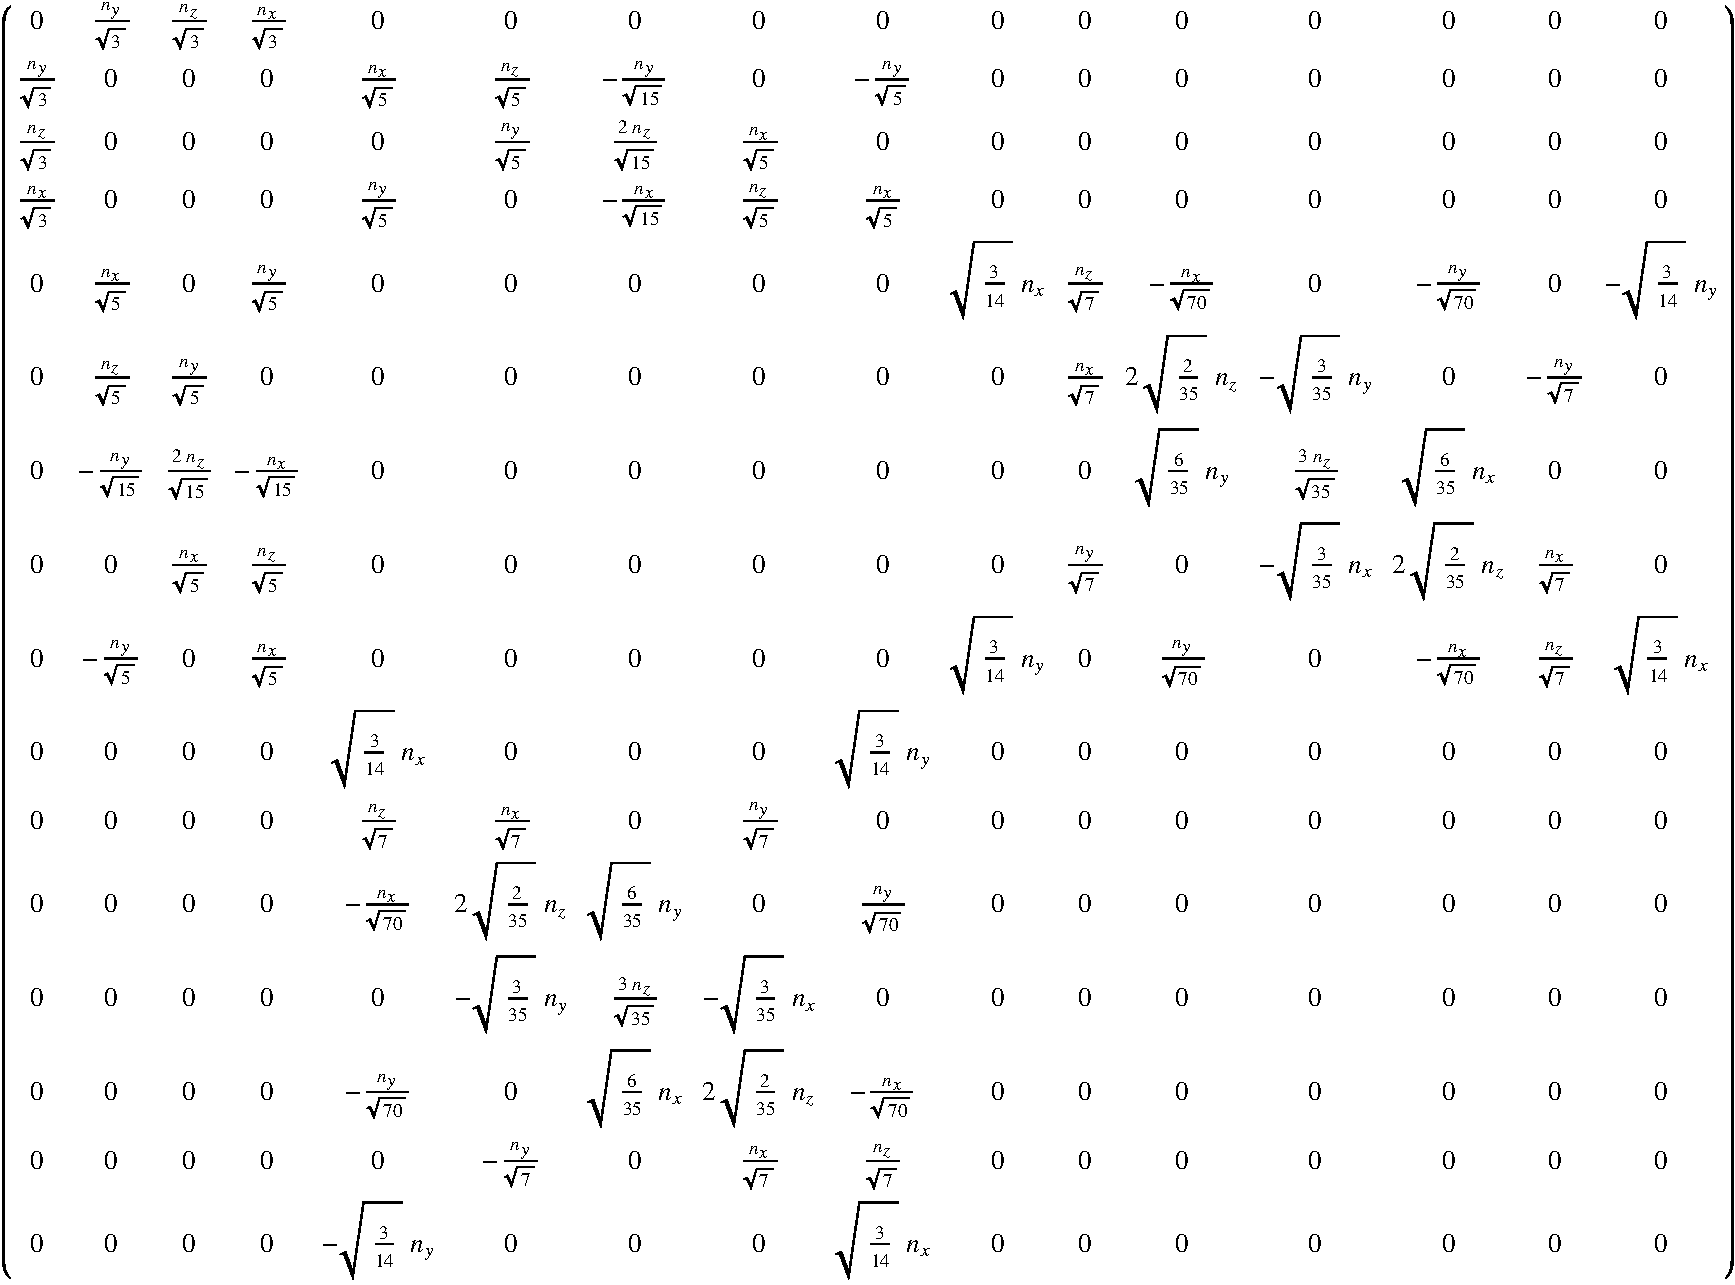
\includegraphics[scale=.575]{nA_P3}
  \caption{$\mat{A}_{\PN[3]}^{\bn}$}
  \label{fig:nAP3}
\end{figure}

Its eigendecomposition
shows that speed of propagation is uniform for all $\bn\in\R[3]$, given by the eigenvalues corresponding to the case
$\norm{\bn} = 1$ (written with their multiplicities):
$$
\begin{multlined}
\textstyle
\left\{0,0,0,0,-\sqrt{\frac{3}{7}},-\sqrt{\frac{3}{7}},\sqrt{\frac{3}{7}},\sqrt{\frac{3}{7}},-\frac{1}{\sqrt{7}},
-\frac{1}{\sqrt{7}},\frac{1}{\sqrt{7}},\frac{1}{\sqrt{7}},\right.\\
\textstyle
\left.-\sqrt{\frac{1}{35} \left(15-2 \sqrt{30}\right)},
\sqrt{\frac{1}{35} \left(15-2 \sqrt{30}\right)},-\sqrt{\frac{1}{35} \left(15+2 \sqrt{30}\right)},\sqrt{\frac{1}{35} 
\left(15+2 \sqrt{30}\right)}\right\}
\end{multlined} 
$$


\begin{remark}[\textsc{Time dependent problems}] 
Let us compare the nullspaces of $\PN[2]$ advection matrix $\mat{A}_{P_2}^{\bn}$: 
$$
\left[
\begin{array}{ccc}
 \frac{\sqrt{\frac{3}{5}} \left(n_z^2-1\right)}{1-2 n_y^2} & \frac{2 \sqrt{\frac{3}{5}} n_x n_z}{1-2 n_y^2} & \frac{\frac{3 n_z^2}{2 n_y^2-1}+1}{\sqrt{5}} \\
 0 & 0 & 0 \\
 0 & 0 & 0 \\
 0 & 0 & 0 \\
 \frac{n_x \left(n_z^2-2 n_y^2\right)}{n_y \left(2 n_y^2-1\right)} & -\frac{n_z-2 n_z^3}{n_y-2 n_y^3} & \frac{\sqrt{3} n_x n_z^2}{n_y-2 n_y^3} \\
 -\frac{n_z-n_z^3}{n_y-2 n_y^3} & \frac{n_x \left(-2 n_y^2-2 n_z^2+1\right)}{n_y \left(2 n_y^2-1\right)} & \frac{\sqrt{3} n_z \left(2 n_y^2+n_z^2-1\right)}{n_y \left(2 n_y^2-1\right)} \\
 0 & 0 & 1 \\
 0 & 1 & 0 \\
 1 & 0 & 0 \\
\end{array}
\right]
$$

\noindent and $\PN[3]$ advection matrix $\mat{A}_{P_3}^{\bn}$:

$$
\hspace*{-3.5cm}
\scriptsize
\left[
\begin{array}{cccc}
 0 & 0 & 0 & 0 \\
 \frac{\sqrt{\frac{15}{14}} n_x \left(n_z^2-1\right)}{n_y \left(4 n_y^2-3\right)} & \frac{\sqrt{\frac{5}{7}} n_z \left(2 n_y^2+3 n_z^2-3\right)}{n_y \left(4 n_y^2-3\right)} & \frac{n_x \left(-4 n_y^2-15 n_z^2+3\right)}{\sqrt{14} n_y \left(4 n_y^2-3\right)} & \frac{\sqrt{\frac{3}{7}} n_z \left(-4 n_y^2-5 n_z^2+3\right)}{n_y \left(4 n_y^2-3\right)} \\
 -\frac{\sqrt{\frac{30}{7}} n_x n_z \left(n_z^2-1\right)}{8 n_y^4-10 n_y^2+3} & -\frac{\sqrt{\frac{5}{7}} \left(2 n_z^2-1\right) \left(4 n_y^2+3 n_z^2-3\right)}{8 n_y^4-10 n_y^2+3} & \frac{5 \sqrt{\frac{2}{7}} n_x \left(n_y^2-3 n_x^2\right) n_z}{8 n_y^4-10 n_y^2+3} & \frac{\sqrt{\frac{3}{7}} \left(8 n_y^4-10 n_y^2+10 n_z^4+5 \left(4 n_y^2-3\right) n_z^2+3\right)}{8 n_y^4-10 n_y^2+3} \\
 -\frac{\sqrt{\frac{15}{14}} \left(2 n_y^2-2 n_z^2-1\right) \left(n_z^2-1\right)}{8 n_y^4-10 n_y^2+3} & \frac{2 \sqrt{\frac{5}{7}} n_x n_z \left(2 n_y^2-3 n_z^2\right)}{8 n_y^4-10 n_y^2+3} & \frac{8 n_y^4-10 \left(n_z^2+1\right) n_y^2-30 n_z^4+15 n_z^2+3}{\sqrt{14} \left(8 n_y^4-10 n_y^2+3\right)} & \frac{10 \sqrt{\frac{3}{7}} n_x n_z^3}{8 n_y^4-10 n_y^2+3} \\
 0 & 0 & 0 & 0 \\
 0 & 0 & 0 & 0 \\
 0 & 0 & 0 & 0 \\
 0 & 0 & 0 & 0 \\
 0 & 0 & 0 & 0 \\
 \frac{n_x \left(-8 n_y^4+\left(4 n_z^2+6\right) n_y^2-3 n_z^4+n_z^2-1\right)}{n_y \left(8 n_y^4-10 n_y^2+3\right)} & \frac{\sqrt{\frac{3}{2}} n_z \left(-6 n_z^4+5 n_z^2-1\right)}{n_y \left(8 n_y^4-10 n_y^2+3\right)} & \frac{\sqrt{15} n_x n_z^2 \left(3 n_z^2-1\right)}{n_y \left(8 n_y^4-10 n_y^2+3\right)} & \frac{\sqrt{\frac{5}{2}} n_z^3 \left(4 n_y^2+6 n_z^2-5\right)}{n_y \left(8 n_y^4-10 n_y^2+3\right)} \\
 \frac{\sqrt{\frac{3}{2}} n_z \left(-4 n_z^4+5 n_z^2-1\right)}{n_y \left(8 n_y^4-10 n_y^2+3\right)} & -\frac{n_x \left(2 n_y^2-3 n_z^2\right) \left(4 n_y^2+4 n_z^2-3\right)}{n_y \left(8 n_y^4-10 n_y^2+3\right)} & \frac{\sqrt{\frac{5}{2}} n_z \left(4 n_y^2+3 n_z^2-3\right) \left(4 n_z^2-1\right)}{n_y \left(8 n_y^4-10 n_y^2+3\right)} & \frac{\sqrt{15} n_x n_z^2 \left(-4 n_y^2-4 n_z^2+3\right)}{n_y \left(8 n_y^4-10 n_y^2+3\right)} \\
 \frac{\sqrt{15} n_x n_z^2 \left(n_z^2-1\right)}{n_y \left(8 n_y^4-10 n_y^2+3\right)} & \frac{\sqrt{\frac{5}{2}} n_z \left(2 n_z^2-1\right) \left(4 n_y^2+3 n_z^2-3\right)}{n_y \left(8 n_y^4-10 n_y^2+3\right)} & -\frac{n_x \left(8 n_y^4-10 n_y^2+15 n_z^4+5 \left(4 n_y^2-3\right) n_z^2+3\right)}{n_y \left(8 n_y^4-10 n_y^2+3\right)} & -\frac{\sqrt{\frac{3}{2}} n_z \left(16 n_y^4+20 \left(n_z^2-1\right) n_y^2+10 n_z^4-15 n_z^2+6\right)}{n_y \left(8 n_y^4-10 n_y^2+3\right)} \\
 0 & 0 & 0 & 1 \\
 0 & 0 & 1 & 0 \\
 0 & 1 & 0 & 0 \\
 1 & 0 & 0 & 0 \\
\end{array}
\right]
$$

\noindent Unlike the $\PN[3]$ approximation, we can see that the $\PN[2]$ approximation contains in its advection
nullspace nonzero components of the 0-th moment of angular flux, which is proportional to the scalar flux (total spatial neutron 
density). Therefore, as a consequence of $\PN[2]$ approximation, not all scalar flux components are propagated by the
action $\mat{A}_{P_2}^{\bn} \Psi$. It turns out that this is true for any even-order $\PN$ approximation, which is
``probably the most salient argument why even-order expansions should be shunned for time dependent problems'' 
\cite[p. 20]{McClarren5}.
\end{remark}
  
%: Declaration of originality
%\begin{declaration}

I hereby declare that this doctoral thesis is my own work, unless clearly stated otherwise.
\vspace{1cm}

\begin{flushright}
 \ldots\ldots\ldots\ldots\ldots\ldots\ldots\ldots\ldots\\
 Milan Hanu{\v s}~~~~~~~~~~
\end{flushright}
	
\end{declaration}
\printindex

\end{document}
